% CVPR 2025 Paper Template; see https://github.com/cvpr-org/author-kit

\documentclass[10pt,twocolumn,letterpaper]{article}

%%%%%%%%% PAPER TYPE  - PLEASE UPDATE FOR FINAL VERSION
\usepackage{cvpr}              % To produce the CAMERA-READY version
% \usepackage[review]{cvpr}      % To produce the REVIEW version
\usepackage{subcaption}
\usepackage{tikz}
\usepackage{makecell}
% \usepackage[pagenumbers]{cvpr} % To force page numbers, e.g. for an arXiv version

% Import additional packages in the preamble file, before hyperref
%
% --- inline annotations
%
\newcommand{\red}[1]{{\color{red}#1}}
\newcommand{\todo}[1]{{\color{red}#1}}
\newcommand{\TODO}[1]{\textbf{\color{red}[TODO: #1]}}
% --- disable by uncommenting  
% \renewcommand{\TODO}[1]{}
% \renewcommand{\todo}[1]{#1}



% It is strongly recommended to use hyperref, especially for the review version.
% hyperref with option pagebackref eases the reviewers' job.
% Please disable hyperref *only* if you encounter grave issues, 
% e.g. with the file validation for the camera-ready version.
%
% If you comment hyperref and then uncomment it, you should delete *.aux before re-running LaTeX.
% (Or just hit 'q' on the first LaTeX run, let it finish, and you should be clear).
\definecolor{cvprblue}{rgb}{0.21,0.49,0.74}
\usepackage[pagebackref,breaklinks,colorlinks,allcolors=cvprblue]{hyperref}

%%%%%%%%% PAPER ID  - PLEASE UPDATE
% \def\paperID{7} % *** Enter the Paper ID here
\def\confName{CVPR}
\def\confYear{2025}

%%%%%%%%% TITLE - PLEASE UPDATE
\title{LMFormer: Lane based Motion Prediction Transformer}

%%%%%%%%% AUTHORS - PLEASE UPDATE
\author{
    Harsh Yadav$^1$ \quad Maximilian Sch\"afer$^2$ \quad Kun Zhao$^2$ \quad Tobias Meisen$^1$\\
    $^1$University of Wuppertal, Germany \quad $^2$ Aptiv Services Deutschland GmbH \\
    {\tt\small {harsh.yadav@uni-wuppertal.de}}
}

\usepackage{acro}

\DeclareAcronym{ad}{
	short=AD,
	long=Autonomous Driving,
}

\DeclareAcronym{adas}{
	short=ADAS,
	long=Advance Driver Assistance Systems,
}
\DeclareAcronym{hd}{
	short=HD,
	long=High Definition,
}
\DeclareAcronym{gnn}{
	short=GNN,
	long=Graph Neural Network,
}
\DeclareAcronym{bev}{
	short=BEV,
	long=Bird-Eye-View,
}
\DeclareAcronym{msda}{
	short=MSDA,
	long=Multi-Scale-Deformable-Attention,
}
\DeclareAcronym{cnn}{
	short=CNN,
	long=Convolutional Neural Network,
}
\DeclareAcronym{GAN}{
	short=GAN,
	long=Generative Adversial Network,
}
\DeclareAcronym{VAE}{
	short=VAE,
	long=Variational Autoencoder,
}
\DeclareAcronym{detr}{
	short=DETR,
	long=Detection Transformer,
}
\DeclareAcronym{dino}{
	short=DINO,
	long=DETR with Improved deNoising anchOr box,
}
\DeclareAcronym{caspformer}{
	short=CASPFormer,
	long=Context Aware Scene Prediction Transformer,
}
\DeclareAcronym{caspnet}{
	short=CASPNet,
	long=Context Aware Scene Prediction Network,
}
\DeclareAcronym{mlp}{
	short=MLP,
	long=Multi-Layer Perceptron,
}
\DeclareAcronym{cv}{
	short=CV,
	long=Computer Vision,
}
\DeclareAcronym{wta}{
	short=WTA,
	long=Winner-Takes-All,
}
\DeclareAcronym{nll}{
	short=NLL,
	long=Negative Log Likelihood,
}


\begin{document}
\maketitle
\begin{abstract}
The ABSTRACT is to be in fully justified italicized text, at the top of the left-hand column, below the author and affiliation information.
Use the word ``Abstract'' as the title, in 12-point Times, boldface type, centered relative to the column, initially capitalized.
The abstract is to be in 10-point, single-spaced type.
Leave two blank lines after the Abstract, then begin the main text.
Look at previous \confName abstracts to get a feel for style and length.
\end{abstract}    
\section{Introduction}
\label{sec:intro}

Please follow the steps outlined below when submitting your manuscript to the IEEE Computer Society Press.
This style guide now has several important modifications (for example, you are no longer warned against the use of sticky tape to attach your artwork to the paper), so all authors should read this new version.

%-------------------------------------------------------------------------
\subsection{Language}

All manuscripts must be in English.

\subsection{Dual submission}

Please refer to the author guidelines on the \confName\ \confYear\ web page for a
discussion of the policy on dual submissions.

\subsection{Paper length}
Papers, excluding the references section, must be no longer than eight pages in length.
The references section will not be included in the page count, and there is no limit on the length of the references section.
For example, a paper of eight pages with two pages of references would have a total length of 10 pages.
{\bf There will be no extra page charges for \confName\ \confYear.}

Overlength papers will simply not be reviewed.
This includes papers where the margins and formatting are deemed to have been significantly altered from those laid down by this style guide.
Note that this \LaTeX\ guide already sets figure captions and references in a smaller font.
The reason such papers will not be reviewed is that there is no provision for supervised revisions of manuscripts.
The reviewing process cannot determine the suitability of the paper for presentation in eight pages if it is reviewed in eleven.

%-------------------------------------------------------------------------
\subsection{The ruler}
The \LaTeX\ style defines a printed ruler which should be present in the version submitted for review.
The ruler is provided in order that reviewers may comment on particular lines in the paper without circumlocution.
If you are preparing a document using a non-\LaTeX\ document preparation system, please arrange for an equivalent ruler to appear on the final output pages.
The presence or absence of the ruler should not change the appearance of any other content on the page.
The camera-ready copy should not contain a ruler.
(\LaTeX\ users may use options of \texttt{cvpr.sty} to switch between different versions.)

Reviewers:
note that the ruler measurements do not align well with lines in the paper --- this turns out to be very difficult to do well when the paper contains many figures and equations, and, when done, looks ugly.
Just use fractional references (\eg, this line is $087.5$), although in most cases one would expect that the approximate location will be adequate.


\subsection{Paper ID}
Make sure that the Paper ID from the submission system is visible in the version submitted for review (replacing the ``*****'' you see in this document).
If you are using the \LaTeX\ template, \textbf{make sure to update paper ID in the appropriate place in the tex file}.


\subsection{Mathematics}

Please number all of your sections and displayed equations as in these examples:
\begin{equation}
  E = m\cdot c^2
  \label{eq:important}
\end{equation}
and
\begin{equation}
  v = a\cdot t.
  \label{eq:also-important}
\end{equation}
It is important for readers to be able to refer to any particular equation.
Just because you did not refer to it in the text does not mean some future reader might not need to refer to it.
It is cumbersome to have to use circumlocutions like ``the equation second from the top of page 3 column 1''.
(Note that the ruler will not be present in the final copy, so is not an alternative to equation numbers).
All authors will benefit from reading Mermin's description of how to write mathematics:
\url{http://www.pamitc.org/documents/mermin.pdf}.

\subsection{Blind review}

Many authors misunderstand the concept of anonymizing for blind review.
Blind review does not mean that one must remove citations to one's own work---in fact it is often impossible to review a paper unless the previous citations are known and available.

Blind review means that you do not use the words ``my'' or ``our'' when citing previous work.
That is all.
(But see below for tech reports.)

Saying ``this builds on the work of Lucy Smith [1]'' does not say that you are Lucy Smith;
it says that you are building on her work.
If you are Smith and Jones, do not say ``as we show in [7]'', say ``as Smith and Jones show in [7]'' and at the end of the paper, include reference 7 as you would any other cited work.

An example of a bad paper just asking to be rejected:
\begin{quote}
\begin{center}
    An analysis of the frobnicatable foo filter.
\end{center}

   In this paper we present a performance analysis of our previous paper [1], and show it to be inferior to all previously known methods.
   Why the previous paper was accepted without this analysis is beyond me.

   [1] Removed for blind review
\end{quote}


An example of an acceptable paper:
\begin{quote}
\begin{center}
     An analysis of the frobnicatable foo filter.
\end{center}

   In this paper we present a performance analysis of the  paper of Smith \etal [1], and show it to be inferior to all previously known methods.
   Why the previous paper was accepted without this analysis is beyond me.

   [1] Smith, L and Jones, C. ``The frobnicatable foo filter, a fundamental contribution to human knowledge''. Nature 381(12), 1-213.
\end{quote}

If you are making a submission to another conference at the same time, which covers similar or overlapping material, you may need to refer to that submission in order to explain the differences, just as you would if you had previously published related work.
In such cases, include the anonymized parallel submission~\cite{Authors14} as supplemental material and cite it as
\begin{quote}
[1] Authors. ``The frobnicatable foo filter'', F\&G 2014 Submission ID 324, Supplied as supplemental material {\tt fg324.pdf}.
\end{quote}

Finally, you may feel you need to tell the reader that more details can be found elsewhere, and refer them to a technical report.
For conference submissions, the paper must stand on its own, and not {\em require} the reviewer to go to a tech report for further details.
Thus, you may say in the body of the paper ``further details may be found in~\cite{Authors14b}''.
Then submit the tech report as supplemental material.
Again, you may not assume the reviewers will read this material.

Sometimes your paper is about a problem which you tested using a tool that is widely known to be restricted to a single institution.
For example, let's say it's 1969, you have solved a key problem on the Apollo lander, and you believe that the 1970 audience would like to hear about your
solution.
The work is a development of your celebrated 1968 paper entitled ``Zero-g frobnication: How being the only people in the world with access to the Apollo lander source code makes us a wow at parties'', by Zeus \etal.

You can handle this paper like any other.
Do not write ``We show how to improve our previous work [Anonymous, 1968].
This time we tested the algorithm on a lunar lander [name of lander removed for blind review]''.
That would be silly, and would immediately identify the authors.
Instead write the following:
\begin{quotation}
\noindent
   We describe a system for zero-g frobnication.
   This system is new because it handles the following cases:
   A, B.  Previous systems [Zeus et al. 1968] did not  handle case B properly.
   Ours handles it by including a foo term in the bar integral.

   ...

   The proposed system was integrated with the Apollo lunar lander, and went all the way to the moon, don't you know.
   It displayed the following behaviours, which show how well we solved cases A and B: ...
\end{quotation}
As you can see, the above text follows standard scientific convention, reads better than the first version, and does not explicitly name you as the authors.
A reviewer might think it likely that the new paper was written by Zeus \etal, but cannot make any decision based on that guess.
He or she would have to be sure that no other authors could have been contracted to solve problem B.
\medskip

\noindent
FAQ\medskip\\
{\bf Q:} Are acknowledgements OK?\\
{\bf A:} No.  Leave them for the final copy.\medskip\\
{\bf Q:} How do I cite my results reported in open challenges?
{\bf A:} To conform with the double-blind review policy, you can report results of other challenge participants together with your results in your paper.
For your results, however, you should not identify yourself and should not mention your participation in the challenge.
Instead present your results referring to the method proposed in your paper and draw conclusions based on the experimental comparison to other results.\medskip\\

\begin{figure}[t]
  \centering
  \fbox{\rule{0pt}{2in} \rule{0.9\linewidth}{0pt}}
   %\includegraphics[width=0.8\linewidth]{egfigure.eps}

   \caption{Example of caption.
   It is set in Roman so that mathematics (always set in Roman: $B \sin A = A \sin B$) may be included without an ugly clash.}
   \label{fig:onecol}
\end{figure}

\subsection{Miscellaneous}

\noindent
Compare the following:\\
\begin{tabular}{ll}
 \verb'$conf_a$' &  $conf_a$ \\
 \verb'$\mathit{conf}_a$' & $\mathit{conf}_a$
\end{tabular}\\
See The \TeX book, p165.

The space after \eg, meaning ``for example'', should not be a sentence-ending space.
    So \eg is correct, {\em e.g.} is not.
The provided \verb'\eg' macro takes care of this.

When citing a multi-author paper, you may save space by using ``et alia'', shortened to ``\etal'' (not ``{\em et.\ al.}'' as ``{\em et}'' is a complete word).
If you use the \verb'\etal' macro provided, then you need not worry about double periods when used at the end of a sentence as in Alpher \etal.
However, use it only when there are three or more authors.
Thus, the following is correct:
   ``Frobnication has been trendy lately.
   It was introduced by Alpher~\cite{Alpher02}, and subsequently developed by
   Alpher and Fotheringham-Smythe~\cite{Alpher03}, and Alpher \etal~\cite{Alpher04}.''

This is incorrect: ``... subsequently developed by Alpher \etal~\cite{Alpher03} ...'' because reference~\cite{Alpher03} has just two authors.

\begin{figure*}
  \centering
  \begin{subfigure}{0.68\linewidth}
    \fbox{\rule{0pt}{2in} \rule{.9\linewidth}{0pt}}
    \caption{An example of a subfigure.}
    \label{fig:short-a}
  \end{subfigure}
  \hfill
  \begin{subfigure}{0.28\linewidth}
    \fbox{\rule{0pt}{2in} \rule{.9\linewidth}{0pt}}
    \caption{Another example of a subfigure.}
    \label{fig:short-b}
  \end{subfigure}
  \caption{Example of a short caption, which should be centered.}
  \label{fig:short}
\end{figure*}

\section{Related Work}\label{section:related_work}
The lane-aware trajectory prediction task primarily involves three important challenges: scene representation, learning a lane graph, and forcing the diversity in the outputs. We review some of the important related work for these strategies in this section.

\subsection{Scene Representation}\label{subsection:scene_rep}
Earlier works \cite{cui2019multimodal,chai2019multipath} rely on rasterized representations of the surrounding scene, where static and dynamic context information is stored across the channel dimension. These representations allow for the use of \acp{cnn} to extract meaningful features. However, rasterized representations suffer from limited resolution and include redundant pixel information, motivating the exploration of more compact scene representations. LaneGCN \cite{liang2020learning} first introduced the idea that HD maps inherently possess a graph structure, leveraging graph convolution to encode this information. Building on this, VectorNet \cite{gao2020vectornet} proposed a unified vector representation for various scene elements, including lanes, crosswalks, traffic lights, and surrounding agents. Despite these innovations, vector-based approaches face a limitation: they encode scene elements from the perspective of the target vehicle, necessitating re-normalization and re-encoding at each time step, which introduces redundant computations. QCNet \cite{zhou2023query} addresses this issue by adopting a query-centric approach. It encodes each scene element in its own coordinate frame, removing the need for re-normalization and re-encoding. Additionally, QCNet employs temporal and spatial embeddings to capture relative information across scene elements effectively. In our work, we adopt the query-centric vector-based approach to encode scene elements, as it offers lower computational complexity compared to agent-centric and rasterized representations.

\subsection{Lane Graph} \label{subsection:lane_graph}
The lane information in the static context for motion prediction tasks is typically stored as lane polylines. Each polyline is represented as $L_p^i = [P_1^i, P_2^i, ...., P_K^i]$, where $K$ denotes the number of control points in the polyline $i$, and $P_k^i$ denotes the position of these control points in the global coordinate system. Prior studies \cite{gao2020vectornet,ngiam2021scene,liu2024laformer} first transform the polylines into the target agent coordinate system before generating their corresponding encodings. On the other hand, the approaches \cite{liang2020learning,wang2022ltp,zhou2022hivt,zhou2023query} first convert the point-based representation of the polylines to segment-based representation; $L_v^i = [V_1^i, V_2^i, ...., V_{K-1}^i]$, where $V_{k}^i = [P_k^i, P_{k+1}^i]$ stores the vector information of lane segments. In this case, the lane features are generated from the vectors of individual segments. The advantage of the segment-based approach is that road curvature is explicitly encoded in the lane encodings. A potential limitation of all the aforementioned approaches is that they fail to use explicit information on lane connections at intersections, lane splits, and lane merges. 
Sun et al. \cite{sun2024semanticformer} attempt to use lane connection information to generate consistent lanes. However, their method requires an extensive map ontology, the creation and maintenance of which is expensive and thus has limited scalability. Therefore, in our work, we propose a simple mechanism to use the lane connection information together with the segment-based representation. This integrated approach not only achieves SOTA performance, but also improves the explainability of the prediction module.  

% LaneGCN \cite{liang2020learning} pioneered the idea that lanes are among the most important static context elements for motion prediction modules. However, its convolution-based architecture performs poorly in comparison to other transformer-based approaches \cite{ngiam2021scene,zhou2022hivt}. Wang et al. \cite{wang2022ltp} argue that lane segments within the static context are particularly suitable for behavioral intent modeling. However, the authors model this intent independently of the prediction task, using a three-layer MLP to score individual lane segments. Similarly, Liu et al. \cite{liu2024laformer} score the top-k potential lane segments through interaction graphs and subsequently decode trajectories using contextual information gathered from these selected segments. In parallel, Sun et al. \cite{sun2024semanticformer} propose generating Meta-Paths based solely on static context, representing paths that the target vehicle could traverse in the near future. These learned Meta-Paths are then utilized as anchors for predicting future trajectories. A common limitation of these aforementioned approaches is that the attention mechanisms used for extracting contextual information from road lanes operate independently of the prediction task. In contrast, our work incorporates lane awareness directly into the Transformer attention mechanism within the motion prediction module. This integrated approach not only achieves SOTA performance but also enhances the explainability of the prediction module.  

\subsection{Multi-Modal Prediction}\label{section:multi-modal-prediction}
To safely plan paths in complex traffic scenarios, motion prediction modules must generate multiple modes, each representing a scene-consistent trajectory. The advent of vector-based scene representations has enabled researchers to explore techniques such as \acp{VAE} \cite{casas2020implicit,cui2021lookout} and \acp{GAN} \cite{huang2020diversitygan} for producing diverse trajectory predictions. However, these approaches often suffer from mode collapse, where all predicted modes converge to a single trajectory with minor variations. In contrast, transformer architectures leveraging learnable anchors have achieved notable success in generating diverse trajectory predictions \cite{liu2021multimodal,ngiam2021scene,zhou2022hivt,zhou2023query}. Current SOTA methods build on transformer backbones and incorporate advanced techniques, including asked auto encoders \cite{cheng2023forecast,lan2023sept}, knowledge graphs \cite{sun2024semanticformer}, and language models \cite{seff2023motionlm}. These approaches have been extensively validated on open-source datasets such as nuScenes \cite{caesar2020nuscenes}, Argoverse \cite{chang2019argoverse}, Argoverse 2 \cite{wilson2023argoverse}, and Waymo \cite{mei2022waymo}. Building on this trend, UniTraj \cite{feng2024unitraj} introduces a unified framework that consolidates different datasets, network architectures, and evaluation criteria, enabling the development of larger and more generalized models.
\section{Approach}\label{section:approach}
In this section, we describe the input-output formulation and the network architecture. We further provide a mathematical illustration of the loss function. 
\begin{figure}
    \centering
    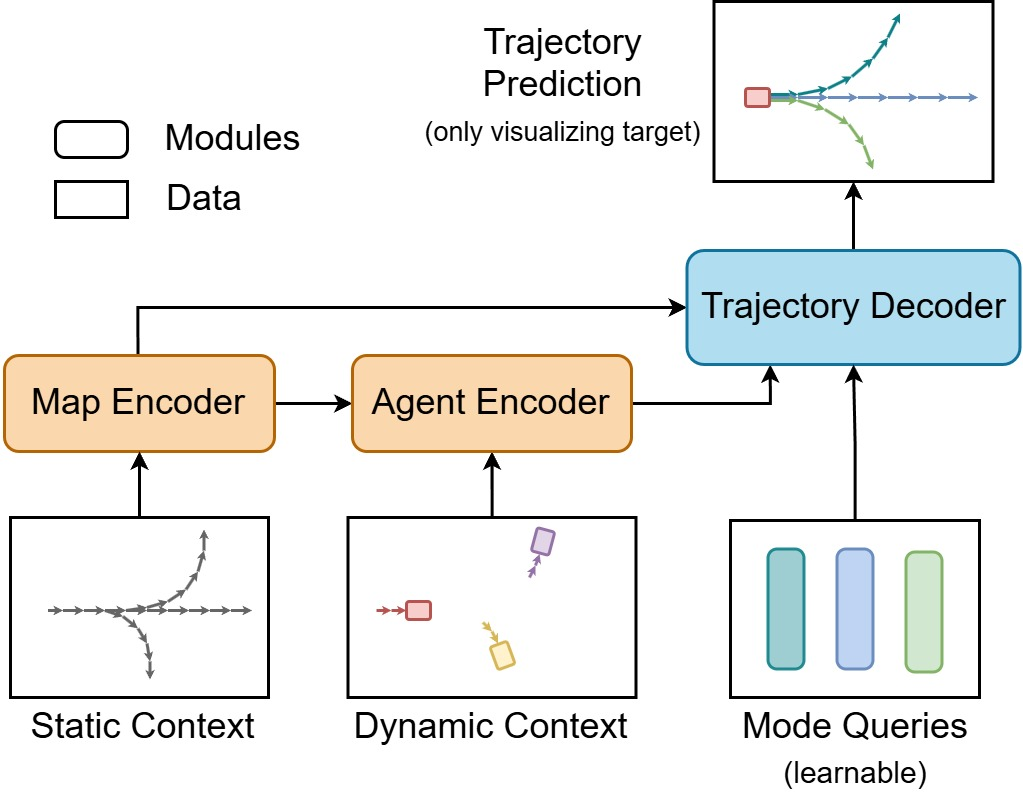
\includegraphics[width=0.9\linewidth]{images/lane_based_prediction_overall_architecture.jpg}
    \caption{An Illustration of LMFormer architecture. We employ a transformer-based encoder-decoder architecture to generate multiple scene-consistent trajectories for all the dynamic agents. Notably the static context only consists of lane segments.}
    \label{fig:overall_net}
\end{figure}

\subsection{Input-Output Formulation}\label{subsection:IO_formulation}
The input to LMFormer consists of the positions of surrounding lanes and dynamic agents in the scene. As described in section \ref{subsection:scene_rep}, we opt for a query-centric representation \cite{zhou2023query} of each scene element. This representation eliminates the need for redundant agent-centric encodings at each time step, thereby reducing the computational overhead associated with repeated coordinate transformations as well as encoding generation. Below, we detail how we compute the query-centric coordinates and features for both static and dynamic contexts. In addition, we also illustrate the formulation of the output trajectory in vector format.

\noindent\textbf{Static Context:} As described in section \ref{subsection:lane_graph}, the static context consists of lane polylines from which lane segments are generated. Every lane segment is characterized by its start and end positions in global coordinates. The query-centric coordinate frame for a lane segment is set as follows: we designate the segment’s start position as its origin and align the segment's vector direction with its x-axis. As a result, the only feature preserved in this query-centric coordinate frame is the segment's length, which we use as its sole feature in the query-centric embedding generation.

\begin{figure}
    \centering
    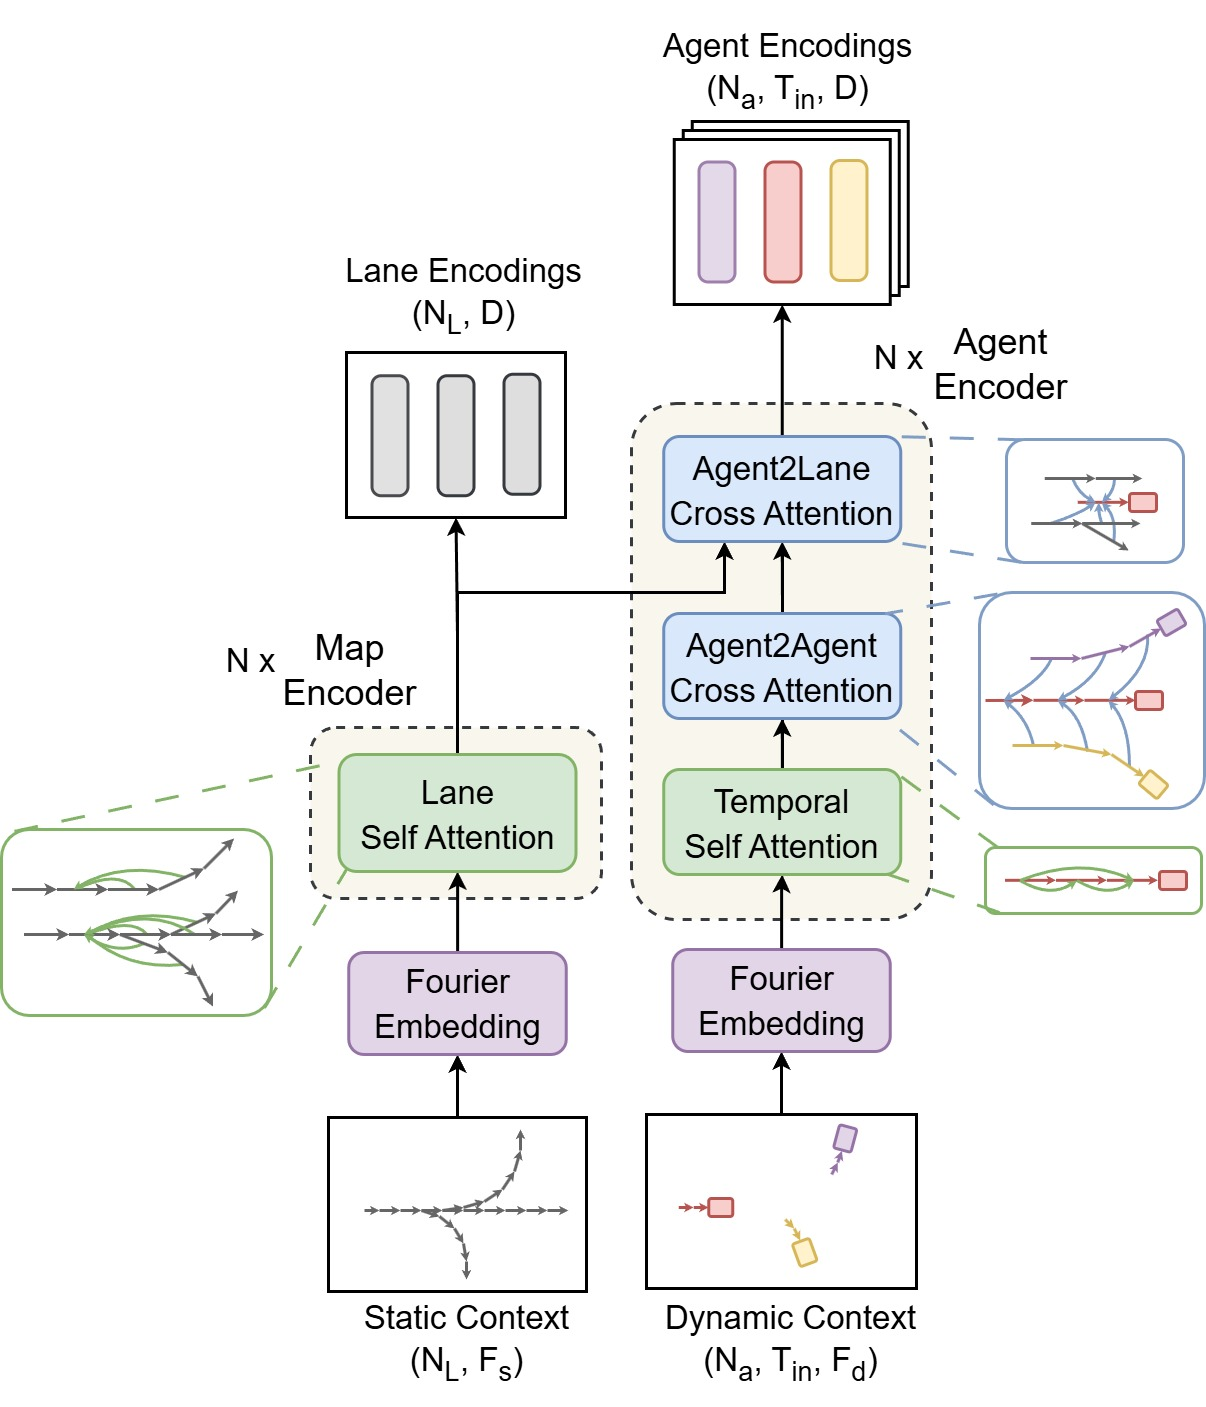
\includegraphics[width=1\linewidth]{images/lane_based_prediction_encoder_paper.jpg}
    \caption{The encoder receives Static and Dynamic context as input and it outputs Lanes and Agents Encodings. The encoder is divided into two parts: Map Encoder and Agent Encoder. The Map Encoder models the long-range interaction among the lane segments. The Agent Encoder models the interaction of all the surrounding static and dynamic elements into each agent's latent embedding. The attention mechanisms are illustrated by green (self-attention) and blue (cross-attention) arrows, where the arrowheads point toward the queries and the tails point away from keys/values. The encoders repeat the interaction modeling N times, to learn complex interactions, where the weights across each layer are not shared.}
    \label{fig:encoder}
\end{figure}

\noindent\textbf{Dynamic Context:} For the dynamic context, agent trajectories are provided as $\mathcal{T}_{in}^a = [P_1^a, P_2^a, ..., P_T^a]$ with global positions $P_t^a$. Motion vectors $M_t^a = [P_t^a, P_{t+1}^a]$ are derived at each time step from these trajectories, encapsulating the agent’s start and end positions within that interval. The query-centric coordinate frame for a motion vector is determined as follows: we set the motion vector’s start position as its origin and align the agent’s instantaneous direction of travel with its x-axis. Notably, the motion vector’s direction may differ from the instantaneous direction of travel, introducing an angular deviation from the x-axis. Consequently, in the query-centric representation, we encode the motion vector’s length and its orientation relative to the x-axis as its features. 

\noindent\textbf{Output Representation:} The output can be represented as  $\mathcal{T}_{out}^{a,m} = [(V_1^{a,m}, S_1^{a,m}), (V_2^{a,m}, S_2^{a,m}), ..., (V_{T'}^{a,m}, S_{T'}^{a,m})]$, where $T'$ is the temporal length of the future trajectories, and $V_t^{a,m} = [P_{t-1}^{a,m}, P_t^{a,m}]$ is the motion vector corresponding to agent $a$, mode $m$, and time step $t$, with an associated variance of $S_t^{a,m}$. The query-centric coordinate frame for these motion vectors is defined as the last observed position and the current direction of travel of the corresponding agent. The predicted future trajectories are reconstructed from these motion vectors in the global coordinate frame, preserving mean positions and associated variances at each time step. Additionally, we predict the probability distribution over predicted trajectories, quantifying the likelihood of each mode.

\subsection{Network Architecture}\label{subsection:network_architecture}
Our model follows a transformer-based encoder-decoder architecture, where the decoder generates scene-consistent trajectories from the latent scene encodings produced by the encoder, as shown in Figure \ref{fig:overall_net}.

\subsubsection{Encoder}\label{subsubsection:encoder}
The encoder is designed to capture interactions between different scene elements. Our design leverages the fact that while the static context is independent of the dynamic context, the reverse does not hold. Consequently, we first encode the static context independently before incorporating it into the dynamic context encoding process. This necessitates two distinct encoders: a Map Encoder and an Agent Encoder, as illustrated in Figure \ref{fig:encoder}. Given the high-frequency nature of motion vectors, we apply learnable Fourier Embeddings \cite{tancik2020fourier} to all scene elements prior to modeling interactions within the encoder.

The Map Encoder is responsible for capturing long-range interactions between lane segments. To construct this interaction graph, we exploit the fact that the most relevant contextual information for each lane segment is present in the lane segments accessible via traversing in the direction of travel. These interactions are modeled using multi-headed attention \cite{vaswani2017attention}, where each lane segment is represented by its query-centric feature embeddings. To capture the relative positions in the multi-headed attention, the keys/values are concatenated with relative position embeddings \cite{zhou2023query}. The Lane Self-Attention module is applied iteratively $N$ times, refining the lane encodings before passing them to the Agent Encoder and subsequent network components.

The Agent Encoder learns interactions between agents and their surrounding scene elements. It comprises three specialized attention modules:
\begin{itemize}
    \item Temporal Self-Attention: Captures dependencies across different time steps for the same agent.
    \item Agent2Agent Cross-Attention: Models interactions between different agents at a given time step.
    \item Agent2Lane Cross-Attention: Encodes contextual interactions from lane segments (keys/values) to agents (queries).
\end{itemize}
Similar to the Map Encoder, multi-headed attention with relative position embeddings is employed in the Agent Encoder. Each interaction module is applied iteratively $N$ times, producing Agent Encodings that serve as input for the trajectory decoder.

\subsubsection{Decoder}\label{subsubsection:decoder}

\begin{figure}
    \centering
    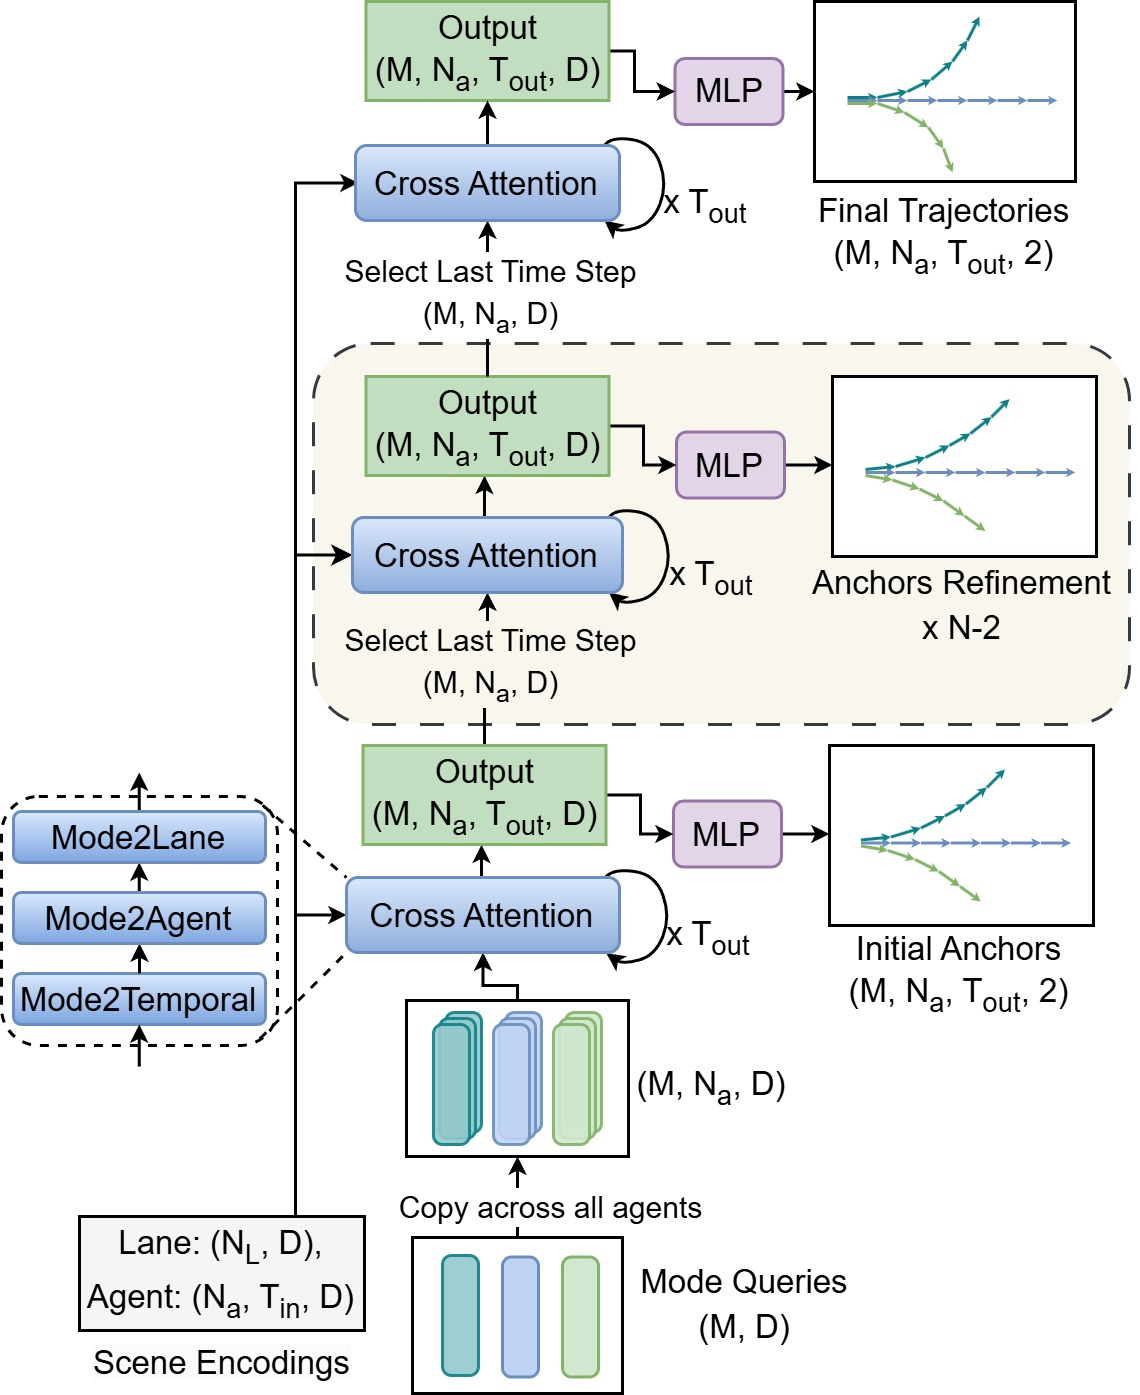
\includegraphics[width=1.\linewidth]{images/lane_based_prediction_decoder_paper.jpg}
    \caption{A depiction of the decoder architecture. The decoder performs cross-attention in between learnable mode queries and Scene Encodings (keys/values). The cross-attention layer is stacked N times and the intermittent output as well as the final output queries are transformed into trajectories with MLP. Thus we obtain N trajectories corresponding to each mode of every agent. During the training, all these N trajectories are trained against the ground truth, while during inference only the final layer output is generated. Importantly, the weights across the stacked cross-attention layers are not shared, while those in the MLP layers are.}
    \label{fig:decoder}
\end{figure}

To facilitate multimodal trajectory prediction, we introduce learnable mode queries, with each query corresponding to a distinct trajectory for every agent in the scene. Figure \ref{fig:decoder} shows the architecture of the decoder.

During initial experiments, we observed that the predicted trajectories exhibited jerky motion and, in some cases, misalignment with lane structures. To mitigate these issues, we drew inspiration from the iterative refinement of bounding boxes in DAB-DETR \cite{liu2022dabdetr}, where bounding boxes are progressively refined through offset computations after each transformer output layer. However, direct adaptation of this approach is impractical for trajectory prediction, as bounding boxes in computer vision are randomly initialized, whereas trajectory prediction requires a reliable set of initial predictions. Thus, instead of applying offset-based refinement at each transformer layer, we compute entire trajectories and compare them against the ground truth to derive additional refinement losses. Another important distinction from DAB-DETR is that LMFormer does not share the weights across each refinement layer, but rather uses the intermittent output from the multiple stacked layers. We show the effectiveness of the additional refinement loss in an ablation study.

Previous research \cite{yadav2025caspformer,zhou2023query} demonstrates that recurrent temporal decoding enhances trajectory prediction quality. Therefore, we incorporate recurrent decoding ($\times T_{out}$) in cross-attention modules. Each recurrent loop updates the query position as well as the query itself, similar to CASPFormer \cite{yadav2025caspformer}. The cross-attention module consists of three key attention mechanisms:
\begin{itemize}
    \item Mode2Temporal Cross Attention: Aggregates temporal information from Agent Encodings (keys/values) to modes (queries).
    \item Mode2Agent Cross Attention: Each mode of an agent attends to the same mode of the other agent in the scene.
    \item Mode2Lane Cross Attention: Enables mode queries to incorporate static context information from Lane Encodings (keys/values).
\end{itemize}

\subsection{Loss Formulation}\label{subsection:loss}
We model the predicted trajectories using a mixture model, which is trained to maximize the likelihood of the ground truth trajectory. The optimization objective is thus formulated as follows:

\begin{equation}
    \mathcal{L}(Y) = \sum_{m=1}^M \pi_m \prod_{t=1}^T P(Y^t | \mu_m^t, b_m^t),
    \label{eq:liklihood_function}
\end{equation}
where $Y$ represents the ground truth trajectory, $\pi_m$ denotes the probability of mode $m$, and $P(\cdot|\cdot)$ follows a Laplace distribution parameterized by the mean $\mu_m$ and scale $b_m$, which defines the positional uncertainty of the predicted trajectories. %In our initial experiments, we also tested Gaussian probability density functions as a candidate for $P(\cdot|\cdot)$, and identified that the network predicts more diverse predictions with the Laplace probability density function.

As shown by Rupprecht et al. \cite{rupprecht2017learning}, directly optimizing the \ac{nll} of mixture models can lead to numerical instability and mode collapse. To mitigate this, the mixture model optimization is decomposed into two objectives via separate regression and classification losses \cite{cui2019multimodal,makansi2019overcoming,zhou2022hivt,yadav2025caspformer}. In our approach, we adopt the \ac{wta} strategy, where the regression loss optimizes only the parameters of the best-matching mode and is defined as:

\begin{align}
    \mathrm{L}_{reg} & = - log \prod_{t=1}^T P(Y^t | \mu_{m*}^t, b_{m*}^t) \nonumber \\
                    & = - \sum_{t=1}^T log \ P(Y^t | \mu_{m*}^t, b_{m*}^t),
\end{align}
where $m^*$ is the mode with the smallest $L_2$ distance to the ground truth trajectory. For the classification loss, we optimize the \ac{nll} of the likelihood function shown in equation \eqref{eq:liklihood_function} as follows:

\begin{equation}
    \mathrm{L}_{cls} = - log \ \mathcal{L}(Y)
\end{equation}

To enhance training stability, we decouple the optimization: the classification loss updates only the mode probabilities $\pi_m$, while the regression loss optimizes the trajectory parameters $\mu_m$ and $b_m$. Finally, the total training loss is defined as the sum of classification and regression losses:

\begin{equation}
    \mathrm{L} = \lambda \ \mathrm{L}_{cls} + \sum_{n=2}^{N}\mathrm{L}_{reg},
\end{equation}
where $N$ denotes the number of stacked layers, and $\lambda$ controls the trade-off between classification and regression losses.
\section{Experiments}\label{section:experiments}
In this section, we present the experimental evaluation of LMFormer. We first describe the datasets and experimental setup, followed by a detailed quantitative and qualitative performance analysis. Our goal is to demonstrate the effectiveness of LMFormer on both standard benchmarks and real-world-inspired scenarios while also highlighting its generalization ability across different datasets.

\subsection{Experimental Setup}\label{subsection:exp_setup}
\textbf{Dataset:} As we aim to evaluate LMFormer’s performance in structured urban environments as well as more diverse intersection-heavy scenarios, we selected the nuScenes \cite{caesar2020nuscenes} and the Deep Scenario \cite{lu2023deepscenario} datasets for benchmarking. The nuScenes dataset comprises driving scenarios from Boston and Singapore, generated using sensor data of a moving vehicle in complex scenarios. The Deep Scenario dataset is built from recordings of stationary drones, placed vertically above complex traffic scenarios, e.g. intersections.

\noindent\textbf{Metrics:} We report the quantitative performance of LMFormer on the nuScenes and Deep Scenario datasets in terms of minADE\textsubscript{k}, minFDE\textsubscript{k}, MR\textsubscript{k}, and OffRoadRate. minADE\textsubscript{k} measures the average Euclidean distance between the ground truth and the best-matching trajectory among the top-$k$ predicted trajectories. A lower value indicates better alignment with the actual observed path. This metric is particularly relevant for multi-modal prediction settings, where multiple future outcomes are possible. minFDE\textsubscript{k} computes Euclidean distances between the endpoint of the ground truth and the best prediction among the top-$k$ trajectories. It indicates how well the network predicts the final goal position. MR\textsubscript{k} measures the fraction of misses, where a miss occurs when the maximum pointwise $L_2$ distance between the ground truth and predicted trajectories is larger than two meters. A small value indicates that the predicted velocity profile matches the ground truth well. Finally, the OffRoadRate metric reports the fraction of predicted trajectories outside the drivable area.

\noindent\textbf{Implementation Details:} We train LMFormer on one Nvidia A100 GPU using AdamW Optimizer \cite{loshchilov2018decoupled}. As required by nuScenes Prediction Challenge \cite{nuscene2020prediction}, the duration of the input trajectory is limited to 2 seconds and that of the output trajectory to 6 seconds, with a sampling rate of 2Hz.  Also, the maximum number of modes $k$ is set to 5, to compute minADE\textsubscript{5} and MR\textsubscript{5} for the comparison against other SOTA methods. The same configurations are extended to the Deep Scenario Dataset, as it does not specify any restrictions on the aforementioned hyperparameters. 

Both static and dynamic contexts enclose an area of 150m x 100m, where the former is along the driving direction. In order to help the model generalize for both left-hand and right-hand driving conditions, the inputs are flipped along the driving direction with a probability of 50\%. We also identify that increasing the number of stacked layers $N$ beyond 3 does not improve the network performance, and hence we set $N$ = 3 to keep the computational costs to a minimum. A similar observation is made for the length of a lane segment, and its optimum value is recorded at 3 meters. 

\subsection{Results and Discussion}\label{subsection:results}
\begin{table}[b]
    \centering
    \caption{Comparison with state-of-the-art on the nuScenes prediction challenge test split.}
    \label{tab:experiment_table}
    \resizebox{\linewidth}{!}{
    \begin{tabular}{l|c c|c|c}
    \hline
    Method & minADE\textsubscript{5}$\downarrow$ & MR\textsubscript{5}$\downarrow$ & minFDE\textsubscript{1}$\downarrow$ & OffRoad$\downarrow$ \\
    \hline
    GOHOME \cite{gilles2022gohome}  & 1.42 & 0.57 & 6.99 & 0.04 \\
    Autobot \cite{girgis2021latent}  & 1.37 & 0.62 & 8.19 & 0.02 \\
    THOMAS \cite{gilles2022thomas}  & 1.33 & 0.55 & 6.71 & 0.03 \\
    PGP \cite{deo2021multimodal}  & 1.27 & 0.52 & 7.17 & 0.03 \\
    MacFormer \cite{feng2023macformer}  & 1.21 & 0.57 & 7.50 & 0.02 \\
    LAFormer \cite{liu2024laformer}  & 1.19 & 0.48 & 6.95 & 0.02 \\
    Socialea \cite{chen2023q} & 1.18 & 0.48 & 6.77 & 0.03 \\
    FRM \cite{park2023leveraging}  & 1.18 & 0.48 & 6.59 & 0.02 \\
    CASPNet\_v2 \cite{schafer2023caspnet++} & 1.16 & 0.50  & \textbf{6.18} & \textbf{0.01} \\
    CASPFormer \cite{yadav2025caspformer} & 1.15 & 0.48 & 6.70 & \textbf{0.01} \\
    SemanticFormerR \cite{sun2024semanticformer} & \textbf{1.14} & 0.50 & 6.27 & 0.03 \\
    \hline
    LMFormer (ours) & \textbf{1.14} & \textbf{0.47} & 6.85 & \textbf{0.01} \\
    \hline
    \end{tabular}
    }
\end{table}

We provide a comparison of LMFormer against the SOTA networks on the nuScenes Motion Prediction Challenge test split \cite{nuscene2020prediction} in Table \ref{tab:experiment_table}. LMFormer achieves SOTA results across minADE\textsubscript{5}, MR\textsubscript{5} and OffRoadRate. Qualitative results are depicted in Figure \ref{fig:nuScenes_qual}. As is evident, the trajectories undergo a substantial enhancement during the refinement process. It is noteworthy that the network is capable of making diverse predictions and aligning the predicted trajectories with a high degree of accuracy with the lanes. Furthermore, the attention map provides insight into the underlying learning behaviors of LMFormer. We observe that the network pays higher attention to the lanes, which are important for predicting its future trajectory.

It is important to note that despite achieving SOTA performance across all other metrics, LMFormer does not achieve SOTA on minFDE\textsubscript{1}. We suspect that this behavior emerges due to the fact that the predicted trajectories have to align with the lanes, which is rarely the case in the real world. Such lane alignment would predominantly impact the predicted position towards the end of the trajectory compared to the initial ones. Thus, the results of this effect are more pronounced in minFDE\textsubscript{k} compared to minADE\textsubscript{k} and MR\textsubscript{k}.

We additionally investigate the worst reported prediction of LMFormer based on the minADE\textsubscript{5} metric (see Figure \ref{fig:nuScenes_worst}). Interestingly, even though the network generates diverse predictions, the predicted velocity for the mode following the ground truth path can be suboptimal, resulting in a bad minADE\textsubscript{k}. Thus, we hypothesize that the performance of the motion prediction modules can be improved by separately predicting velocity profiles and future paths. The work by Sun et al. \cite{sun2024semanticformer} also reports a similar observation, i.e., if the prediction modules have access to the ground truth velocity, the performance of the models improves significantly. Given this evidence, the direction of separation between velocity and path prediction should be explored in future work. 

\begin{figure}
    \centering
    \begin{subfigure}[t]{0.4\linewidth}
        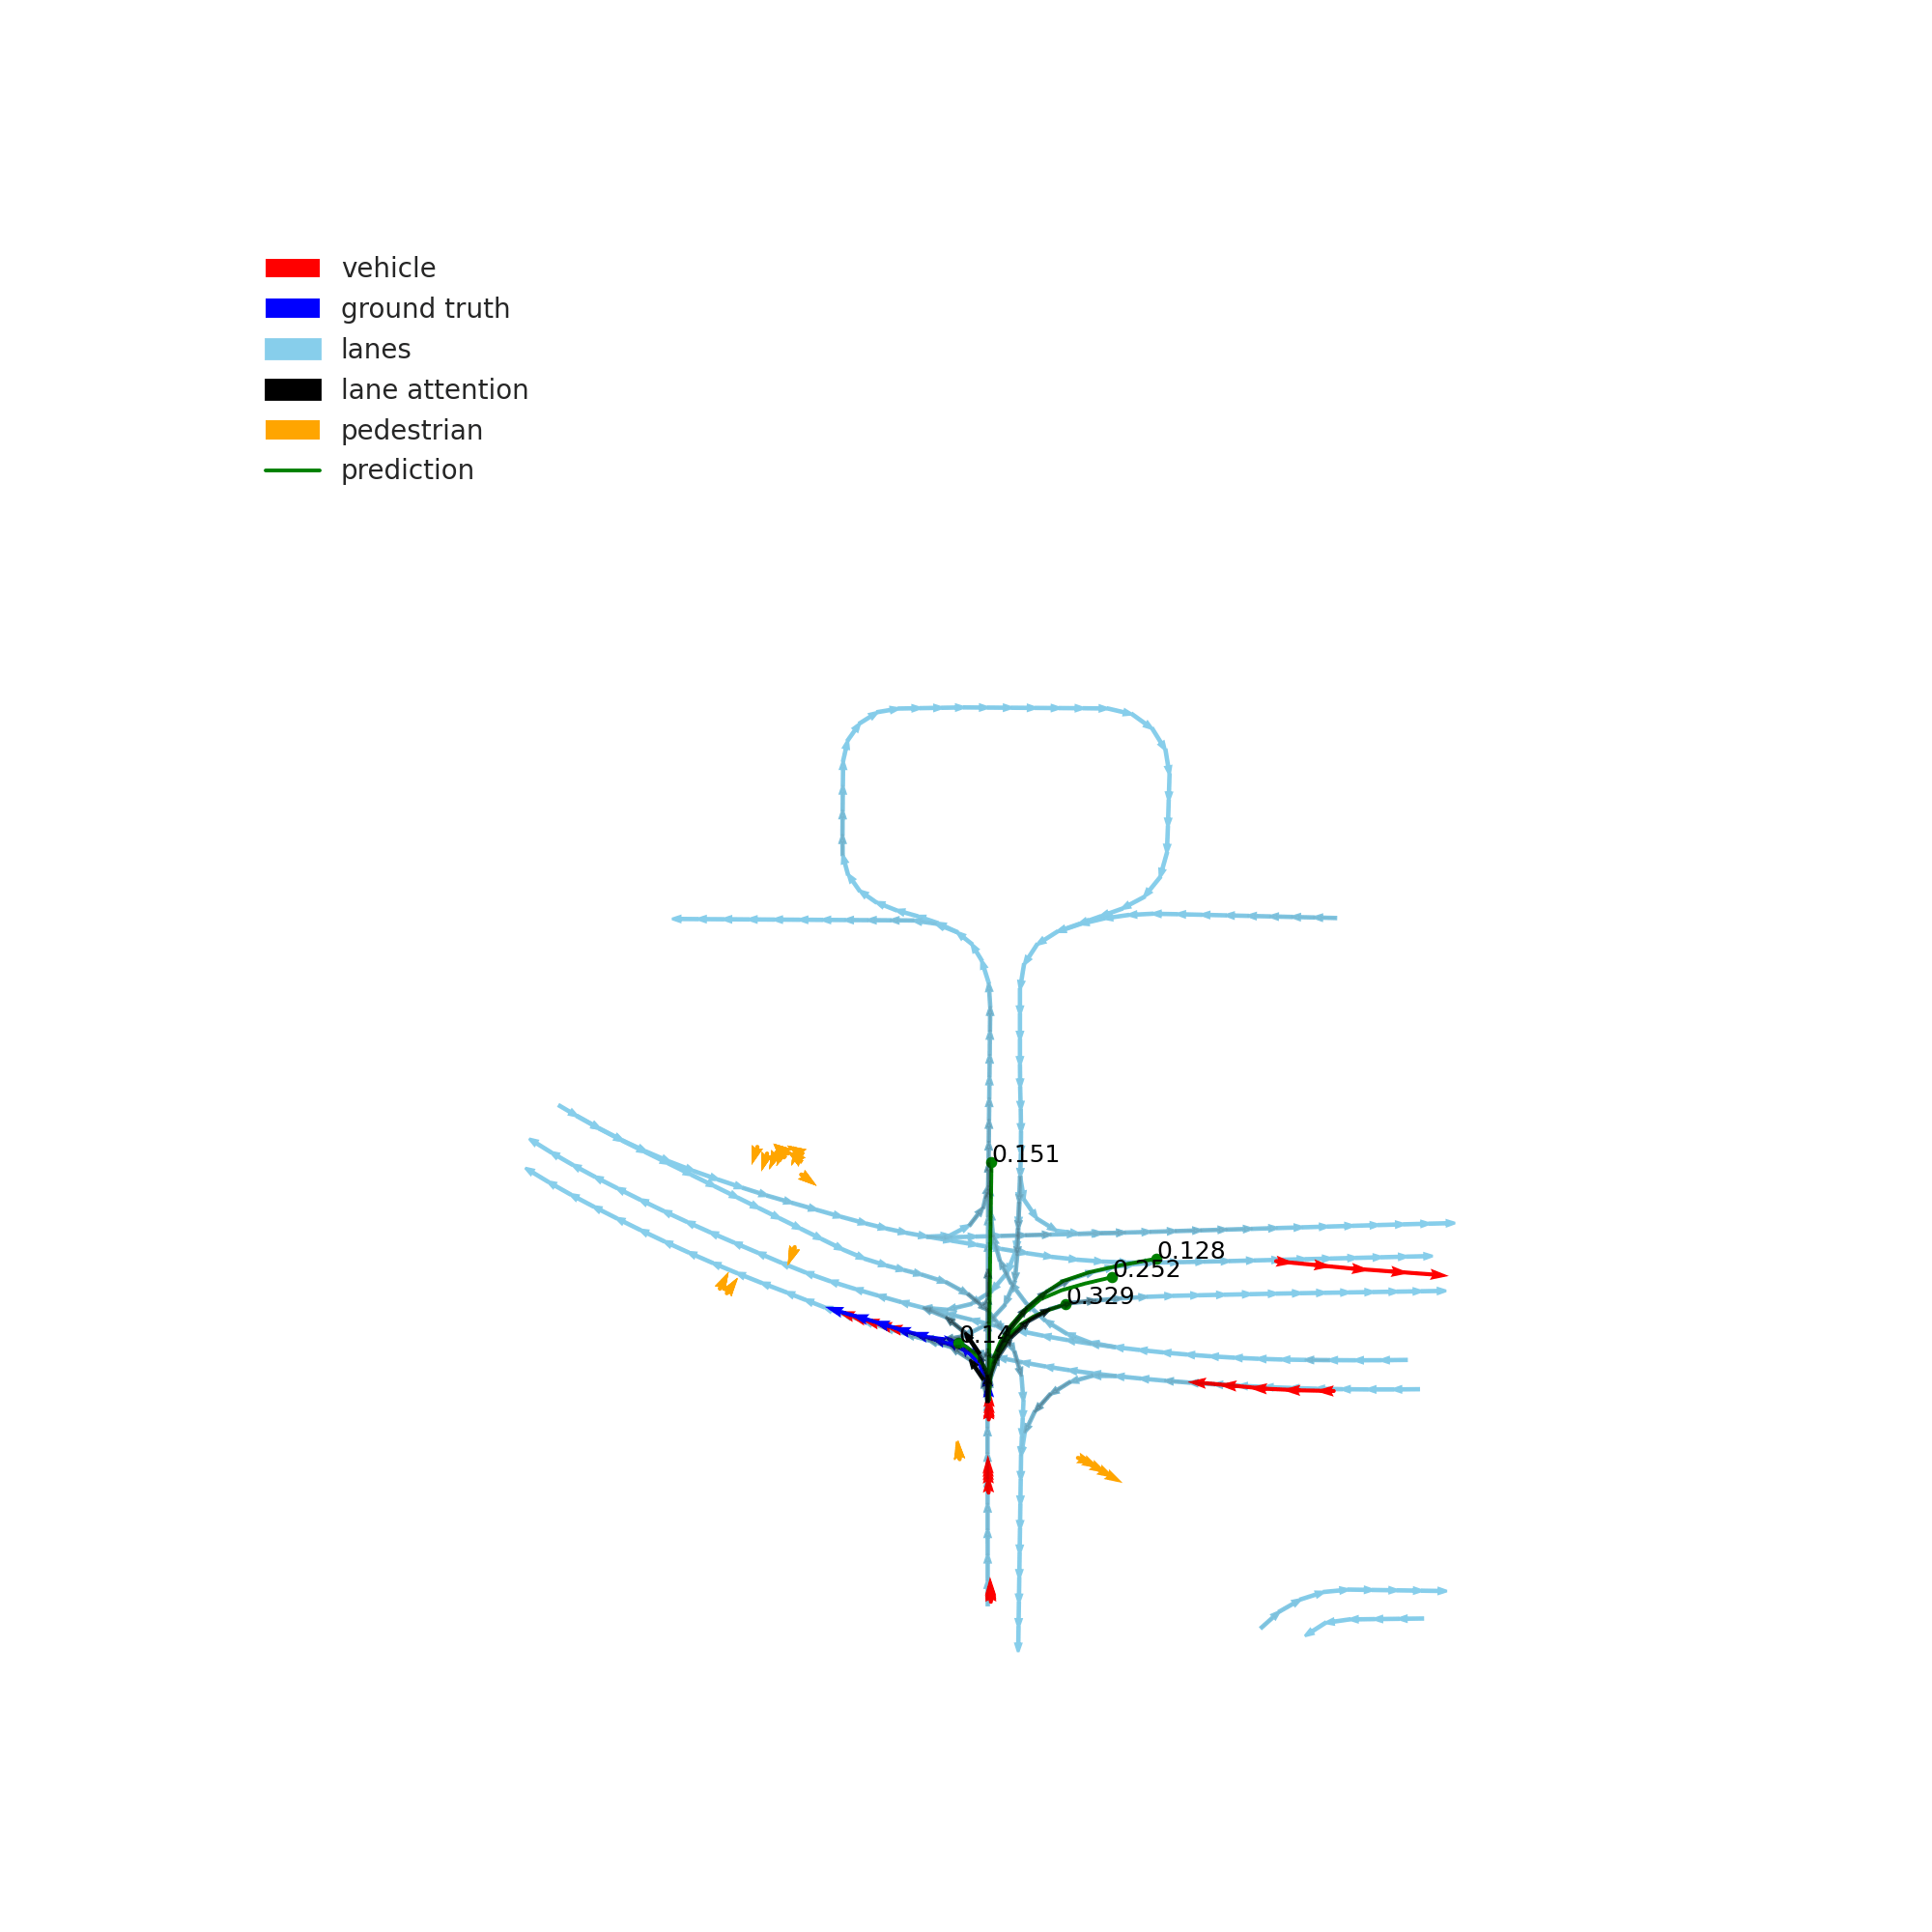
\includegraphics[height=4cm,trim={300 140 260 360},clip]{images_results/4b432f819ef44455882cb2e4d5d375ef_4809652b5d2a4ea29bbe1bbb1bacd43a_minADE5_5.72_2-min.png}
        % \caption{Final Trajectories}
    \end{subfigure}
    % \begin{subfigure}[t]{0.4\linewidth}
    %     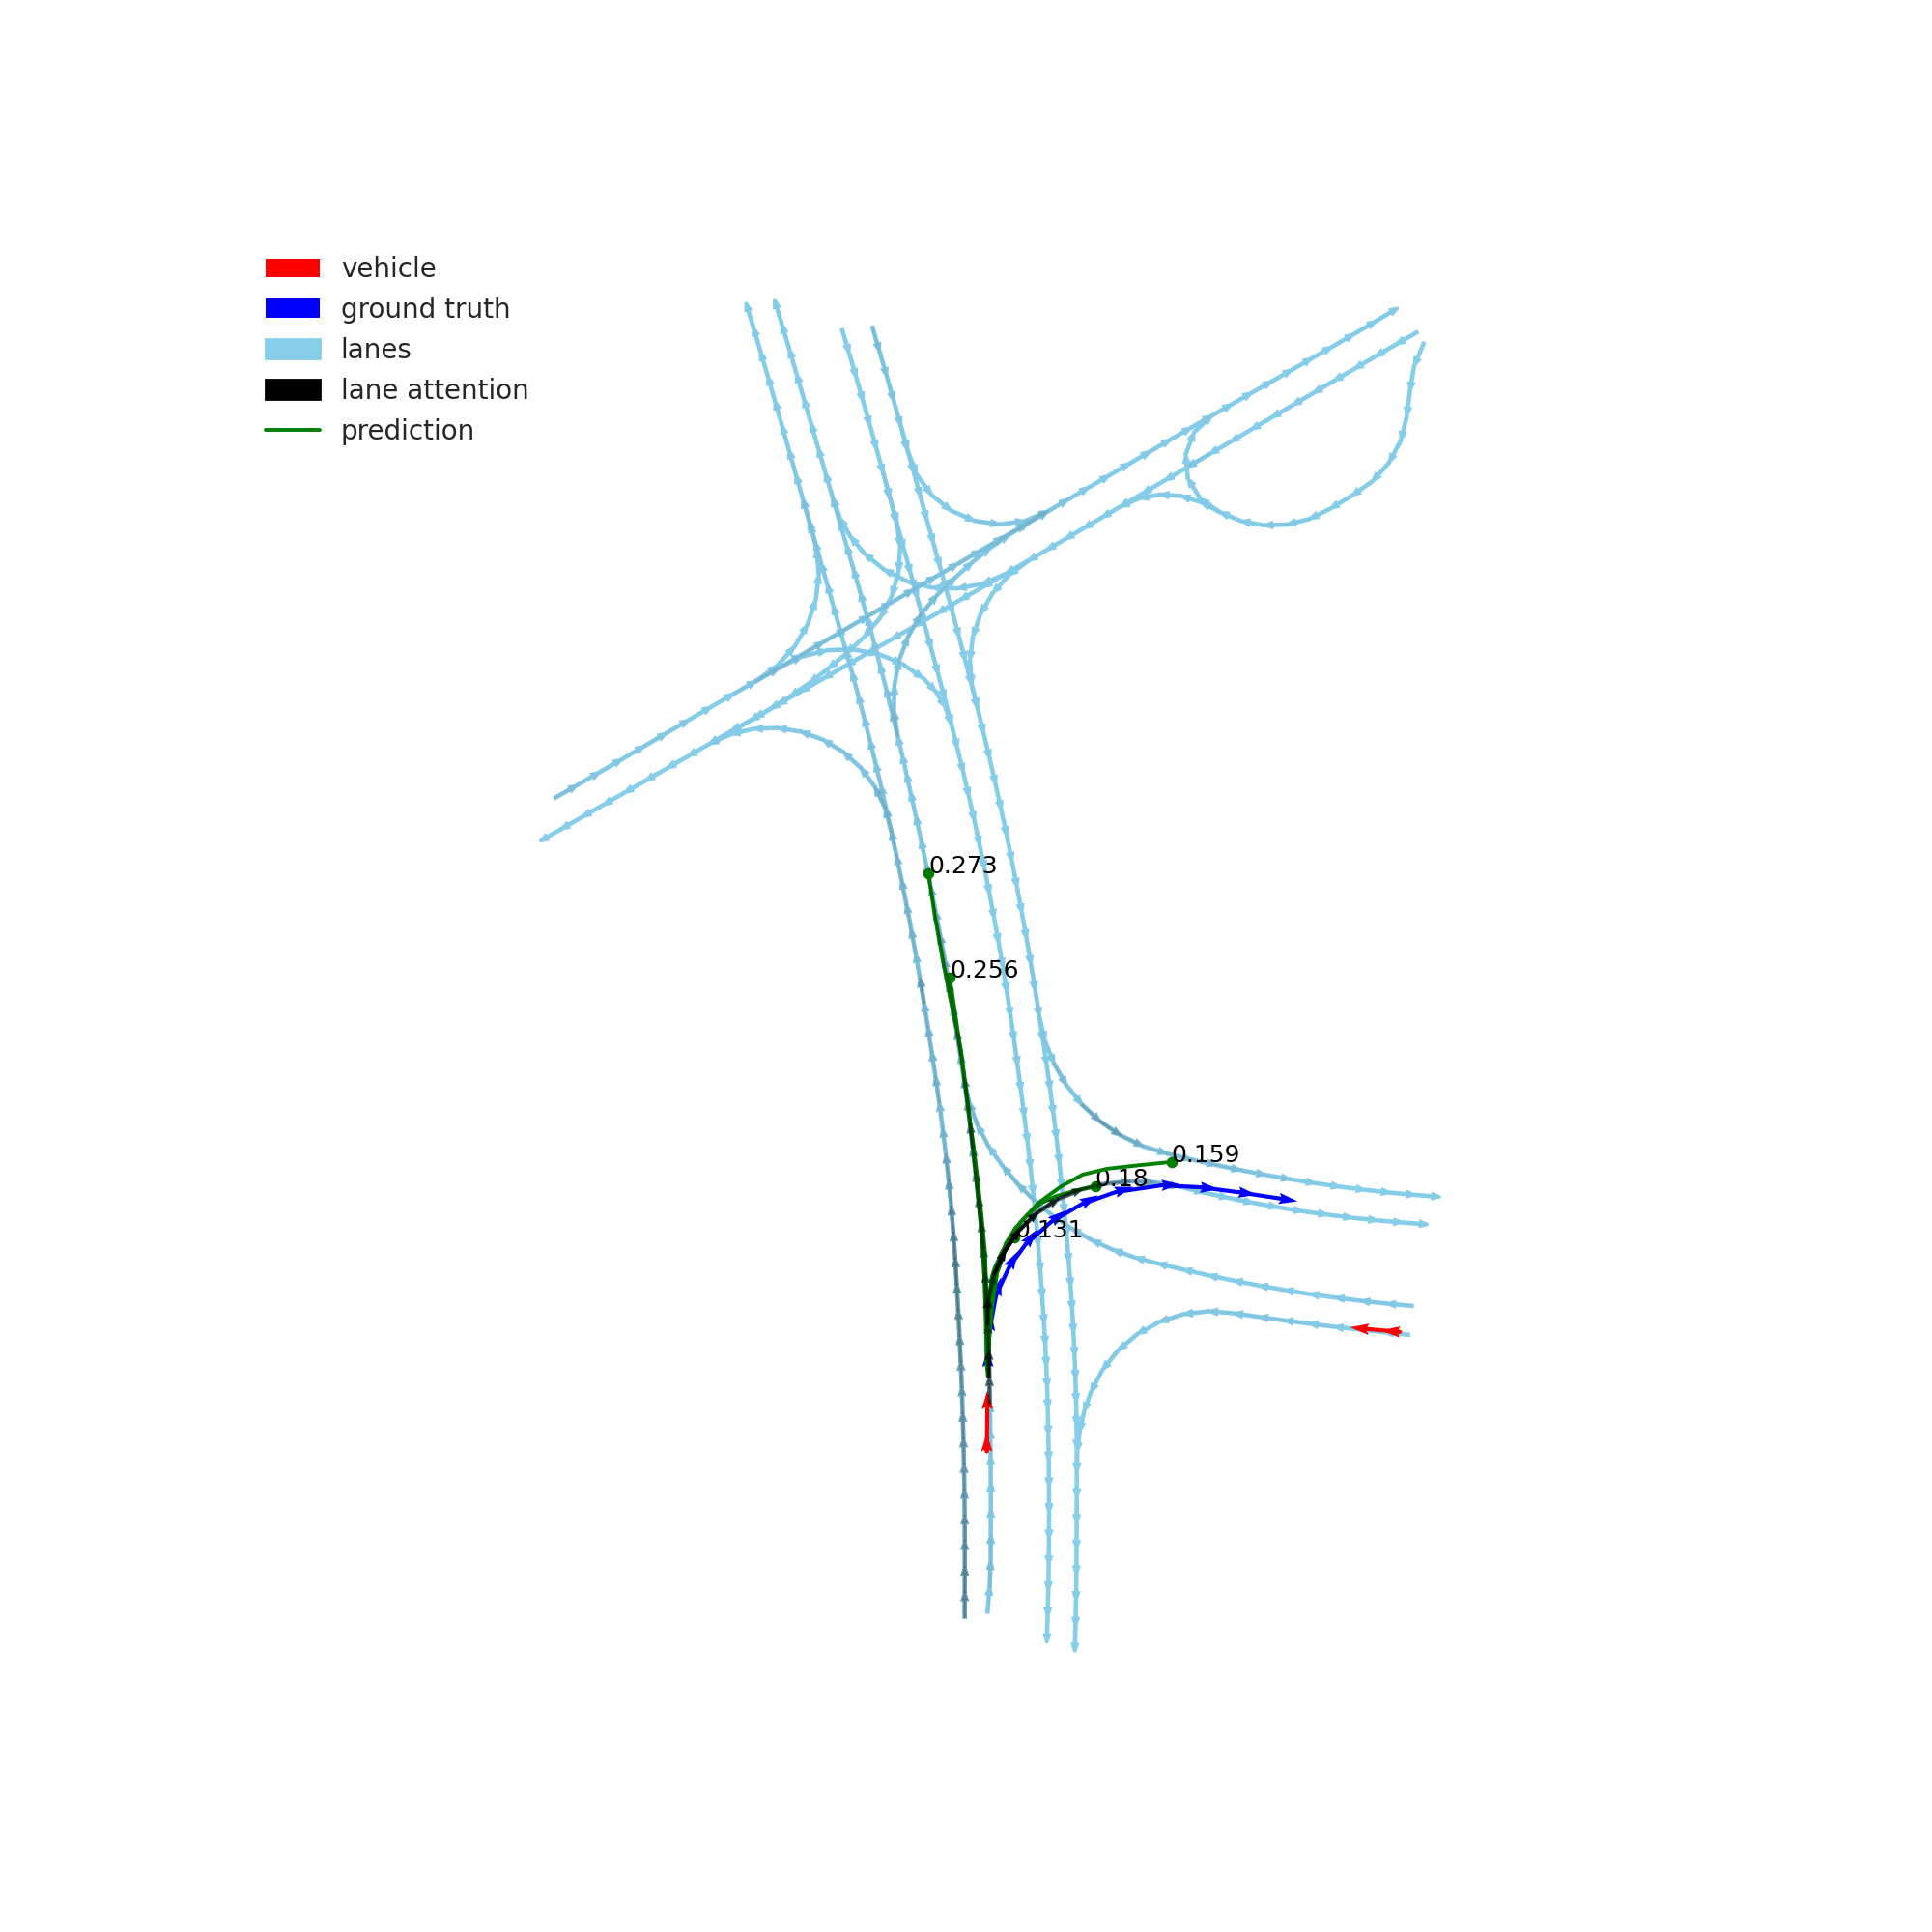
\includegraphics[height=4cm,trim={320 170 225 315},clip]{images_results/6f902cccc24d49a2b91d1d7f00047f83_6891260ad7c84844b5e74faf17303fff_minADE5_5.44_2-min.png}
    %     % \caption{Final Trajectories}
    % \end{subfigure}
    \begin{subfigure}[t]{0.4\linewidth}
        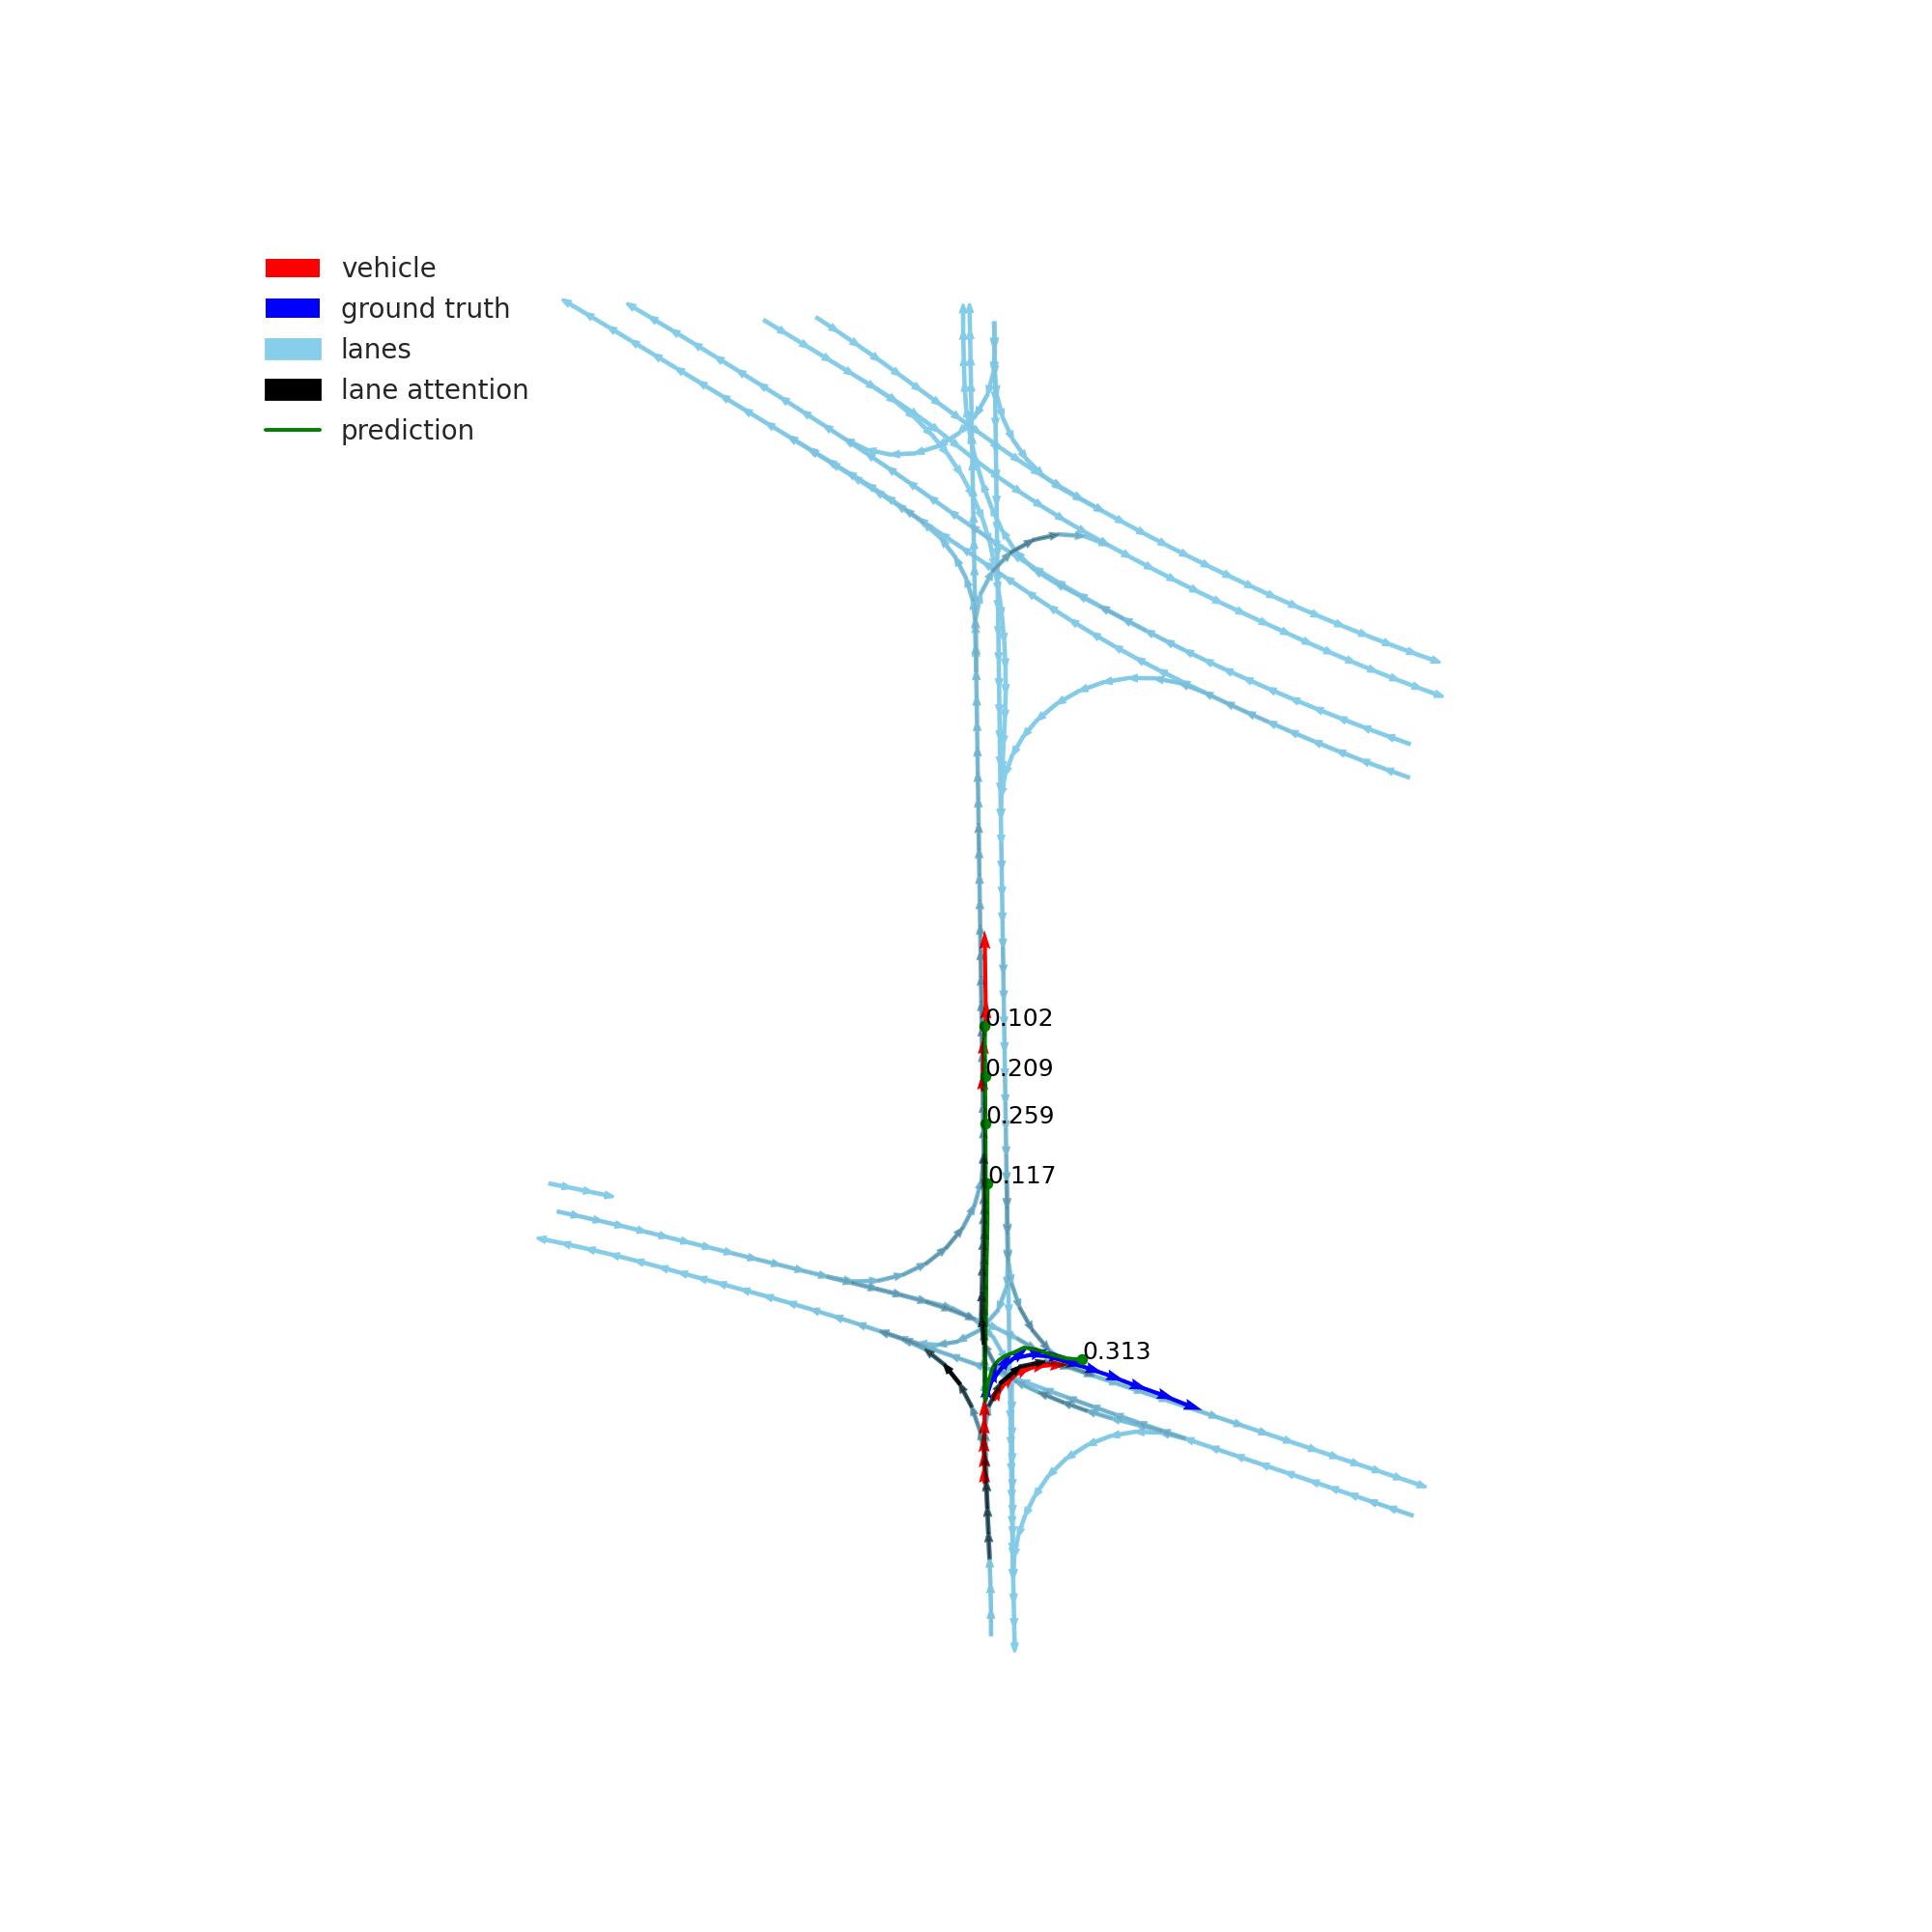
\includegraphics[height=4cm,trim={320 160 260 330},clip]{images_results/159dc0dc10134858aed2d6005da00b27_04147507f33e495f912cb64a60bb3f0d_minADE5_5.73_2-min.png}
        % \caption{Final Trajectories}
    \end{subfigure}
    \begin{tikzpicture}[remember picture,overlay]
      \node at (0, 3.3)      {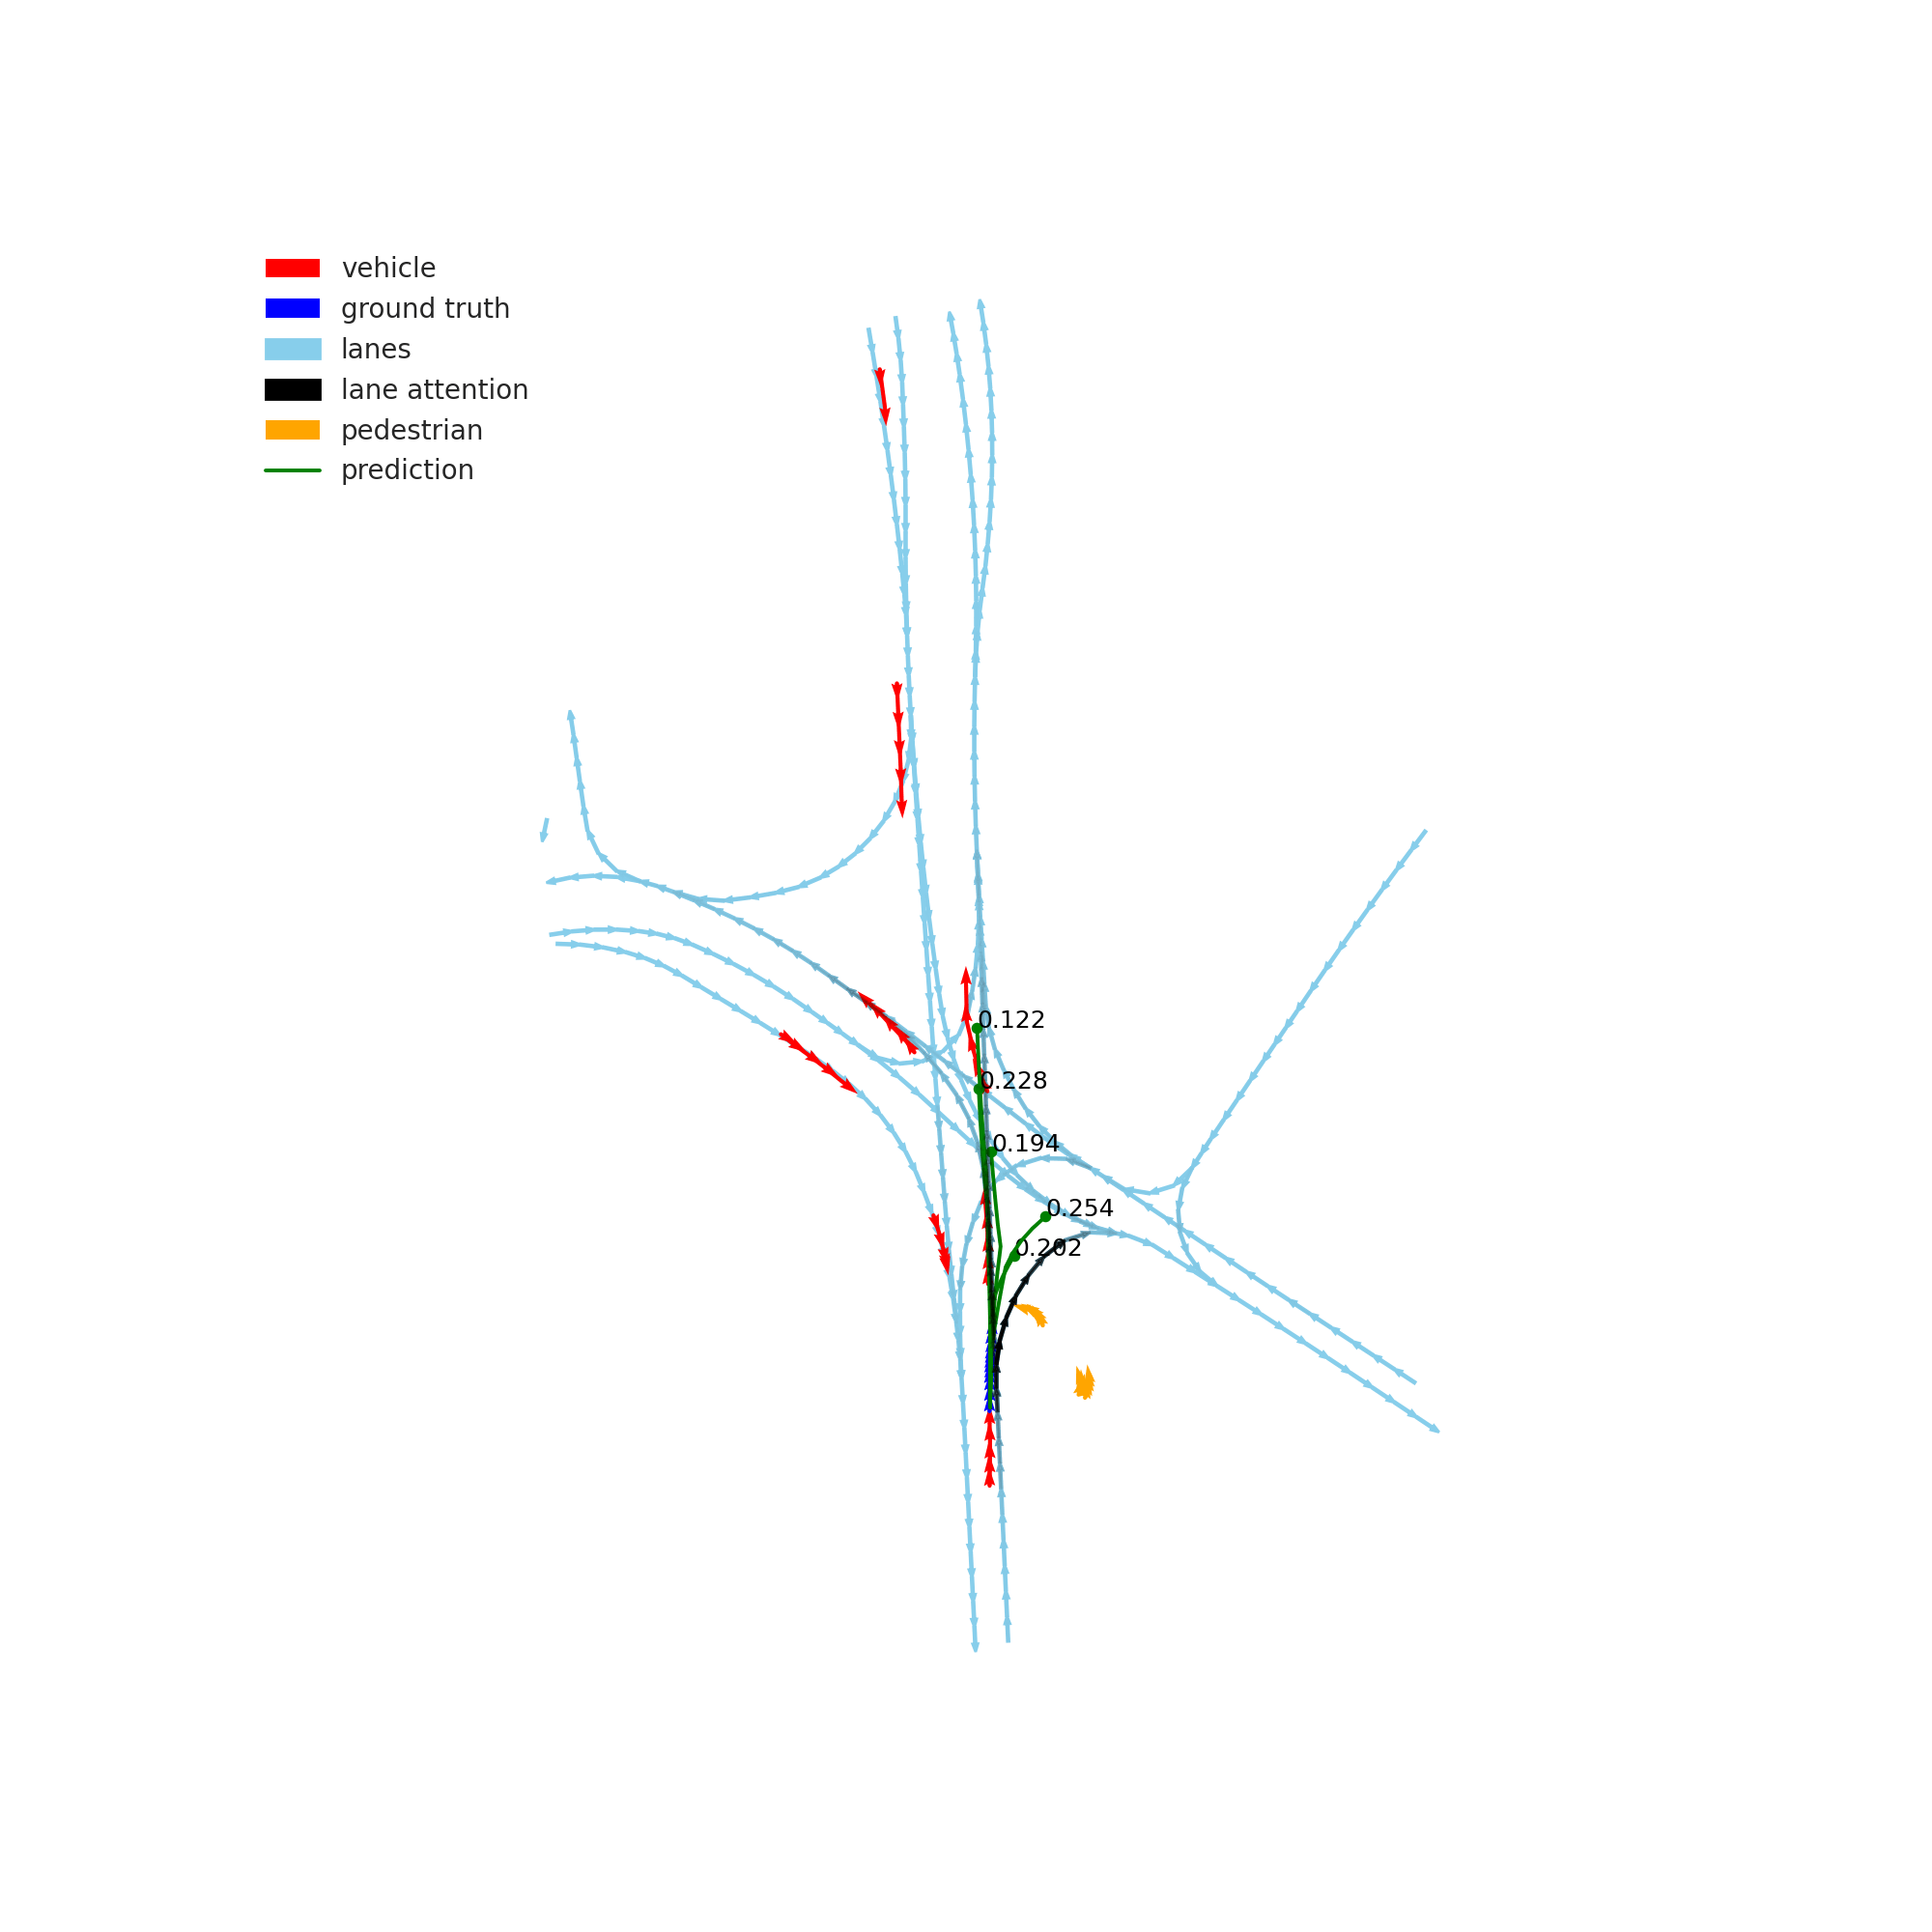
\includegraphics[width=0.23\linewidth,trim={110 500 450 85},clip]{images_results/2706cc4eb61844a1a5c7a5cb766ffc2e_37ab2d88d07846ef96d5227e9c5a15d7_minADE5_5.01_0-min.png}};
    \end{tikzpicture}
    \caption{An illustration of predicted trajectories (green) with mode probabilities for the target agent at the final output layer. These samples are selected out of the 100 worst predictions based on minADE\textsubscript{5}.}
    \label{fig:nuScenes_worst}    
\end{figure}

We also test the generalization capability of LMFormer on the Deep Scenario dataset \cite{lu2023deepscenario}. To this end, we train the network on 55,000 training samples, generated from four different intersections' recordings ('Unparalleled Frankfurt', 'Trendy Renningen', Fortunate Karlsruhe', 'Stunning Stuttgart') in the dataset. We conducted the qualitative testing for this model checkpoint on the samples of unobserved intersections during training (refer Figure \ref{fig:cross_data_qual}). We observe that in certain cases, LMFormer fails to predict all plausible trajectories. We hypothesize that this limitation is due to an unbalanced data distribution, where some maneuvers occur less frequently in the training data. This suggests that additional mechanisms, such as explicit trajectory diversity constraints or targeted data augmentation, may be required to improve the robustness of multimodal prediction, but we leave these improvements for future work.

\begin{figure}
    \centering
    \begin{subfigure}[t]{0.3\linewidth}
        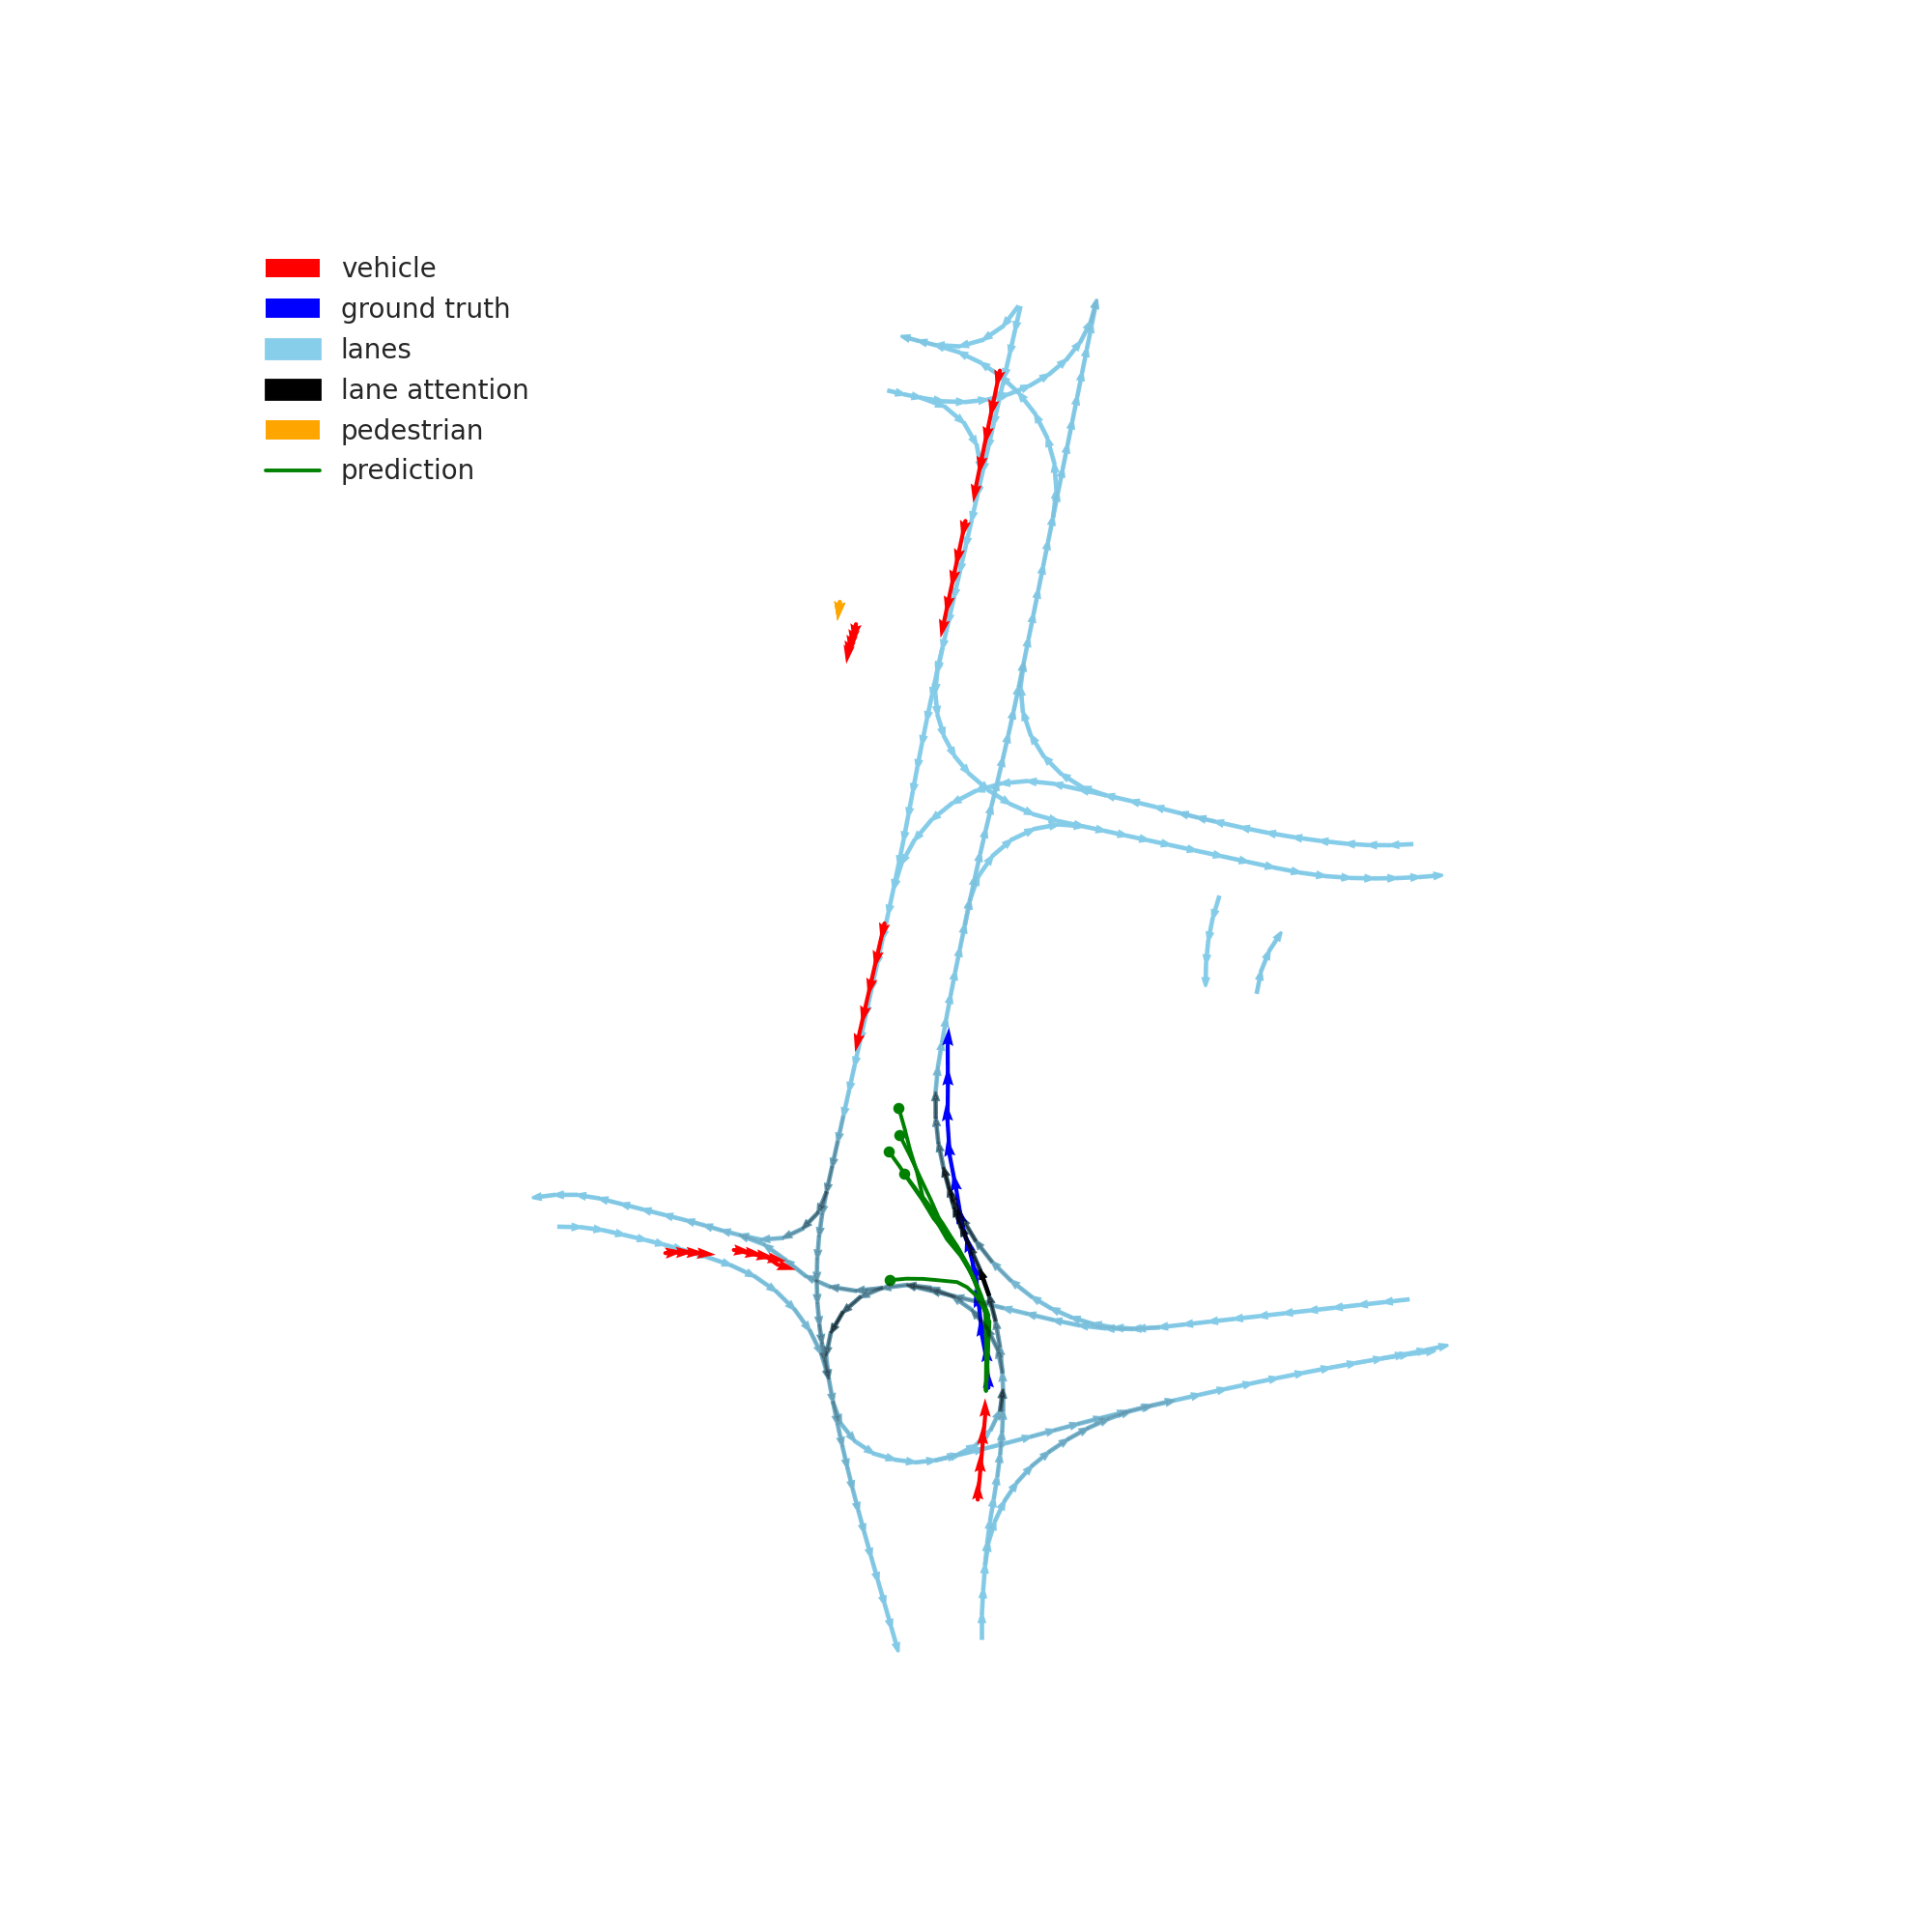
\includegraphics[height=3cm,trim={280 160 300 370},clip]{images_results/56d0094604014dee90a4dfb6f861f4e6_80e84ccf181a428e939af2fbde7d4211_0-min.png}
    \end{subfigure}
    \begin{subfigure}[t]{0.3\linewidth}
        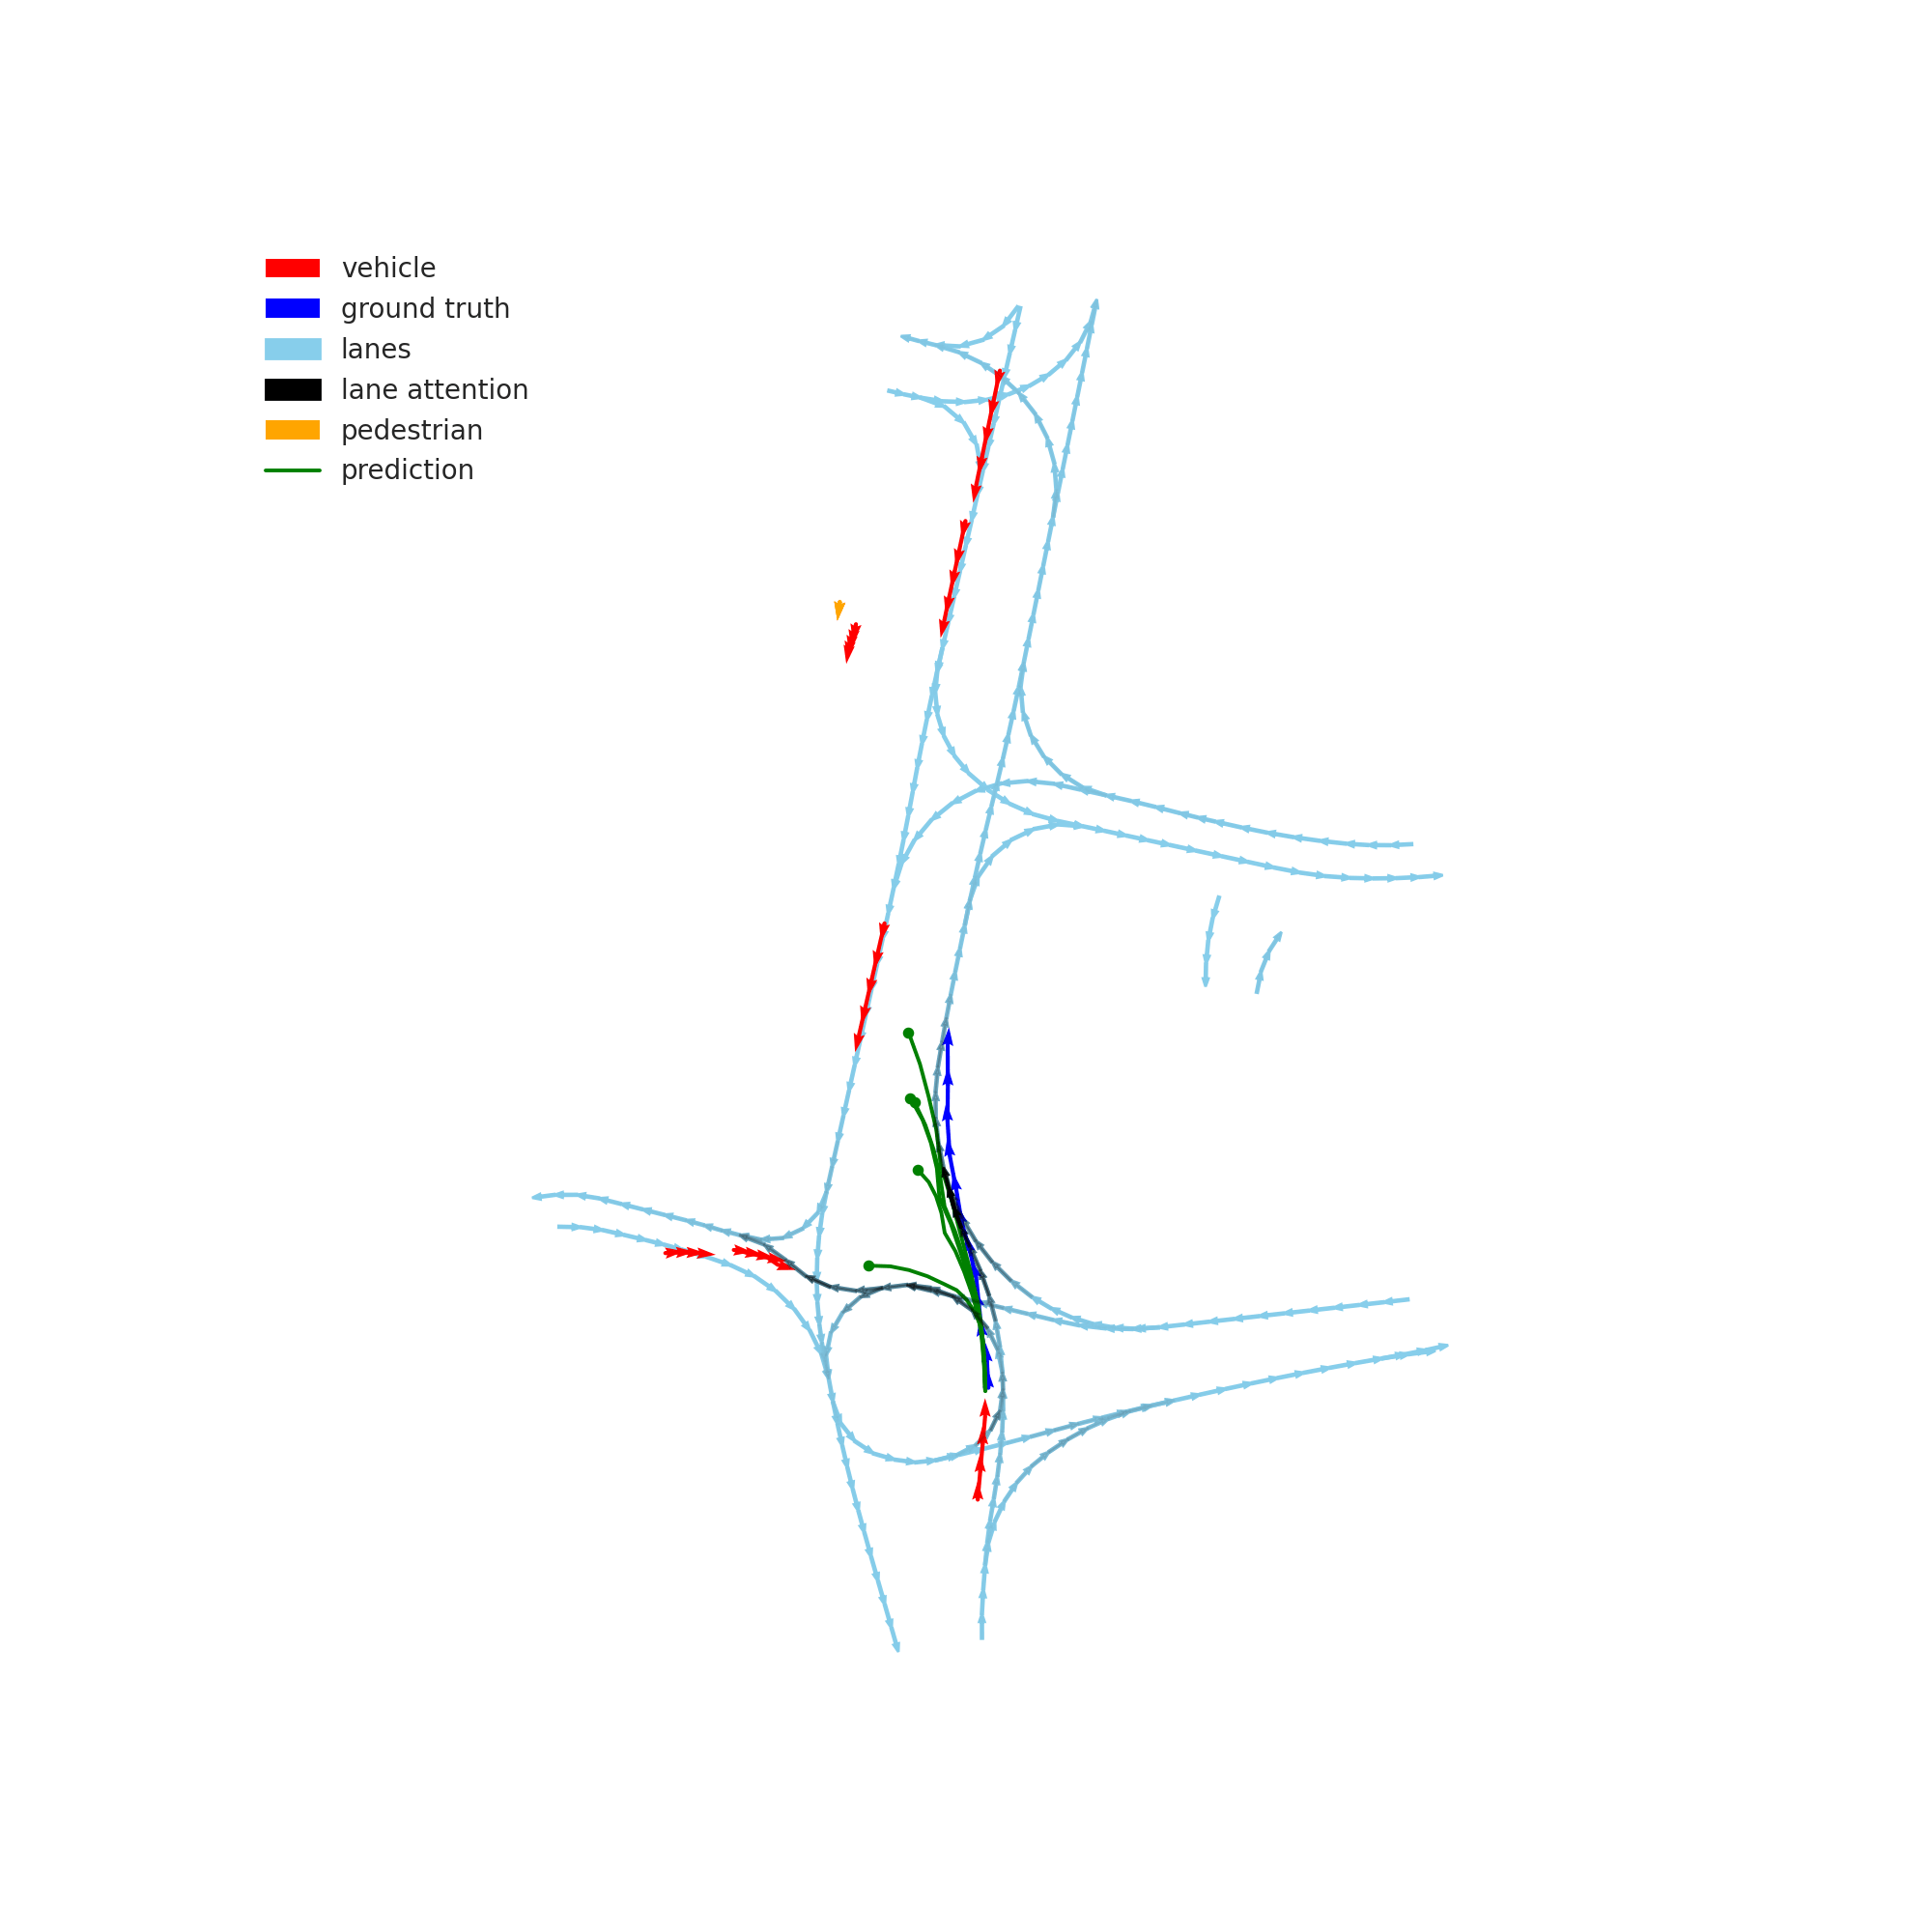
\includegraphics[height=3cm,trim={280 160 300 370},clip]{images_results/56d0094604014dee90a4dfb6f861f4e6_80e84ccf181a428e939af2fbde7d4211_1-min.png}
    \end{subfigure}
    \begin{subfigure}[t]{0.3\linewidth}
        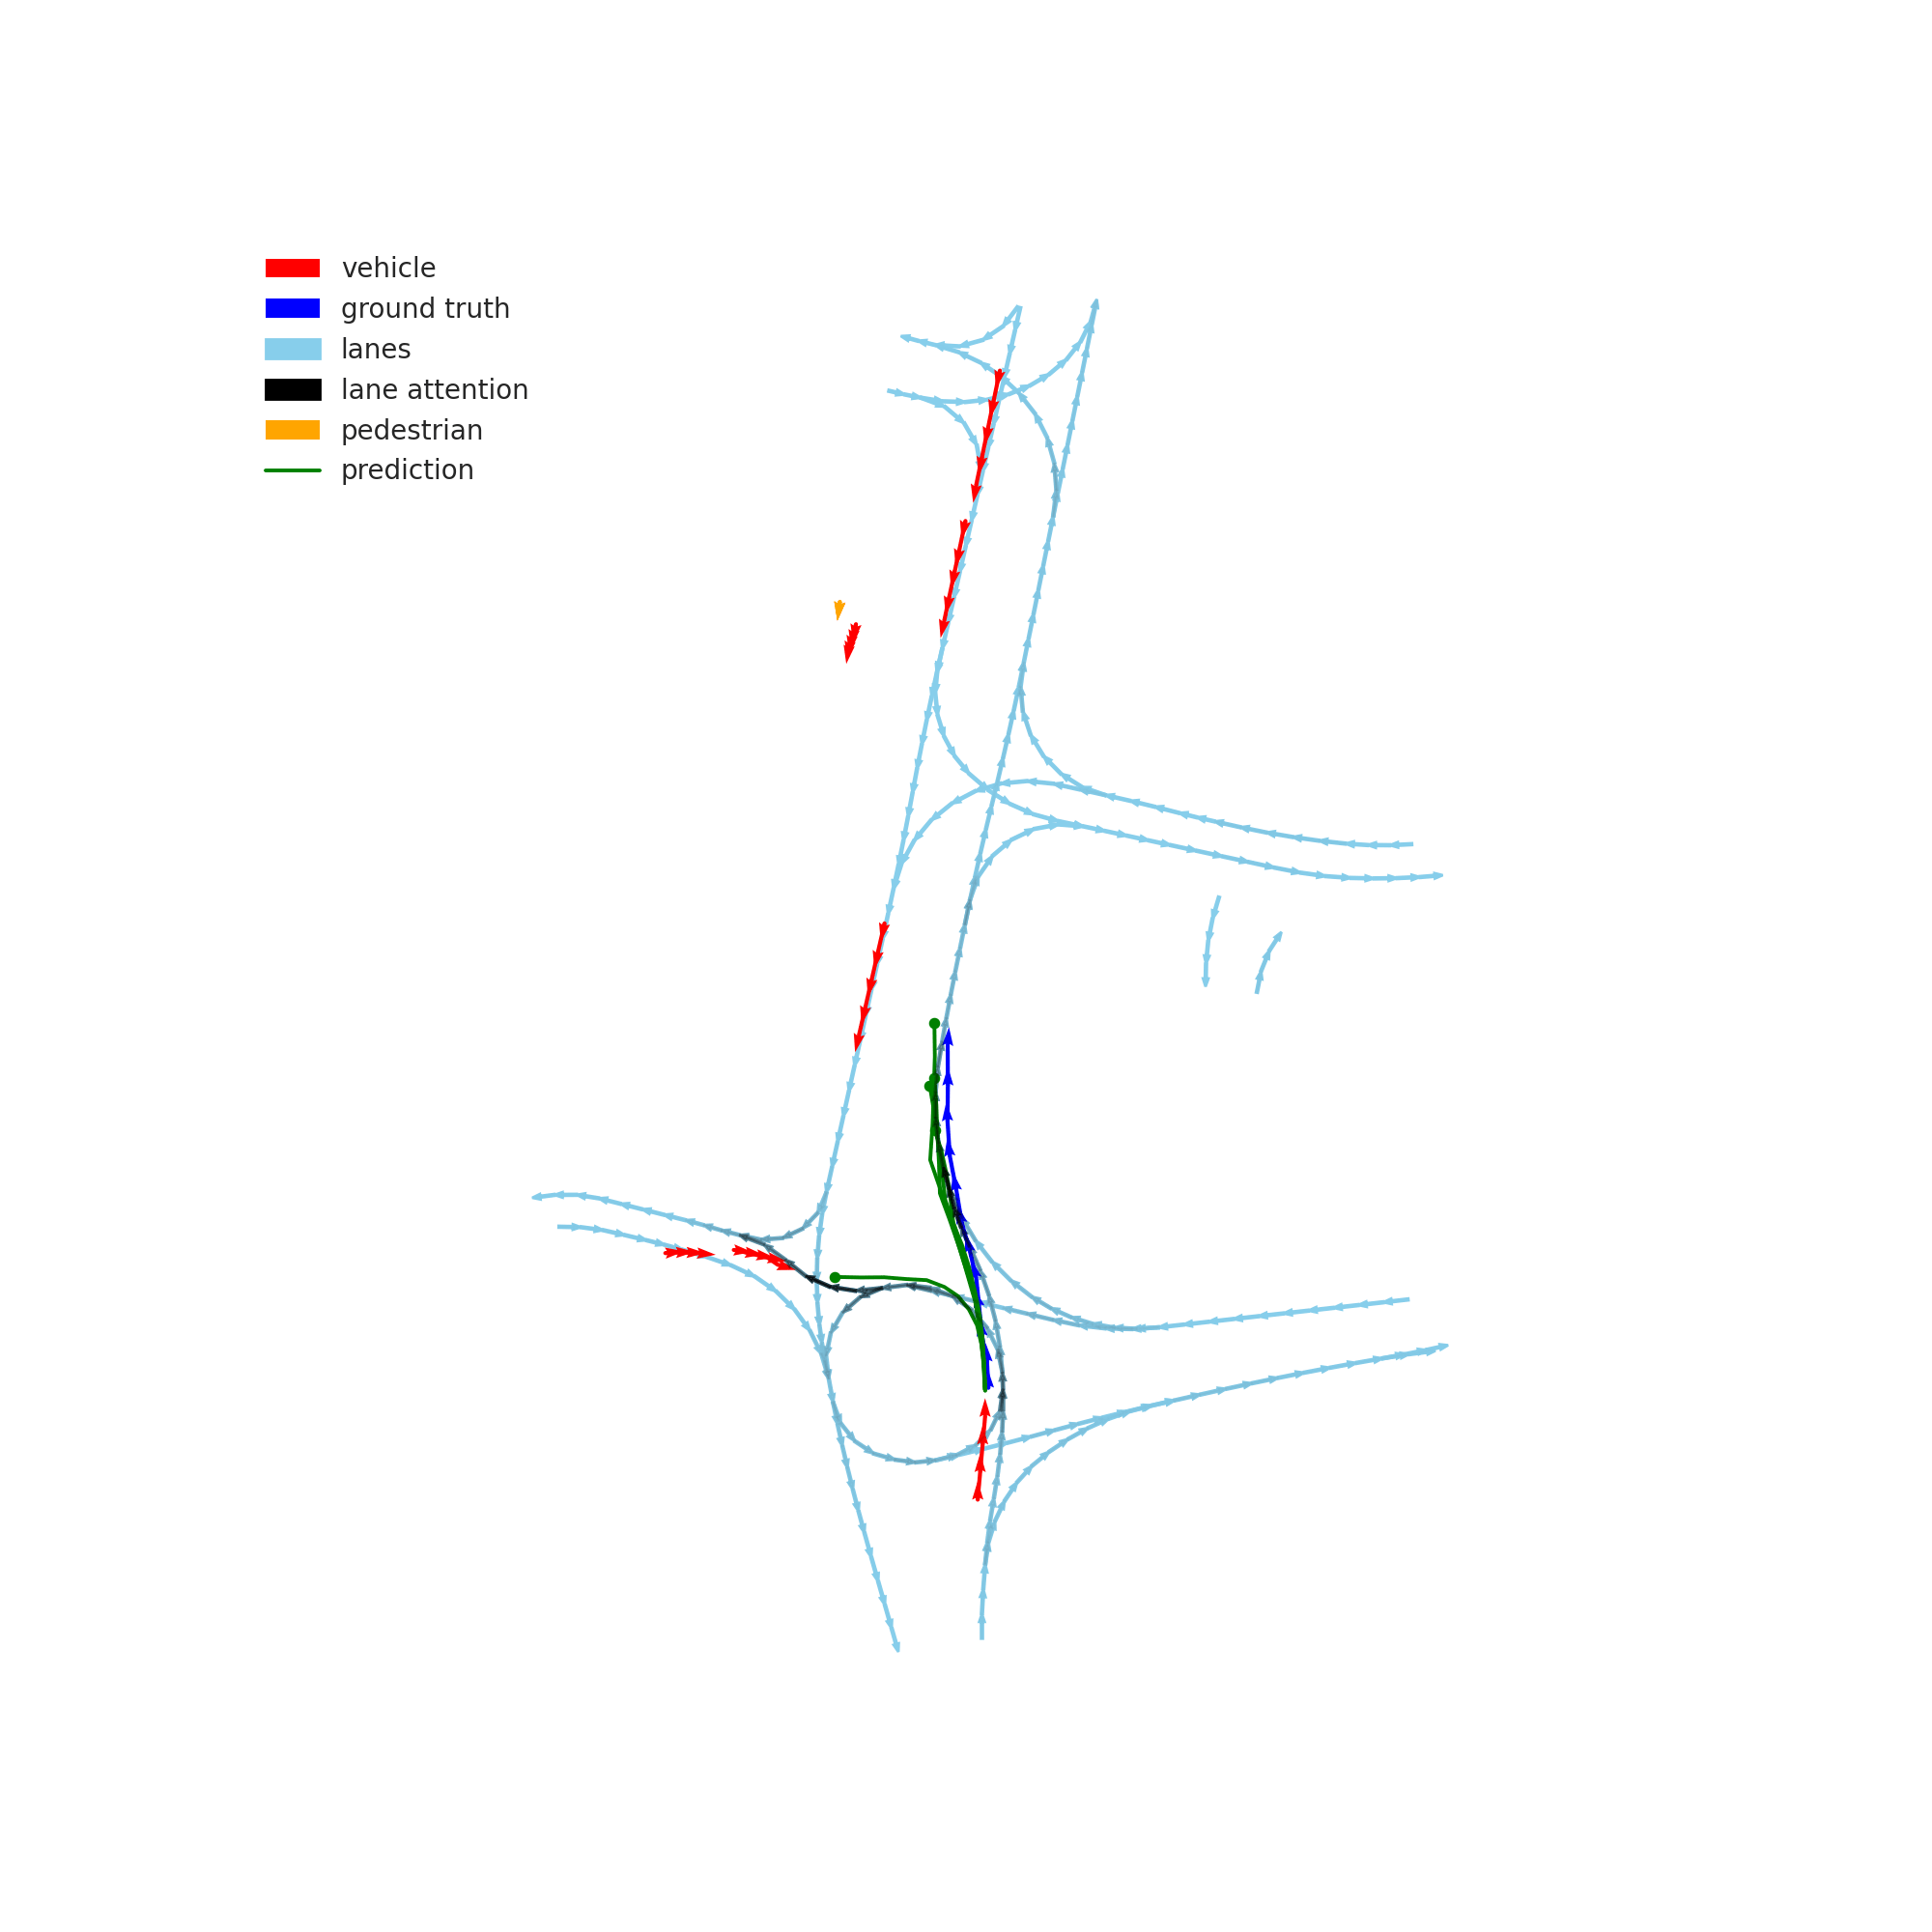
\includegraphics[height=3cm,trim={280 160 300 370},clip]{images_results/56d0094604014dee90a4dfb6f861f4e6_80e84ccf181a428e939af2fbde7d4211_2-min.png}
    \end{subfigure}
    \begin{subfigure}[t]{0.3\linewidth}
        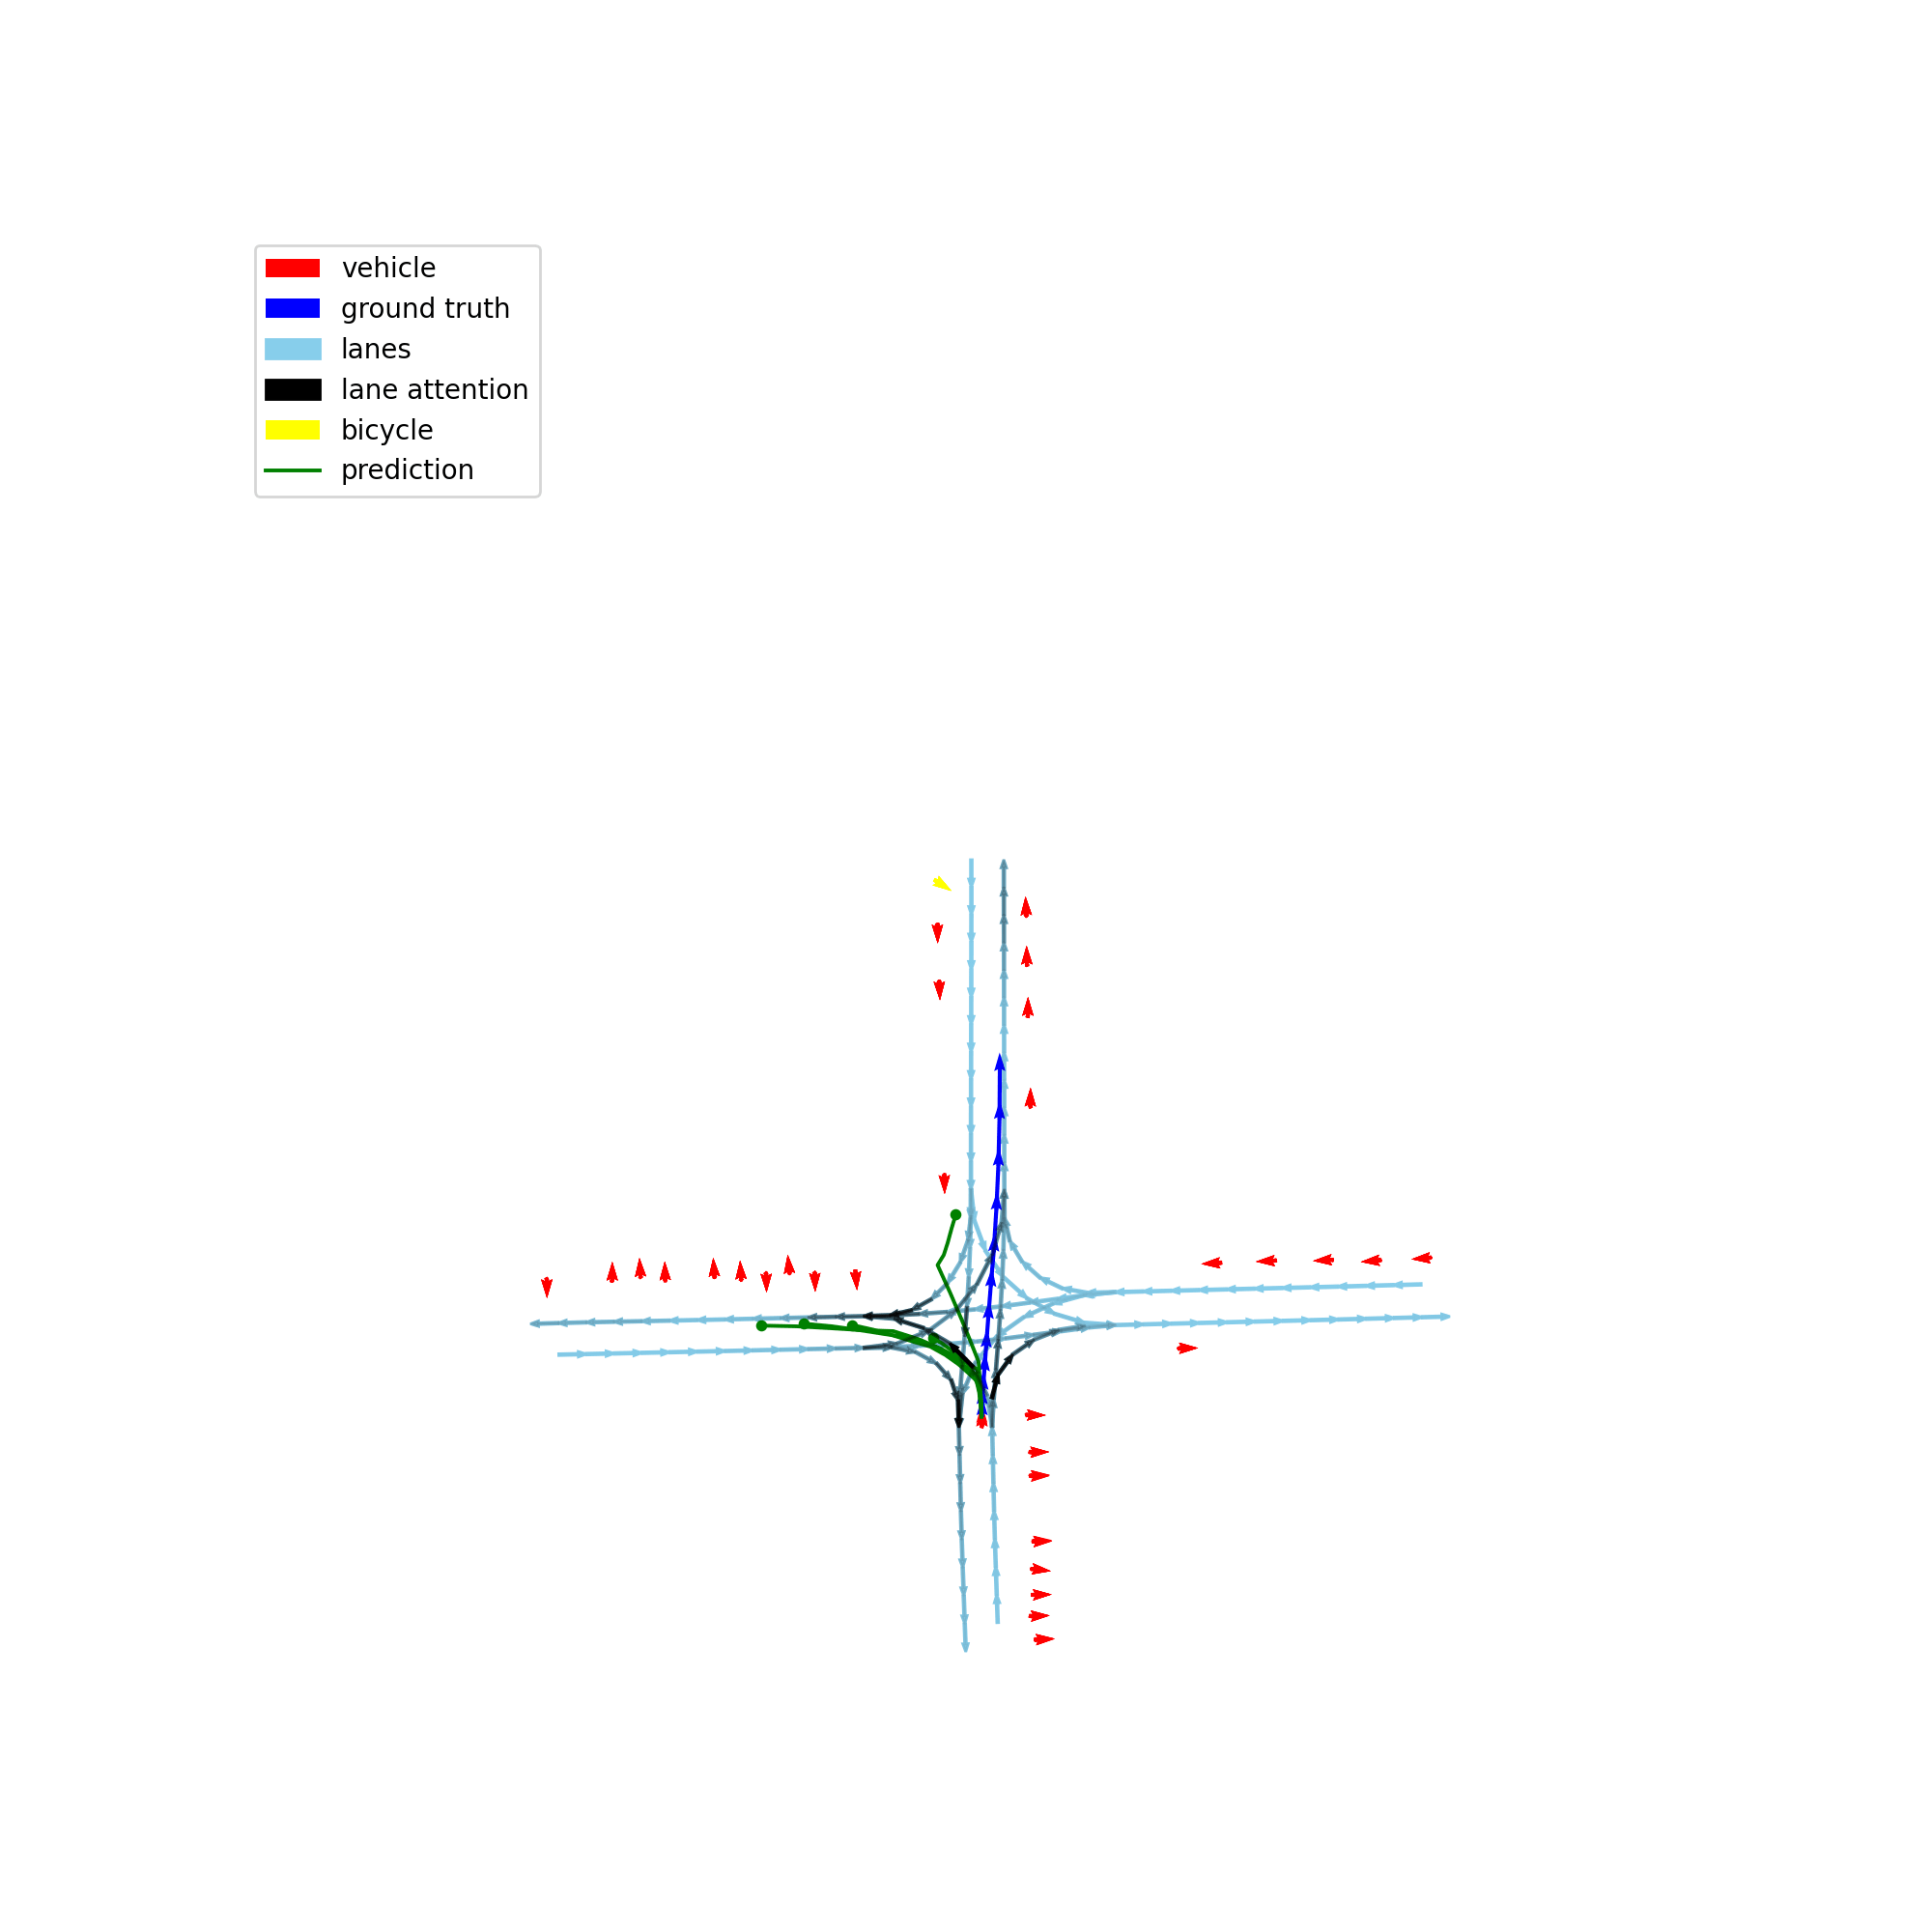
\includegraphics[height=3cm,trim={280 170 300 380},clip]{images_results/1337_minADE5_9.3_0-min.png}
        \caption{Initial}
    \end{subfigure}
    \begin{subfigure}[t]{0.3\linewidth}
        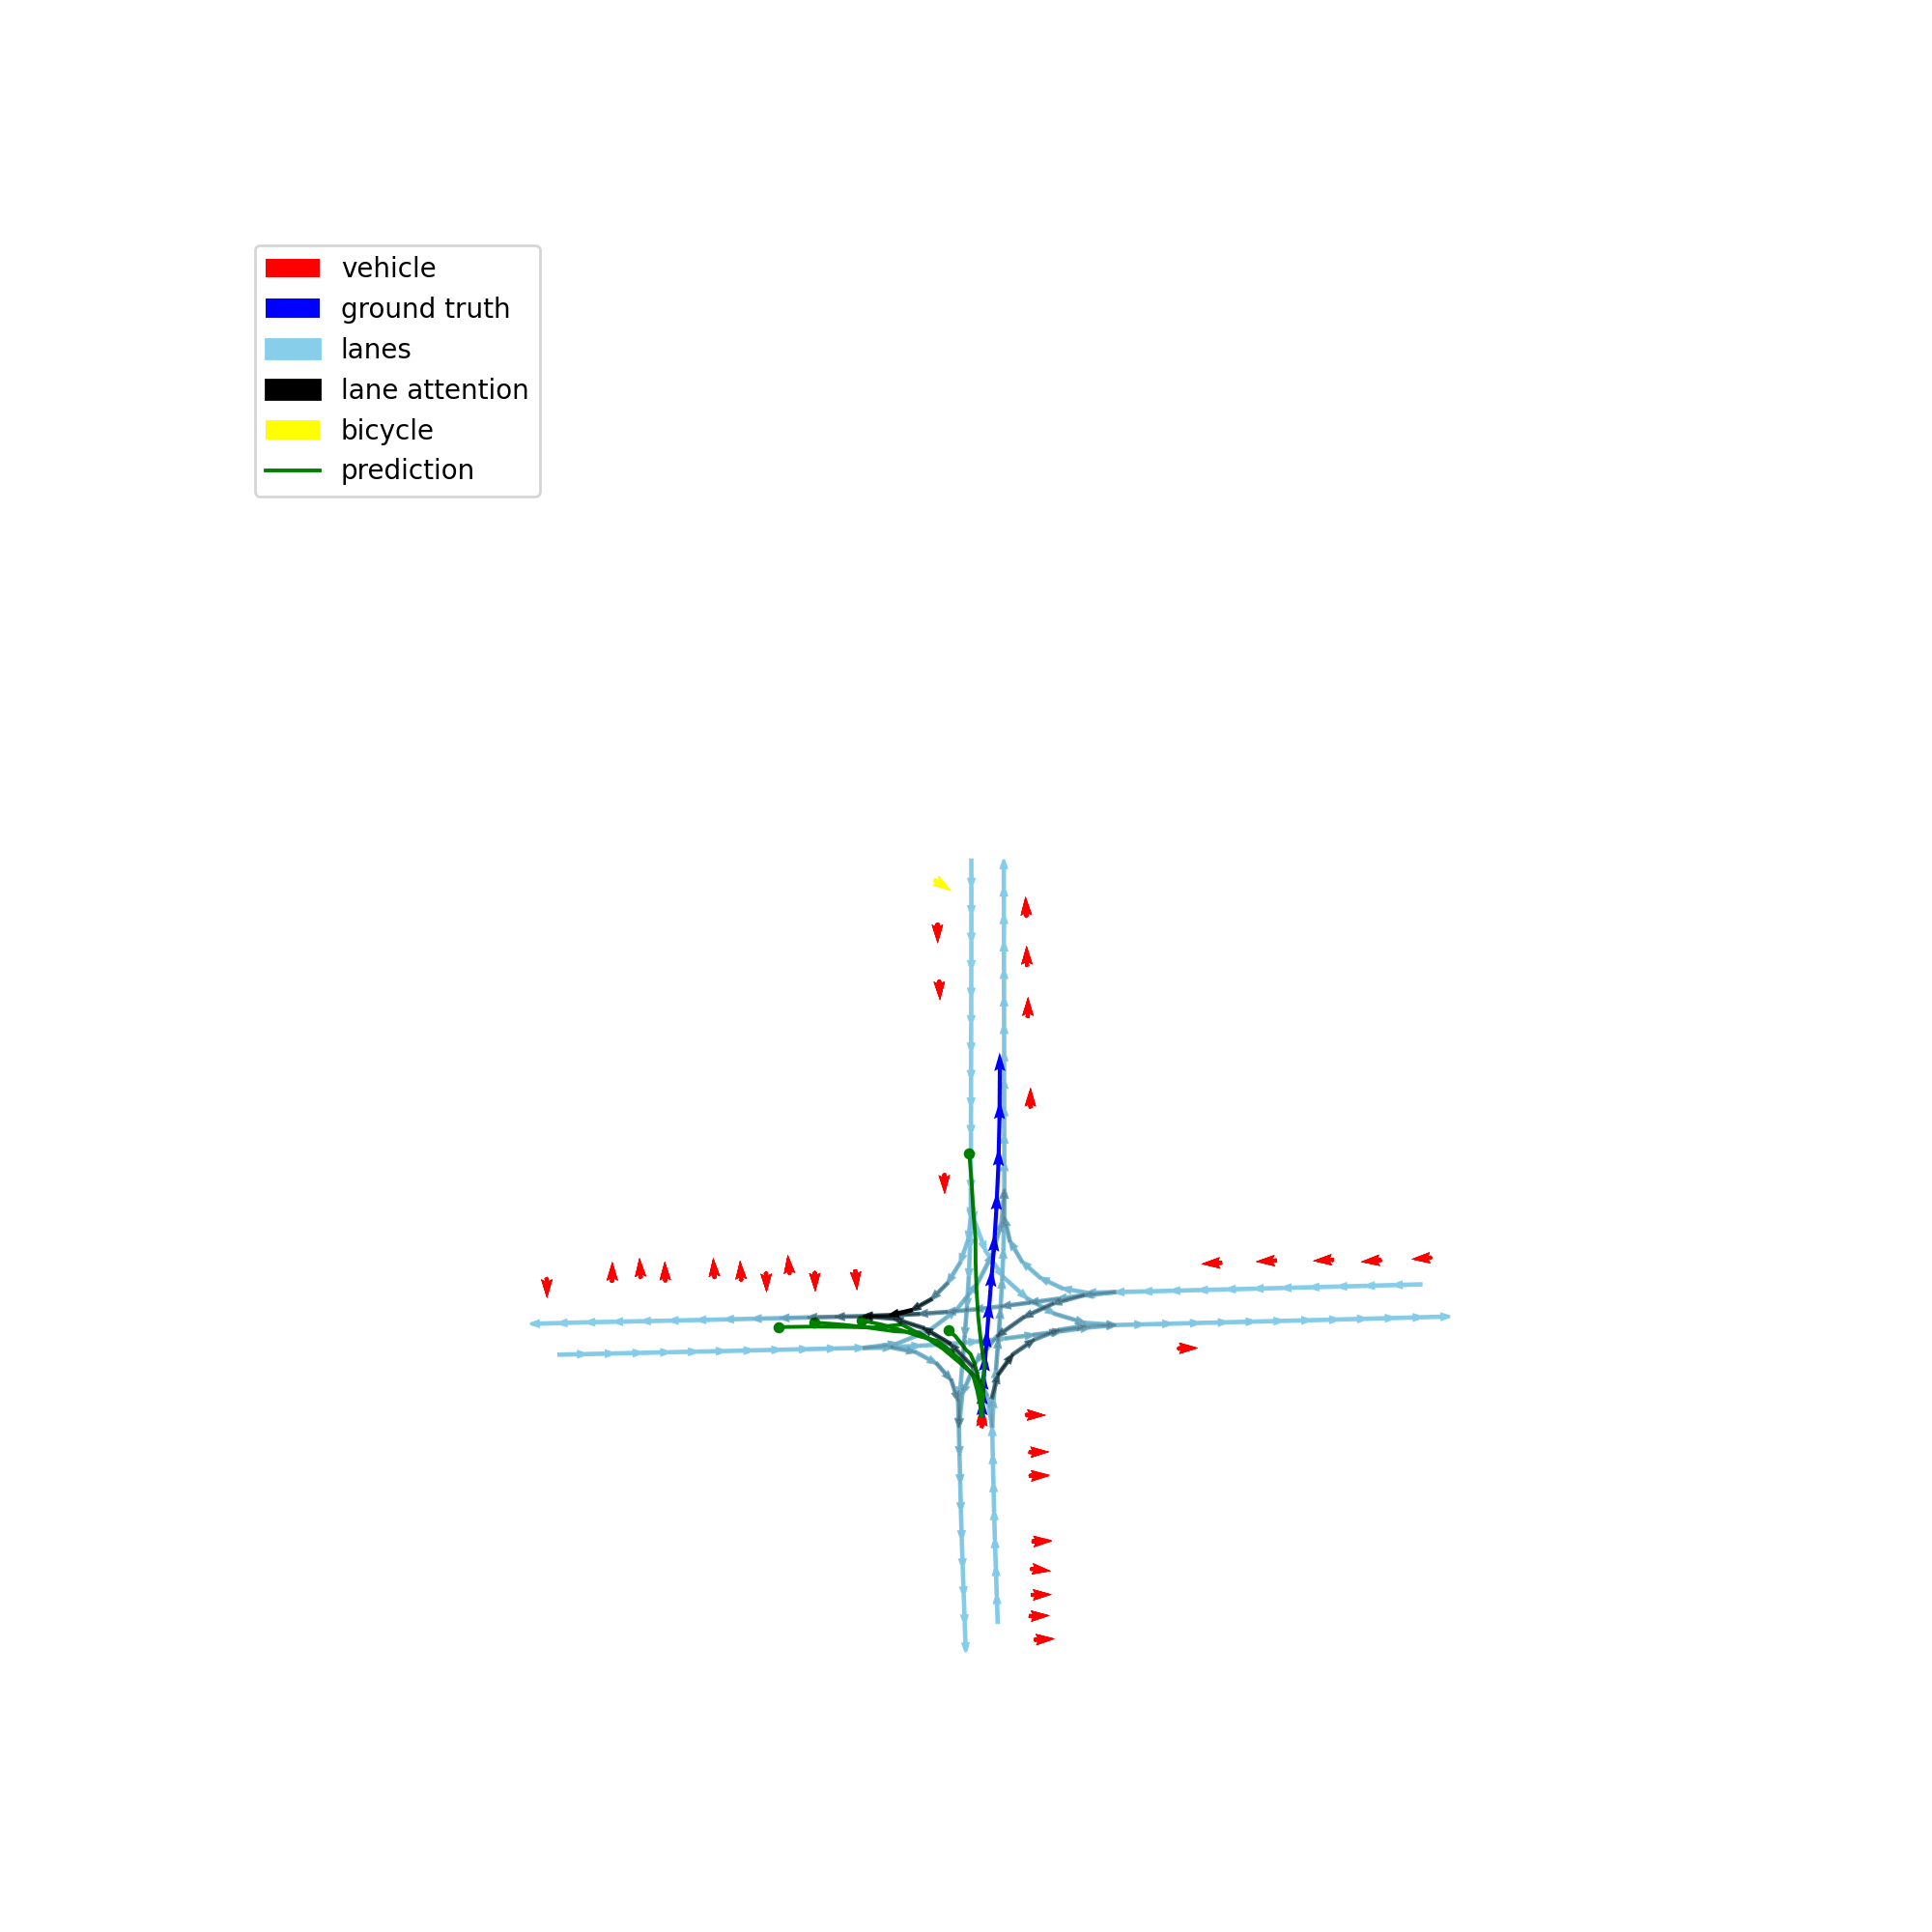
\includegraphics[height=3cm,trim={280 170 300 380},clip]{images_results/1337_minADE5_9.3_1-min.png}
        \caption{Refinement}
    \end{subfigure}
    \begin{subfigure}[t]{0.3\linewidth}
        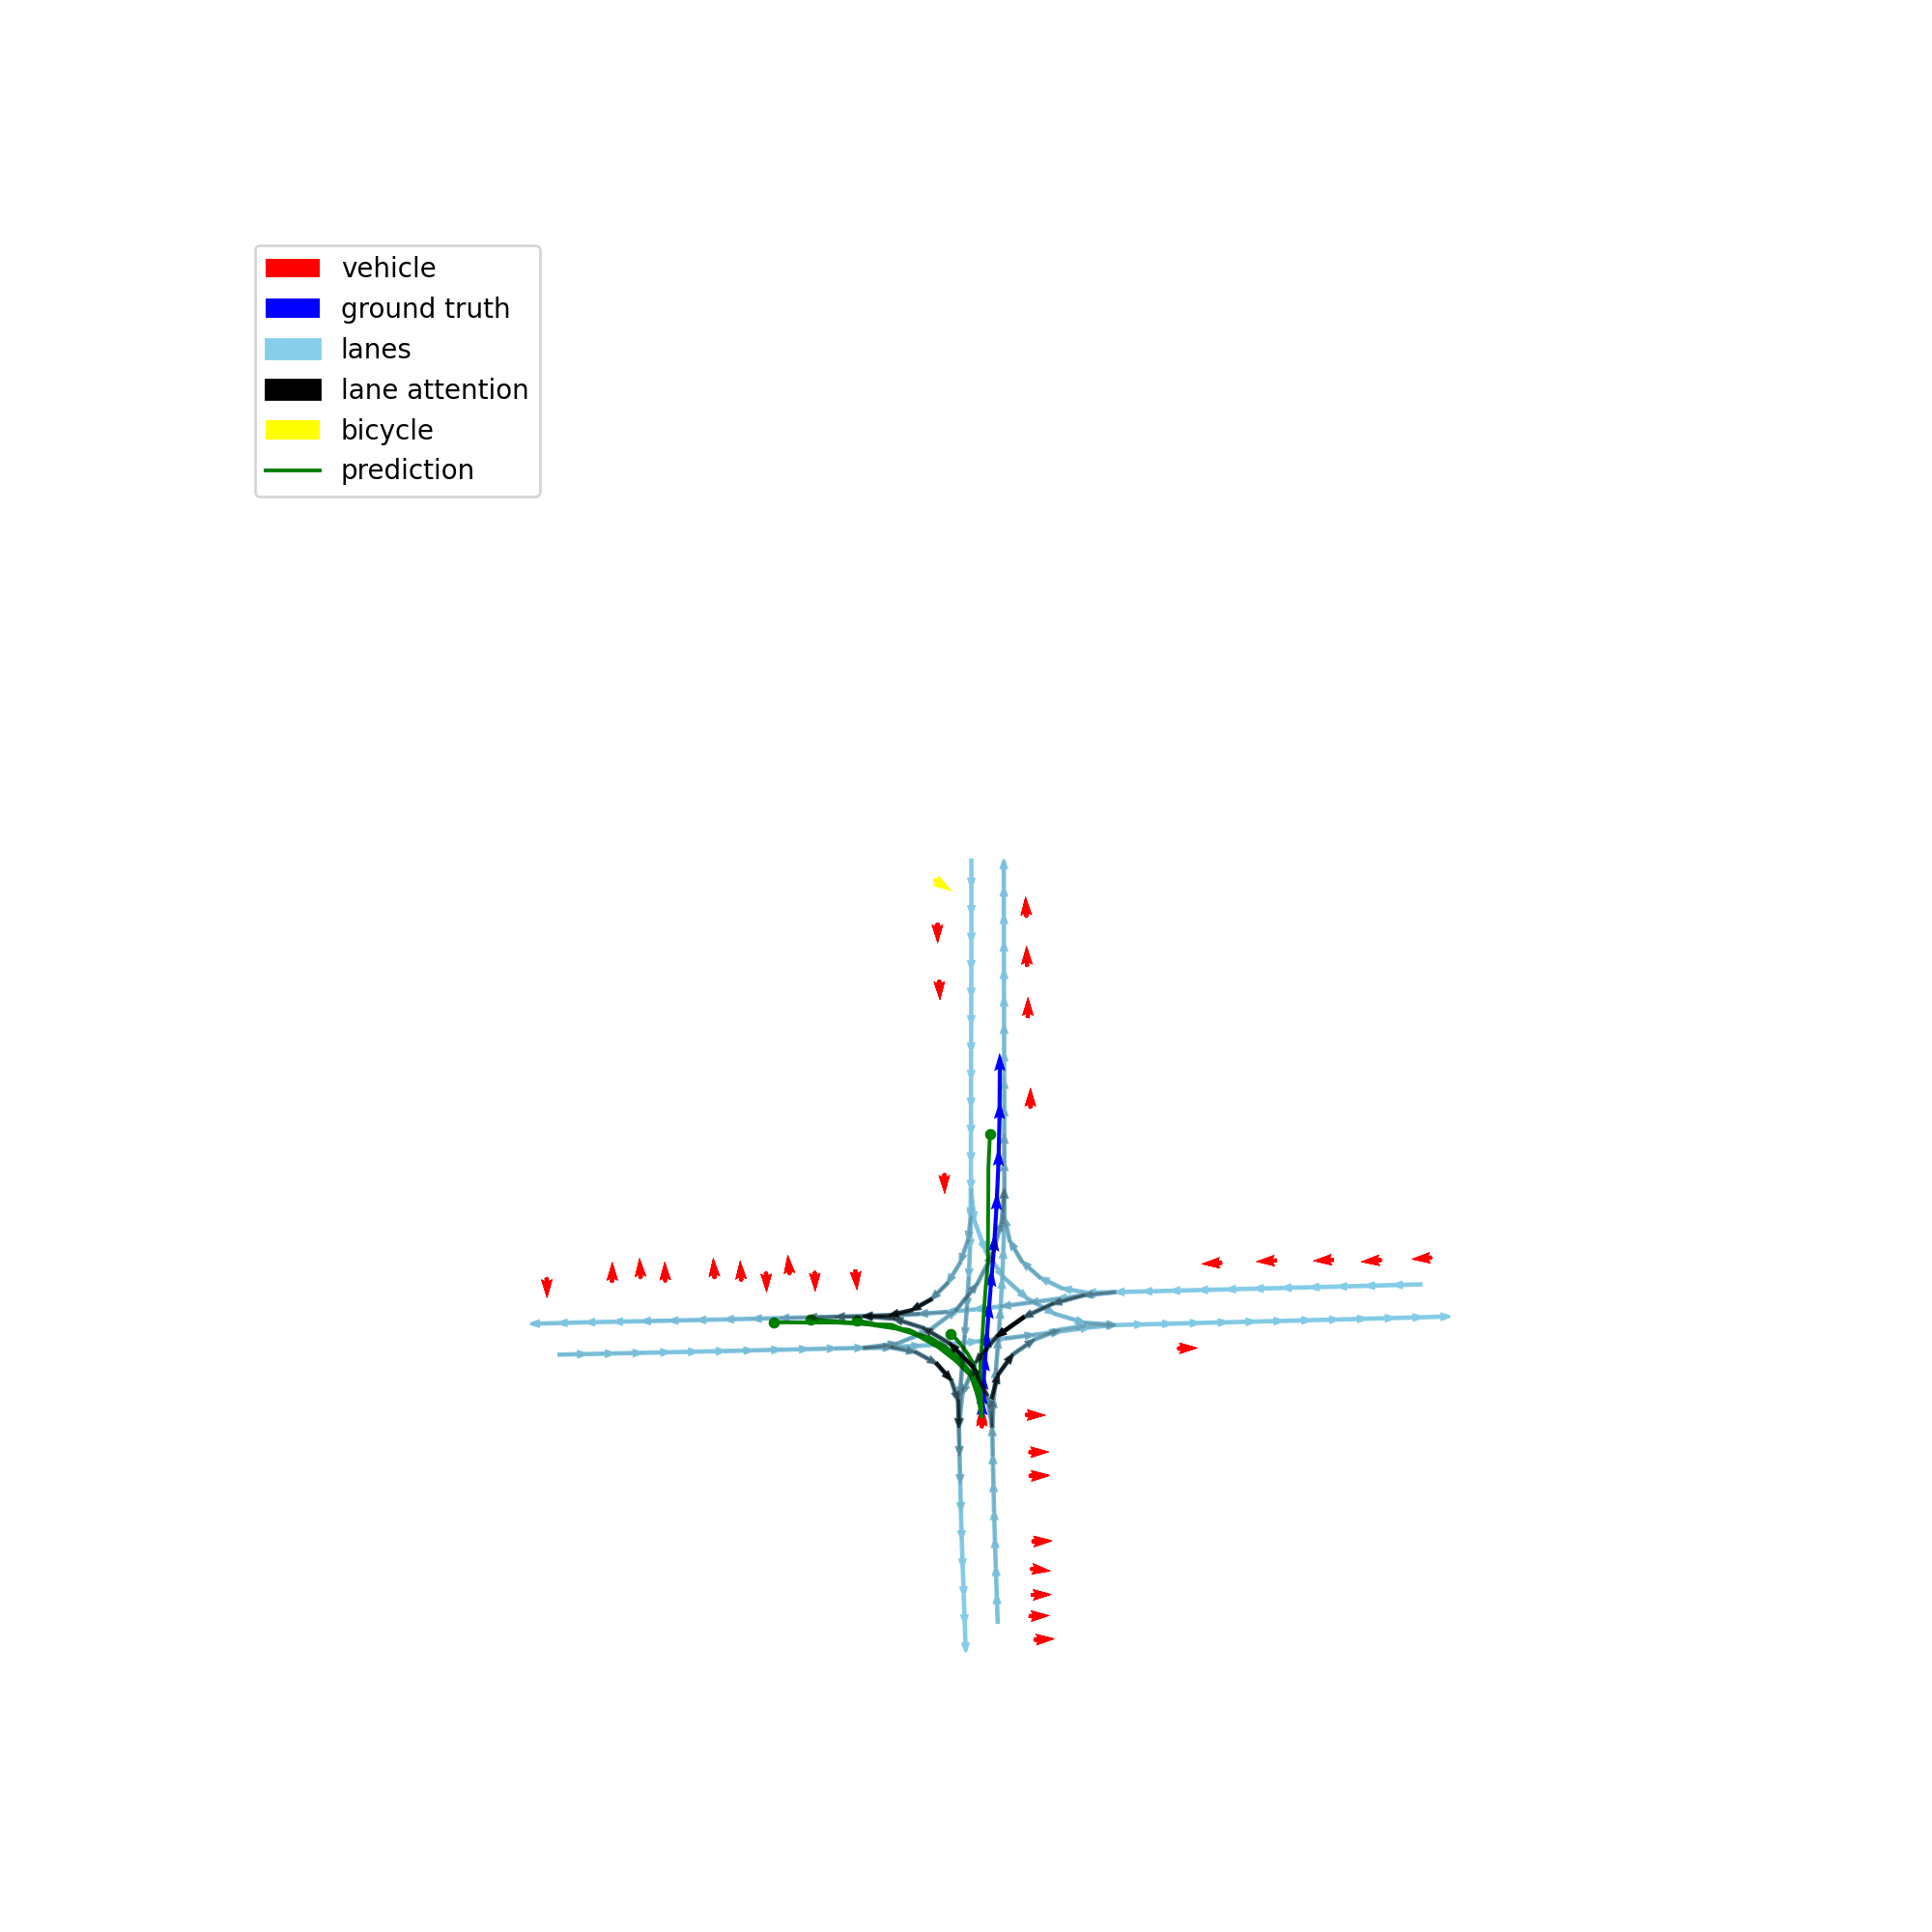
\includegraphics[height=3cm,trim={280 170 300 380},clip]{images_results/1337_minADE5_9.3_2-min.png}
        \caption{Final}
    \end{subfigure}
    % \begin{tikzpicture}[remember picture,overlay]
    %  \node at (0,3)      {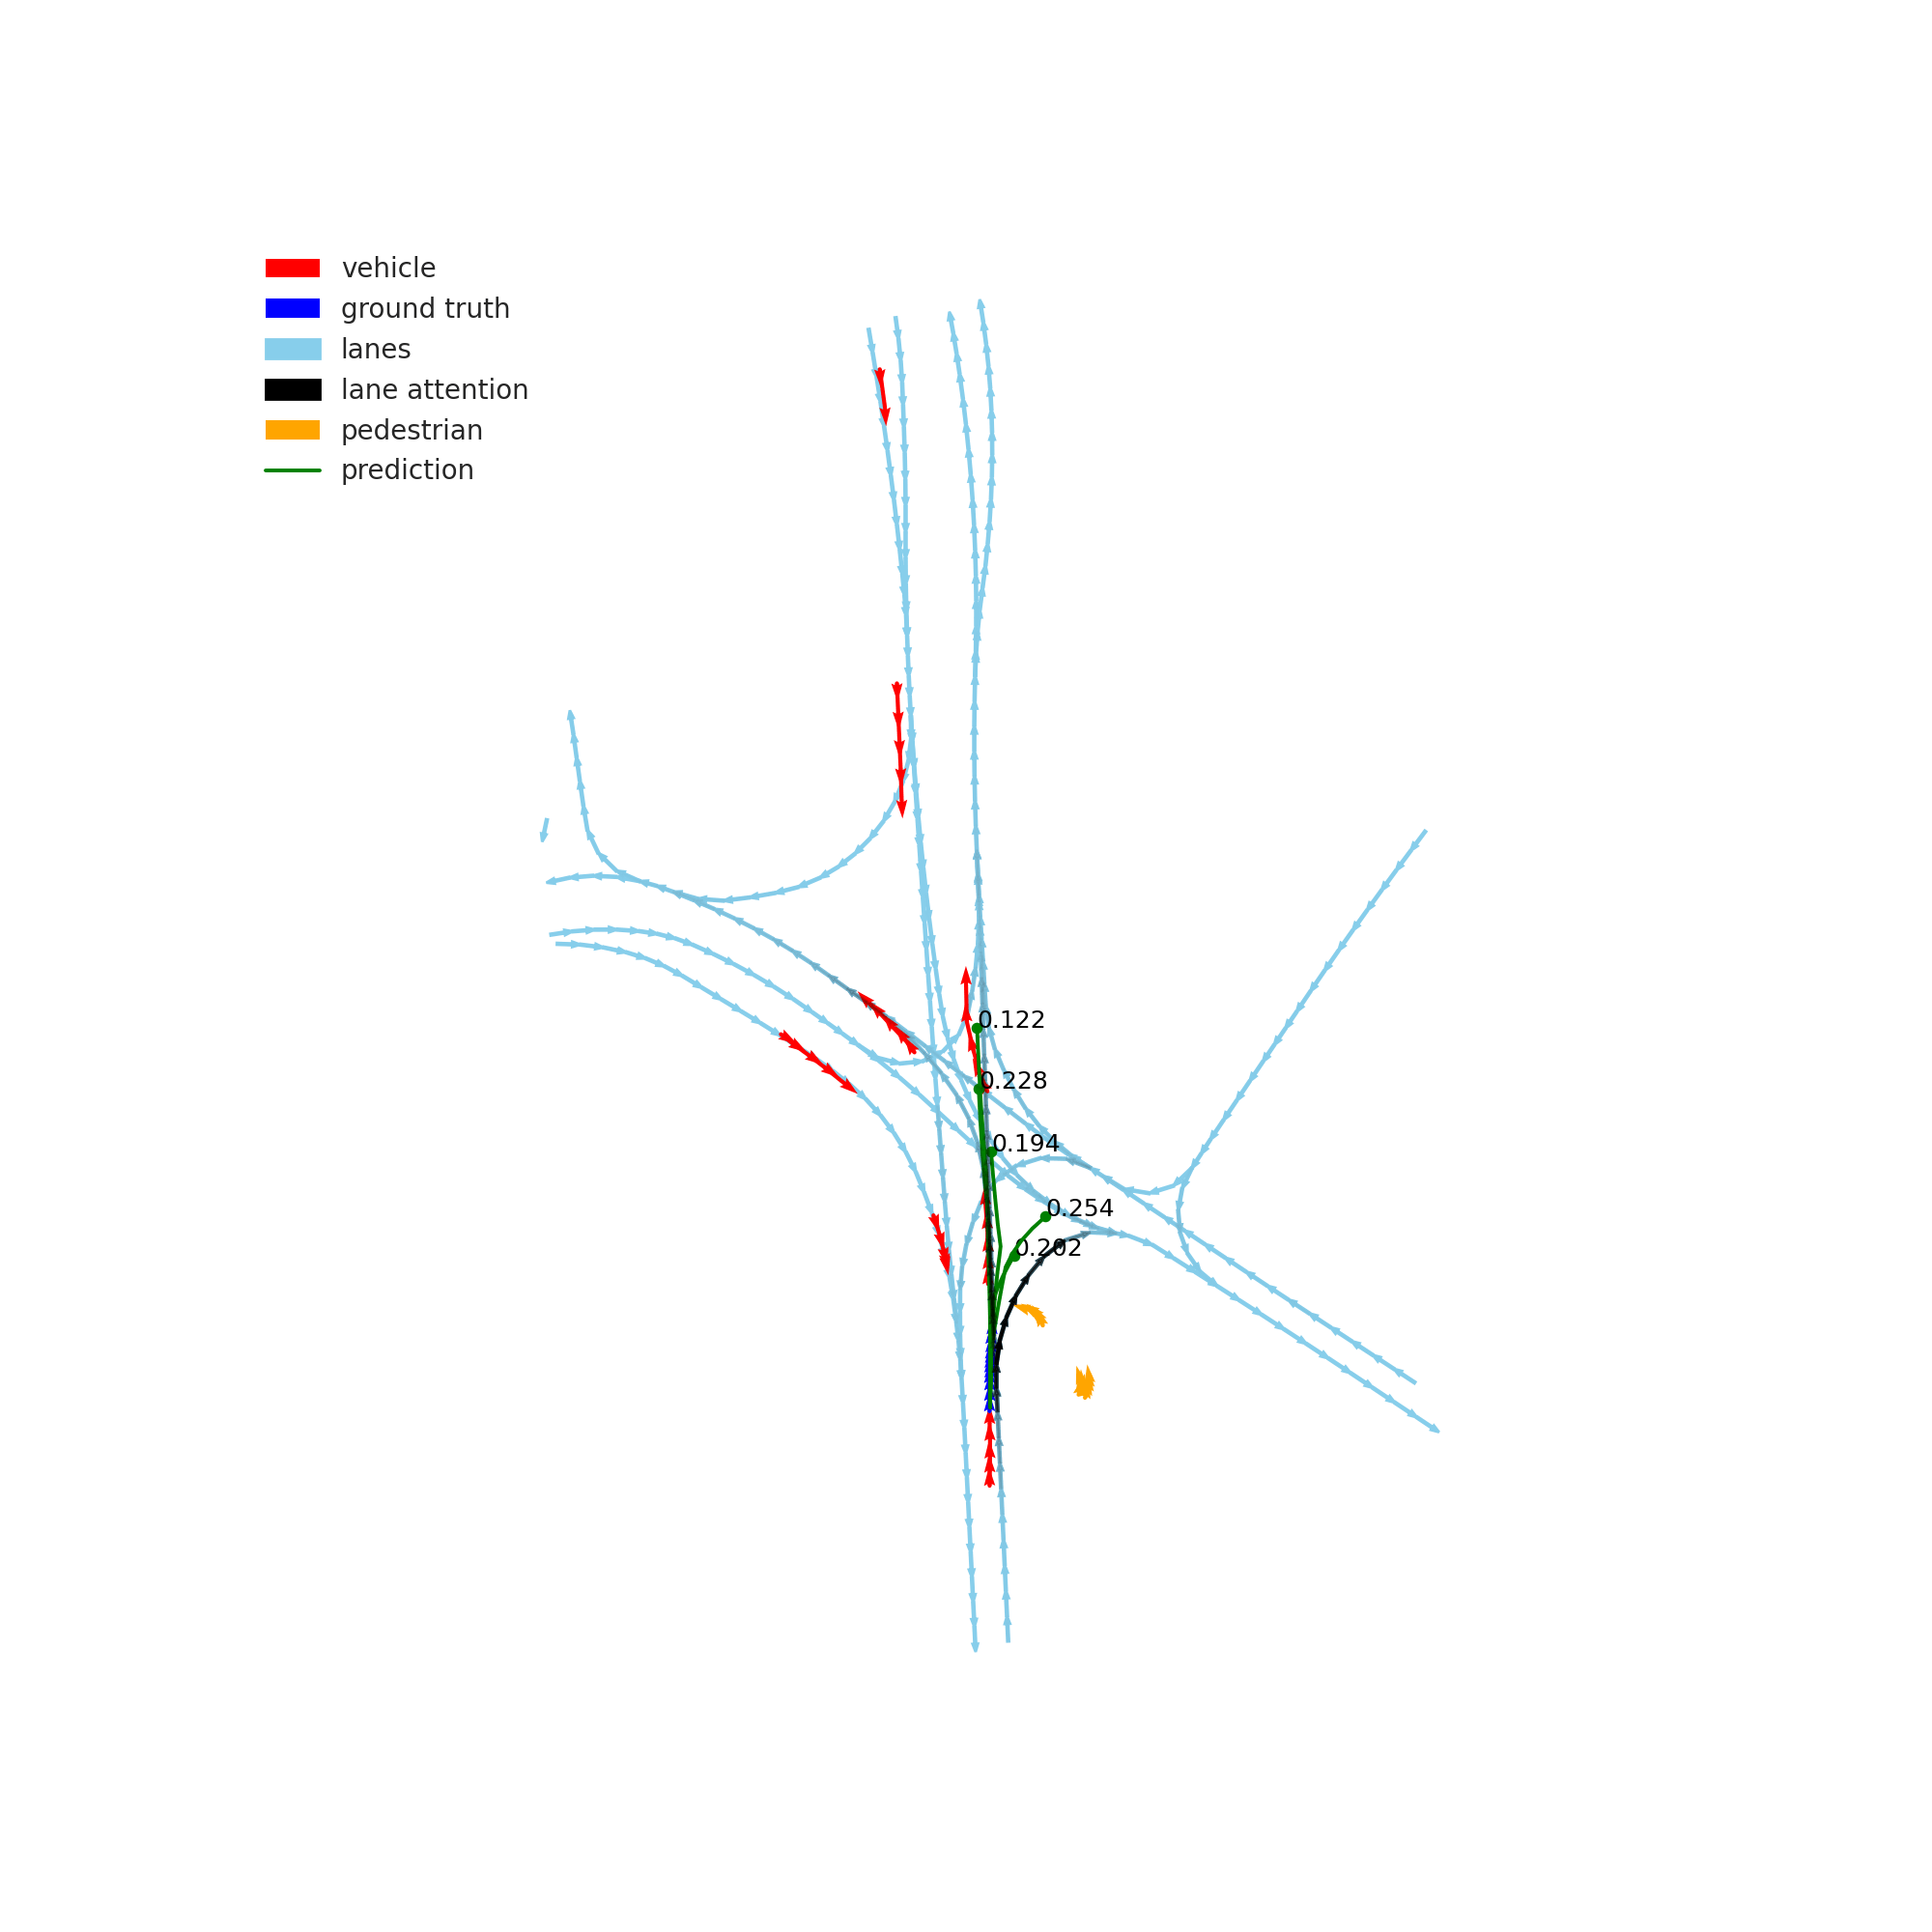
\includegraphics[width=0.2\linewidth,trim={110 500 450 85},clip]{images_results/2706cc4eb61844a1a5c7a5cb766ffc2e_37ab2d88d07846ef96d5227e9c5a15d7_minADE5_5.01_0-min.png}};
    % \end{tikzpicture}
    \caption{Visualization of predicted trajectories (green) for a target agent at an unseen intersection during training. The model, trained on the Deep Scenario dataset, refines its predictions progressively from (a) to (c), achieving better alignment with the lane structure. However, as shown in the second row, a limitation of our approach becomes evident: despite the attention maps indicating that the network should predict right-turn trajectories, it fails to generate them.}
    \label{fig:cross_data_qual}    
\end{figure}

\begin{table}[b]
    \centering
    \caption{LMFormer Cross Datataset performance validated on nuScenes validation split}
    \label{tab:train_ds_eval_nuScenes}
    \resizebox{\linewidth}{!}{
    \begin{tabular}{c c|c c c|c}
    \hline
    \multicolumn{2}{c|}{Training Dataset} & & & & \\
    Deep Scenario & nuScenes & minADE\textsubscript{5}$\downarrow$ & MR\textsubscript{5}$\downarrow$ & minFDE\textsubscript{5}$\downarrow$ & OffRoad$\downarrow$ \\
    \hline
    \checkmark & - & 1.54 & 0.57 & 2.86 & 0.02\\
    - & \checkmark & 1.13 & 0.48 & 2.13 & 0.01 \\
    \checkmark &\checkmark & 1.10 & 0.46 & 2.07 & 0.01\\
    \hline
    % \checkmark & - & 1.56 & 0.57 & 3.02 & 0.02 \\
    % - & \checkmark & 1.13 & 0.47 & 2.14 & 0.01 \\
    % \checkmark &\checkmark & 1.10 & 0.44 & 2.09 & 0.01\\
    \end{tabular}
    }
\end{table}

Furthermore, a quantitative evaluation of this model checkpoint, which is trained on Deep Scenario, is done on the nuScenes validation split to assess its cross-dataset generalization capabilities. The corresponding results are presented in Table \ref{tab:train_ds_eval_nuScenes}. It can be observed that the performance of this model checkpoint is significantly worse in comparison to the one trained on the nuScenes training set. In our analysis of this cross-dataset performance degradation, we identified a systematic underestimation of the predicted velocity in the case of Deep Scenario as compared to nuScenes. We attribute this discrepancy to the distributional differences between the datasets: Deep Scenario captures mainly slow-moving vehicles in intersection-heavy environments, while nuScenes provides a more diverse range of driving dynamics. To test this hypothesis, we train LMFormer on a combined dataset, containing training samples from both the nuScenes and Deep Scenario training sets. The corresponding qualitative results are shown in Table \ref{tab:train_ds_eval_nuScenes}. We observe that this model checkpoint outperforms the others trained individually on Deep Scenario and nuScenes training sets. This indicates that the network can learn to generalize better with more diverse datasets and can overcome limitations present in individual datasets, as previously reported in UniTraj \cite{feng2024unitraj}. It is important to note that the network architecture as well as the number of parameters were kept constant in the cross-dataset evaluations. 

In addition, we also illustrate the capability of LMFormer to predict multiple agents in parallel. Figure \ref{fig:scene_prediction} shows a marginal scene prediction output, where the trajectories are predicted in a single forward pass for all vehicles in the scene. 
\begin{figure}
    \centering
    \begin{subfigure}[t]{0.4\linewidth}
        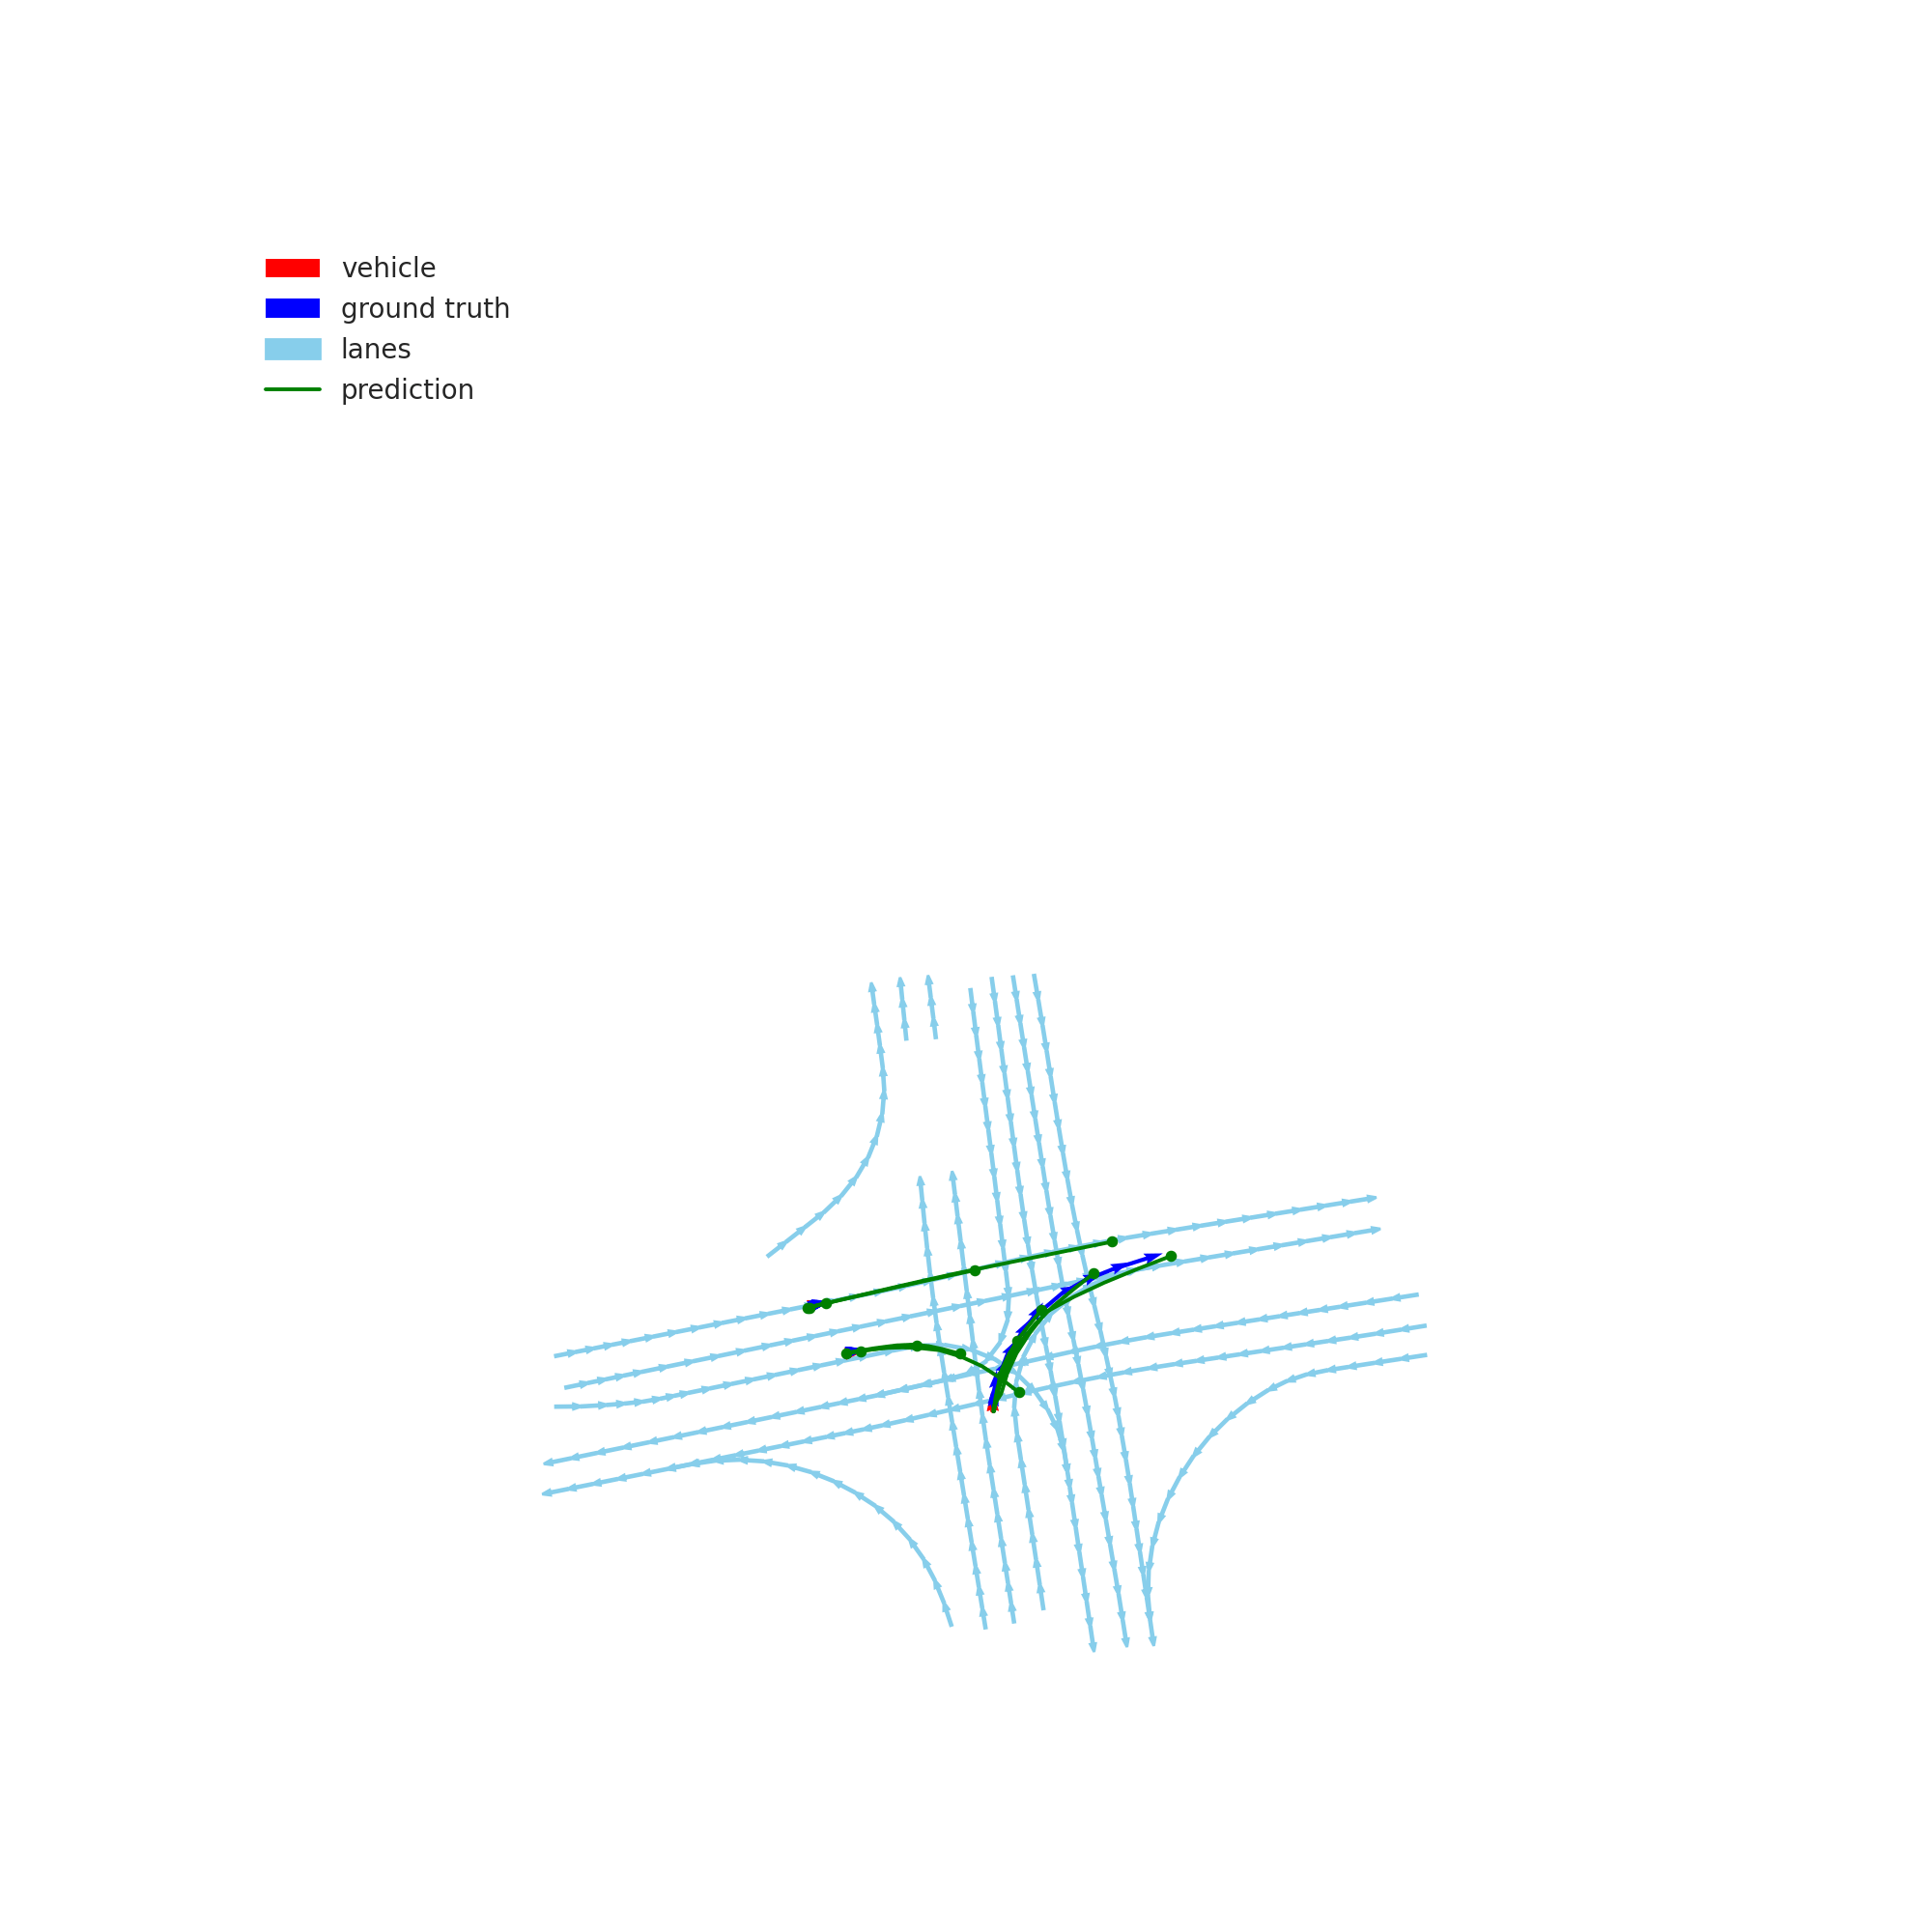
\includegraphics[height=4cm,trim={270 100 250 350},clip]{images_results/0044aaa230fe4cbeb4b744031e33af29_fb907b8b05644df28d64d6e25e9a956c_2-min.png}
        % \caption{Final Trajectories}
    \end{subfigure}
    \begin{subfigure}[t]{0.2\linewidth}
        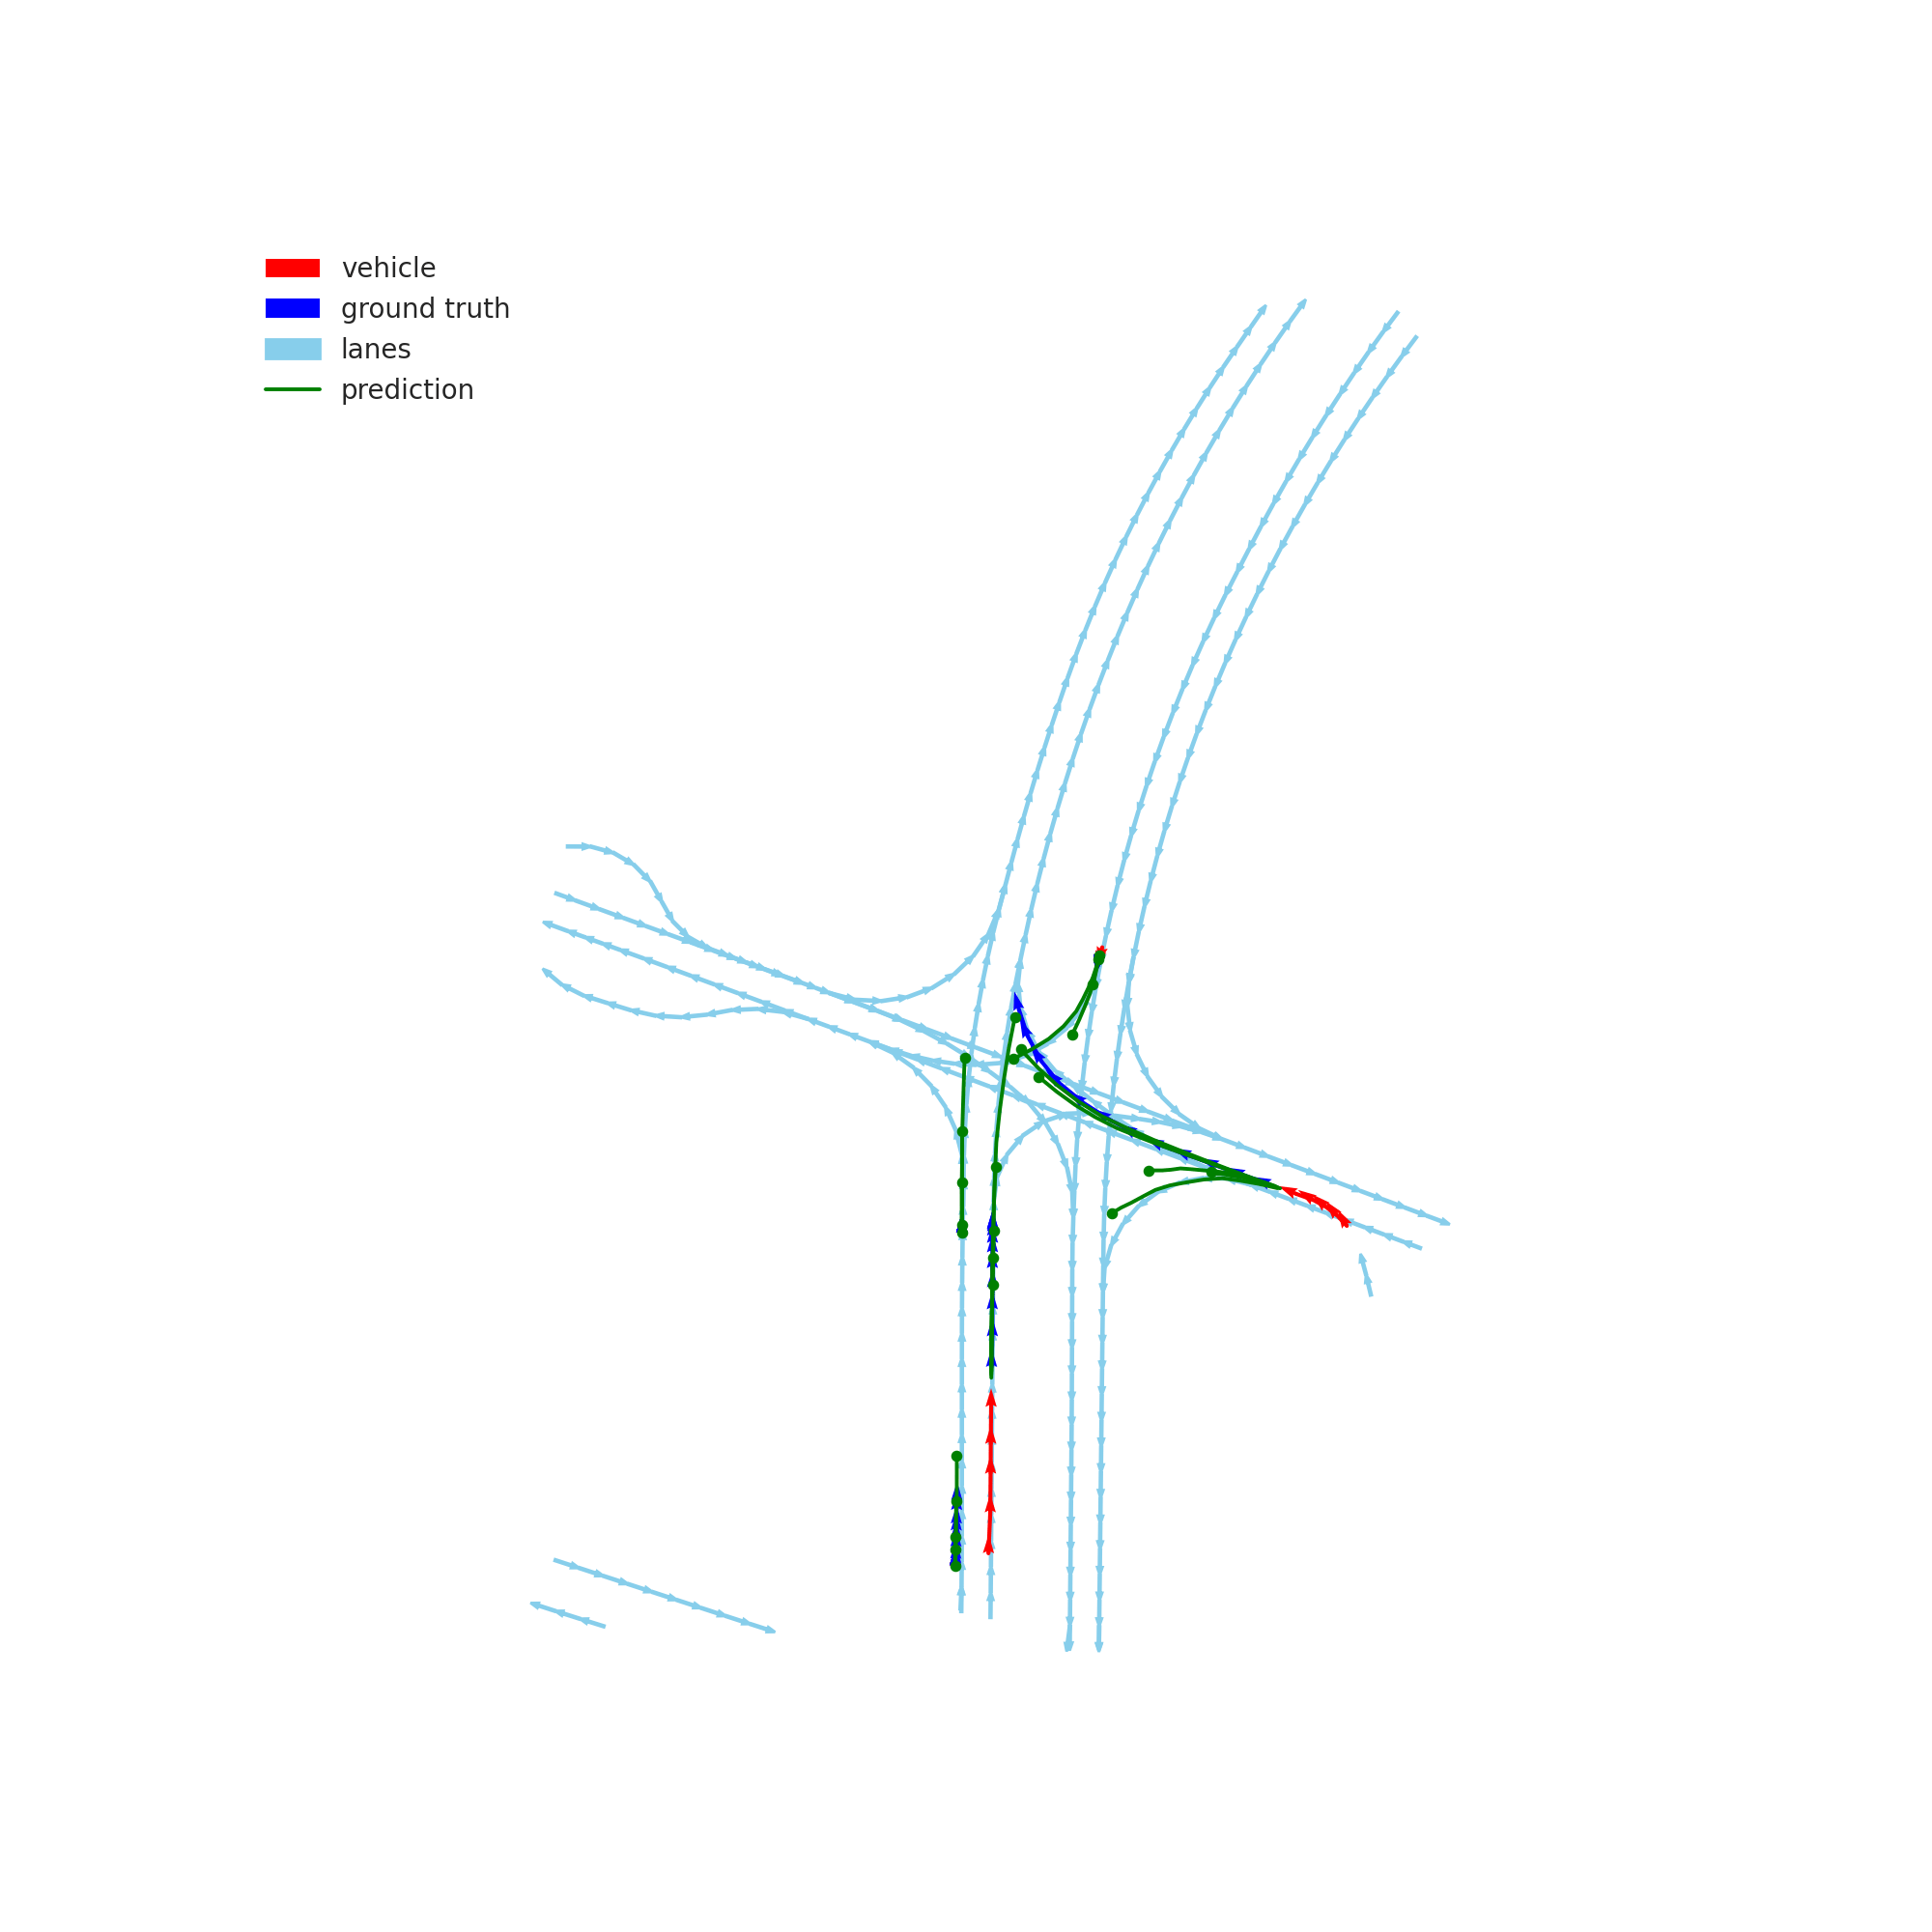
\includegraphics[height=4cm,trim={280 130 240 300},clip]{images_results/6c245e7d868c4be5a9c23c816701b103_c03d17123c6345f1a4626c6245b2c962_2-min.png}
        % \caption{Final Trajectories}
    \end{subfigure}
    % \begin{tikzpicture}[remember picture,overlay]
    %  \node at (0,7)      {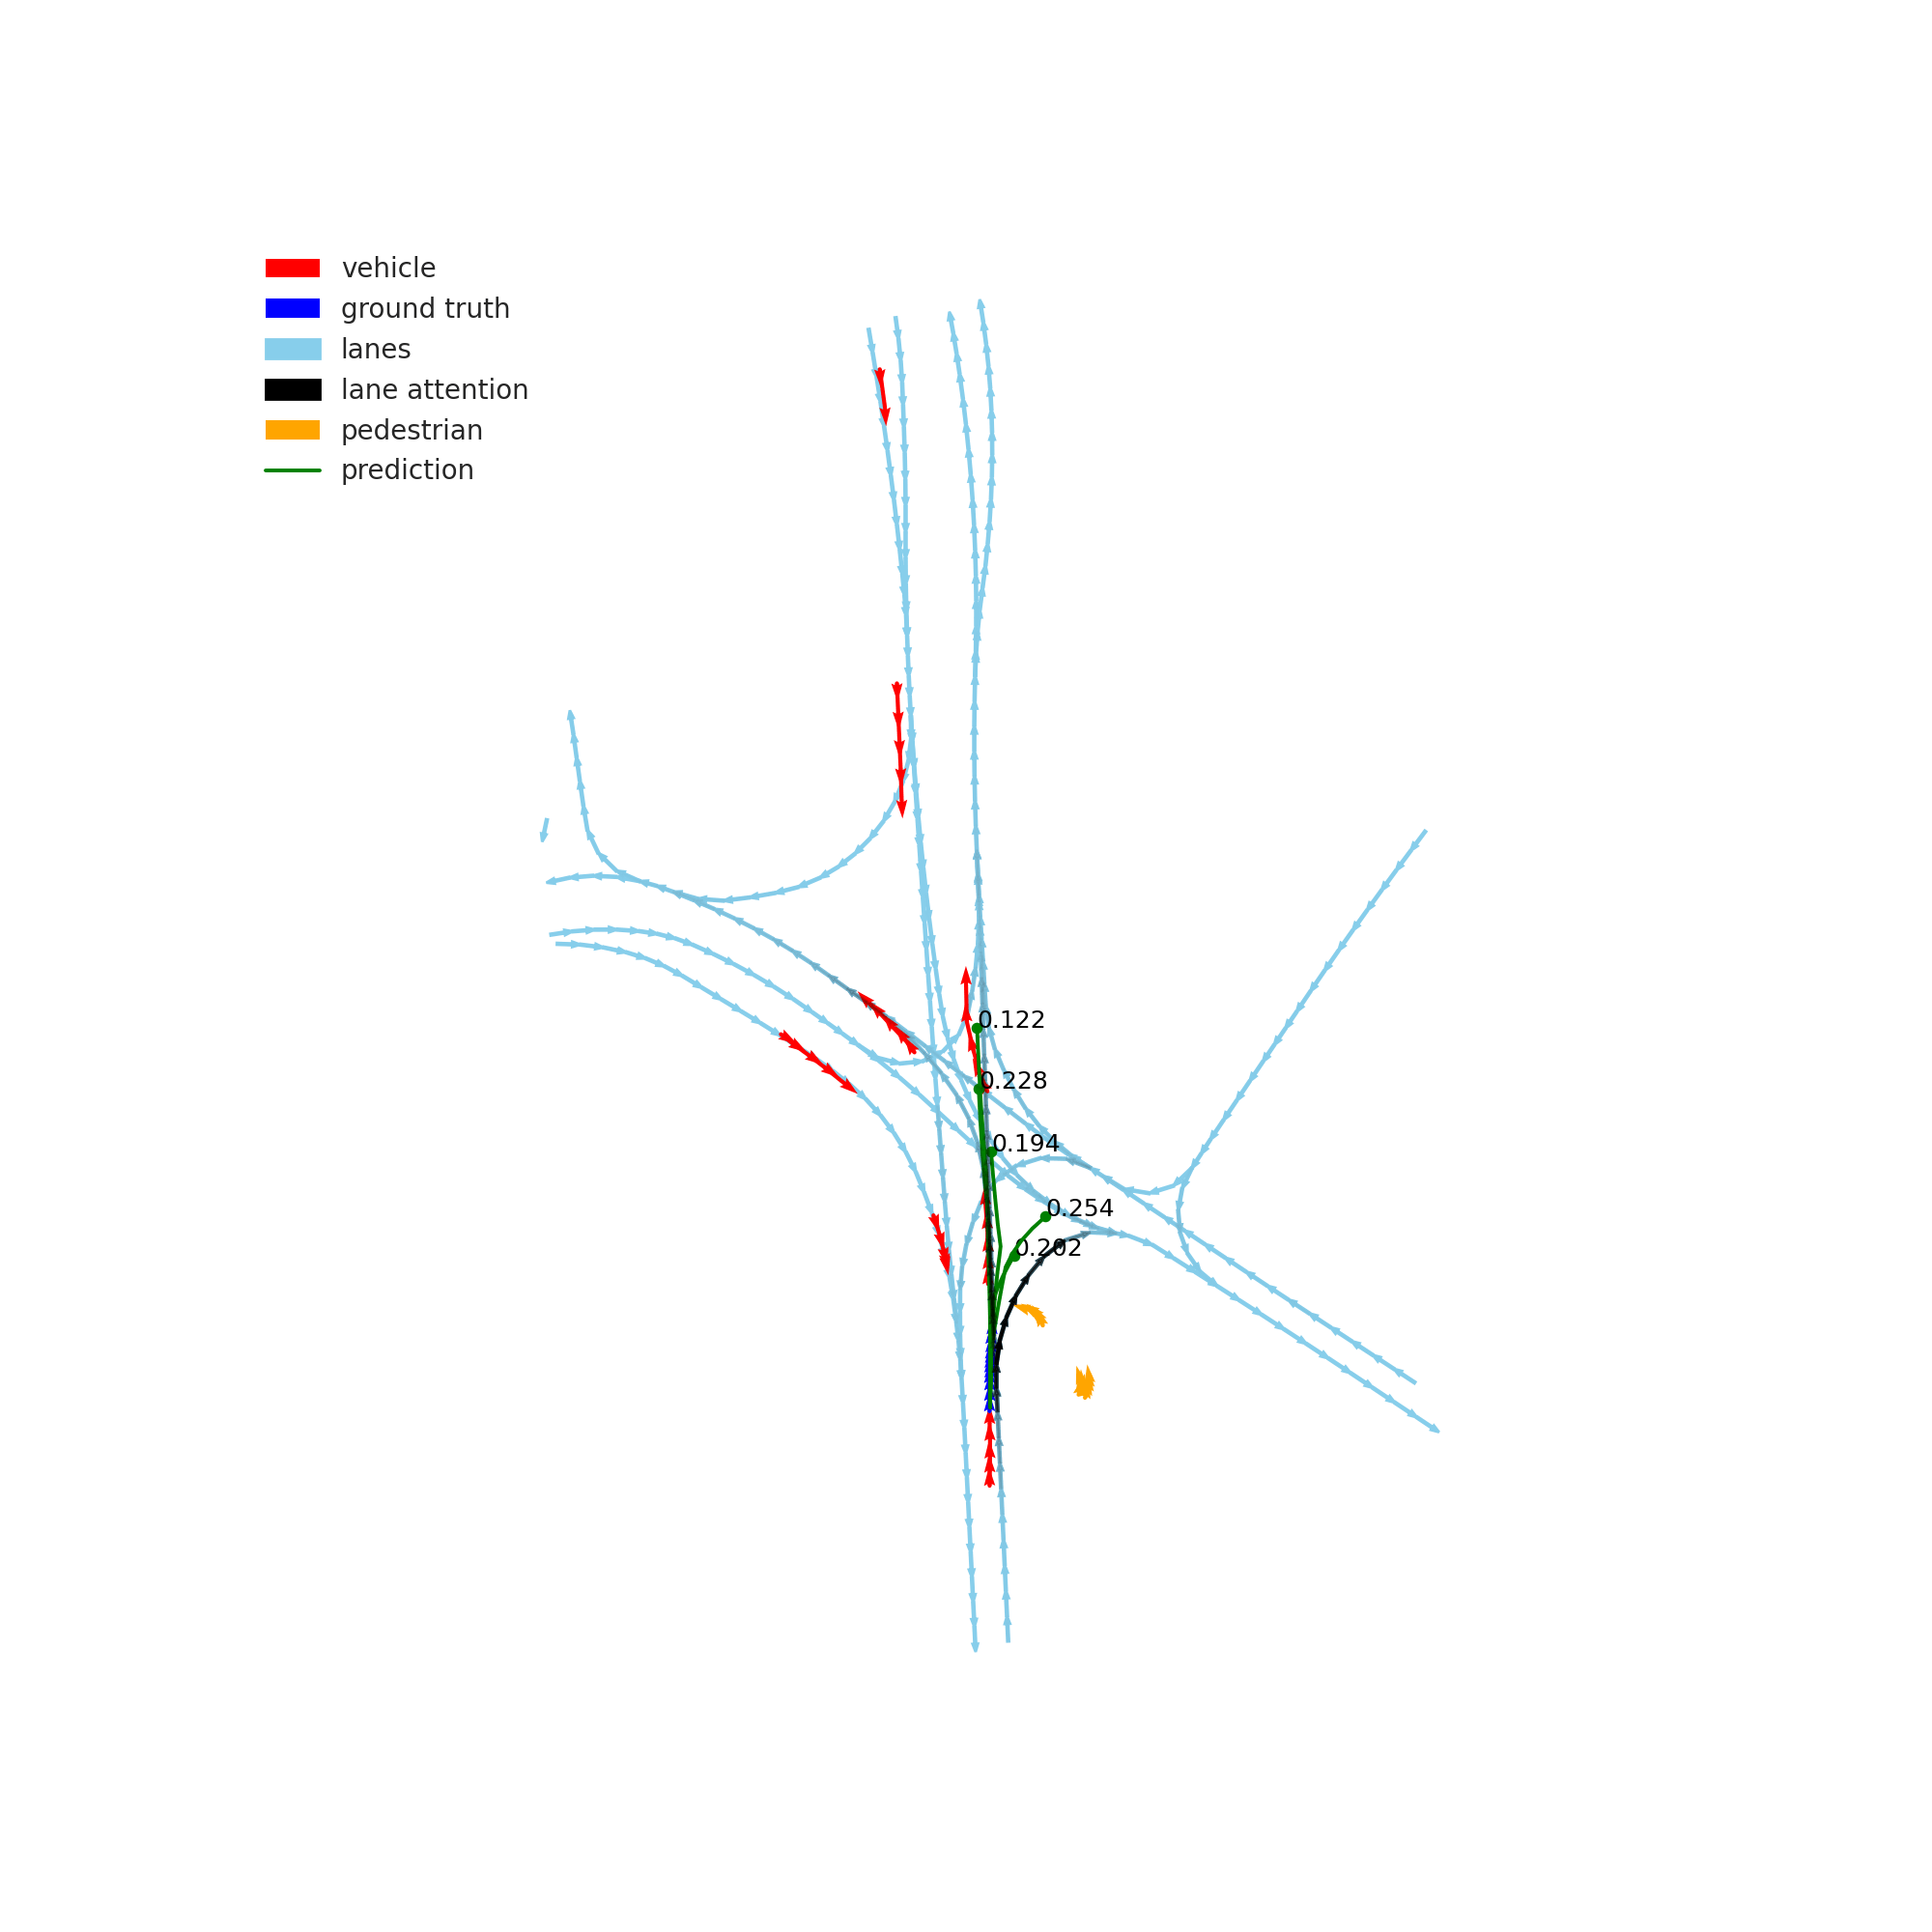
\includegraphics[width=0.2\linewidth,trim={110 500 450 30},clip]{images_results/2706cc4eb61844a1a5c7a5cb766ffc2e_37ab2d88d07846ef96d5227e9c5a15d7_minADE5_5.01_0-min.png}};
    % \end{tikzpicture}
    \caption{A depiction of marginal scene prediction. It illustrates the capability that LMFormer can be extended to multi-agent prediction.}
    \label{fig:scene_prediction}    
\end{figure}


\subsection{Ablations}\label{subsection:ablations}
In our ablation study, we validate the two key components of our approach: (1) the refinement strategy and (2) the long-range lane encoder. To evaluate the impact of refinement, we remove the additional regression loss introduced by the refinement layers. Similarly, we remove the lane self-attention module to evaluate the role of long-range lane interactions within the Map Encoder. The results of the ablation are presented in Table \ref{tab:ablation}. These results show that removing either component leads to a degradation in performance, with the degradation being slightly more pronounced when refinement losses are omitted. Overall, the ablation study confirms that both proposed components contribute significantly to SOTA performance.

\begin{table}[h]
    \centering
    \caption{Ablation Study conducted on the nuScenes val split}
    \label{tab:ablation}
    \resizebox{\linewidth}{!}{
    \begin{tabular}{c c|c c c|c}
    \hline
    \makecell{Lane \\ Self Attention} & Refinement & minADE\textsubscript{5}$\downarrow$ & MR\textsubscript{5}$\downarrow$ & minFDE\textsubscript{5}$\downarrow$ & OffRoad$\downarrow$ \\
    \hline
    \checkmark & \checkmark & 1.13 & 0.48 & 2.13 & 0.01 \\
     \checkmark & - & 1.16 & 0.51 & 2.20 & 0.01 \\
    - & \checkmark & 1.15 & 0.49 & 2.19 & 0.01 \\
    \hline
    %  \checkmark & \checkmark & 1.13 & 0.47 & 2.14 & 0.01 \\
    %  \checkmark & - & 1.14 & 0.48 & 2.16 & 0.01 \\
    %  \checkmark & - & 1.15 & 0.48 & 2.16 & 0.01 \\
    % - & \checkmark & 1.15 & 0.47 & 2.19 & 0.01 \\
    % - & \checkmark & 1.15 & 0.47 & 2.18 & 0.01 \\
    \end{tabular}
    }
\end{table}
\section{Conclusion}
The paper introduces a transformer-based motion prediction module and tackles several important challenges such as trajectory refinement and lane attention. Our work establishes that lanes are the most important components in the static context for prediction tasks. Although LMFormer quantitatively achieves SOTA performance, the qualitative results show that further improvements are needed to address robustness in prediction diversity. We also note that the current evaluation benchmarks are limited in scope and could benefit from additional metrics for velocity profiles and predicted paths. Our cross-dataset evaluation highlights a potential limitation of training on intersection-centric data when generalizing to broader urban driving scenarios, but this issue could be overcome by combining samples from individual datasets.
{
    \small
    \bibliographystyle{ieeenat_fullname}
    \bibliography{main}
}

% WARNING: do not forget to delete the supplementary pages from your submission 
% \clearpage
\setcounter{page}{1}
\maketitlesupplementary


\section{Rationale}
\label{sec:rationale}
% 
Having the supplementary compiled together with the main paper means that:
% 
\begin{itemize}
\item The supplementary can back-reference sections of the main paper, for example, we can refer to \cref{sec:intro};
\item The main paper can forward reference sub-sections within the supplementary explicitly (e.g. referring to a particular experiment); 
\item When submitted to arXiv, the supplementary will already included at the end of the paper.
\end{itemize}
% 
To split the supplementary pages from the main paper, you can use \href{https://support.apple.com/en-ca/guide/preview/prvw11793/mac#:~:text=Delete%20a%20page%20from%20a,or%20choose%20Edit%20%3E%20Delete).}{Preview (on macOS)}, \href{https://www.adobe.com/acrobat/how-to/delete-pages-from-pdf.html#:~:text=Choose%20%E2%80%9CTools%E2%80%9D%20%3E%20%E2%80%9COrganize,or%20pages%20from%20the%20file.}{Adobe Acrobat} (on all OSs), as well as \href{https://superuser.com/questions/517986/is-it-possible-to-delete-some-pages-of-a-pdf-document}{command line tools}.

\end{document}
